\documentclass[twoside]{book}

% Packages required by doxygen
\usepackage{calc}
\usepackage{doxygen}
\usepackage{graphicx}
\usepackage[utf8]{inputenc}
\usepackage{makeidx}
\usepackage{multicol}
\usepackage{multirow}
\usepackage{textcomp}
\usepackage[table]{xcolor}

% Font selection
\usepackage[T1]{fontenc}
\usepackage{mathptmx}
\usepackage[scaled=.90]{helvet}
\usepackage{courier}
\usepackage{amssymb}
\usepackage{sectsty}
\renewcommand{\familydefault}{\sfdefault}
\allsectionsfont{%
  \fontseries{bc}\selectfont%
  \color{darkgray}%
}
\renewcommand{\DoxyLabelFont}{%
  \fontseries{bc}\selectfont%
  \color{darkgray}%
}

% Page & text layout
\usepackage{geometry}
\geometry{%
  a4paper,%
  top=2.5cm,%
  bottom=2.5cm,%
  left=2.5cm,%
  right=2.5cm%
}
\tolerance=750
\hfuzz=15pt
\hbadness=750
\setlength{\emergencystretch}{15pt}
\setlength{\parindent}{0cm}
\setlength{\parskip}{0.2cm}
\makeatletter
\renewcommand{\paragraph}{%
  \@startsection{paragraph}{4}{0ex}{-1.0ex}{1.0ex}{%
    \normalfont\normalsize\bfseries\SS@parafont%
  }%
}
\renewcommand{\subparagraph}{%
  \@startsection{subparagraph}{5}{0ex}{-1.0ex}{1.0ex}{%
    \normalfont\normalsize\bfseries\SS@subparafont%
  }%
}
\makeatother

% Headers & footers
\usepackage{fancyhdr}
\pagestyle{fancyplain}
\fancyhead[LE]{\fancyplain{}{\bfseries\thepage}}
\fancyhead[CE]{\fancyplain{}{}}
\fancyhead[RE]{\fancyplain{}{\bfseries\leftmark}}
\fancyhead[LO]{\fancyplain{}{\bfseries\rightmark}}
\fancyhead[CO]{\fancyplain{}{}}
\fancyhead[RO]{\fancyplain{}{\bfseries\thepage}}
\fancyfoot[LE]{\fancyplain{}{}}
\fancyfoot[CE]{\fancyplain{}{}}
\fancyfoot[RE]{\fancyplain{}{\bfseries\scriptsize Generated on Mon Jun 19 2023 13\-:45\-:07 for Lib\-Man -\/ Open Source Library Manager Documentation by Doxygen }}
\fancyfoot[LO]{\fancyplain{}{\bfseries\scriptsize Generated on Mon Jun 19 2023 13\-:45\-:07 for Lib\-Man -\/ Open Source Library Manager Documentation by Doxygen }}
\fancyfoot[CO]{\fancyplain{}{}}
\fancyfoot[RO]{\fancyplain{}{}}
\renewcommand{\footrulewidth}{0.4pt}
\renewcommand{\chaptermark}[1]{%
  \markboth{#1}{}%
}
\renewcommand{\sectionmark}[1]{%
  \markright{\thesection\ #1}%
}

% Indices & bibliography
\usepackage{natbib}
\usepackage[titles]{tocloft}
\setcounter{tocdepth}{3}
\setcounter{secnumdepth}{5}
\makeindex

% Hyperlinks (required, but should be loaded last)
\usepackage{ifpdf}
\ifpdf
  \usepackage[pdftex,pagebackref=true]{hyperref}
\else
  \usepackage[ps2pdf,pagebackref=true]{hyperref}
\fi
\hypersetup{%
  colorlinks=true,%
  linkcolor=blue,%
  citecolor=blue,%
  unicode%
}

% Custom commands
\newcommand{\clearemptydoublepage}{%
  \newpage{\pagestyle{empty}\cleardoublepage}%
}


%===== C O N T E N T S =====

\begin{document}

% Titlepage & ToC
\hypersetup{pageanchor=false}
\pagenumbering{roman}
\begin{titlepage}
\vspace*{7cm}
\begin{center}%
{\Large Lib\-Man -\/ Open Source Library Manager Documentation \\[1ex]\large 1.\-0 }\\
\vspace*{1cm}
{\large Generated by Doxygen 1.8.5}\\
\vspace*{0.5cm}
{\small Mon Jun 19 2023 13:45:07}\\
\end{center}
\end{titlepage}
\clearemptydoublepage
\tableofcontents
\clearemptydoublepage
\pagenumbering{arabic}
\hypersetup{pageanchor=true}

%--- Begin generated contents ---
\chapter{Copyright 2023 I\-H\-P Lib\-Man Authors}
\label{index}\hypertarget{index}{}



Licensed under the Apache License, Version 2.\-0 (the "License") you may not use this file except in compliance with the License You may obtain a copy of the License at \href{https://www.apache.org/licenses/LICENSE-2.0}{\tt https\-://www.\-apache.\-org/licenses/\-L\-I\-C\-E\-N\-S\-E-\/2.\-0} Unless required by applicable law or agreed to in writing, software distributed under the License is distributed on an "A\-S I\-S" B\-A\-S\-I\-S, W\-I\-T\-H\-O\-U\-T W\-A\-R\-R\-A\-N\-T\-I\-E\-S O\-R C\-O\-N\-D\-I\-T\-I\-O\-N\-S O\-F A\-N\-Y K\-I\-N\-D, either express or implied. See the License for the specific language governing permissions and limitations under the License. 
\chapter{Hierarchical Index}
\section{Class Hierarchy}
This inheritance list is sorted roughly, but not completely, alphabetically\-:\begin{DoxyCompactList}
\item \contentsline{section}{Properties}{\pageref{classProperties}}{}
\item \contentsline{section}{Property\-Item}{\pageref{classPropertyItem}}{}
\item Q\-Dialog\begin{DoxyCompactList}
\item \contentsline{section}{About}{\pageref{classAbout}}{}
\item \contentsline{section}{New\-View}{\pageref{classNewView}}{}
\item \contentsline{section}{Project\-Manager}{\pageref{classProjectManager}}{}
\item \contentsline{section}{Tool\-Manager}{\pageref{classToolManager}}{}
\end{DoxyCompactList}
\item Q\-Main\-Window\begin{DoxyCompactList}
\item \contentsline{section}{Main\-Window}{\pageref{classMainWindow}}{}
\end{DoxyCompactList}
\end{DoxyCompactList}

\chapter{Class Index}
\section{Class List}
Here are the classes, structs, unions and interfaces with brief descriptions\-:\begin{DoxyCompactList}
\item\contentsline{section}{\hyperlink{classAbout}{About} \\*Creates and shows a dialog window with an information about Lib\-Man }{\pageref{classAbout}}{}
\item\contentsline{section}{\hyperlink{classMainWindow}{Main\-Window} \\*Responsible for creating main framework of Lib\-Man and controlls all slots and signals }{\pageref{classMainWindow}}{}
\item\contentsline{section}{\hyperlink{classNewView}{New\-View} \\*Creates a dialog box where user can select which view to be created }{\pageref{classNewView}}{}
\item\contentsline{section}{\hyperlink{classProjectManager}{Project\-Manager} \\*Creates a dialog window to allow user controlling Lib\-Man projects }{\pageref{classProjectManager}}{}
\item\contentsline{section}{\hyperlink{classProperties}{Properties} \\*Stores and manipulates all kind of data types. It is used for managing Lib\-Man settings }{\pageref{classProperties}}{}
\item\contentsline{section}{\hyperlink{classPropertyItem}{Property\-Item} \\*Creates a single object of any type used by the \hyperlink{classProperties}{Properties} class }{\pageref{classPropertyItem}}{}
\item\contentsline{section}{\hyperlink{classToolManager}{Tool\-Manager} \\*Creates a dialog window to allow user controlling 3-\/d party tools executed by Lib\-Man }{\pageref{classToolManager}}{}
\end{DoxyCompactList}

\chapter{Class Documentation}
\hypertarget{classAbout}{\section{About Class Reference}
\label{classAbout}\index{About@{About}}
}


The \hyperlink{classAbout}{About} class creates and shows a dialog window with an information about Lib\-Man.  




{\ttfamily \#include $<$about.\-h$>$}

Inheritance diagram for About\-:\begin{figure}[H]
\begin{center}
\leavevmode
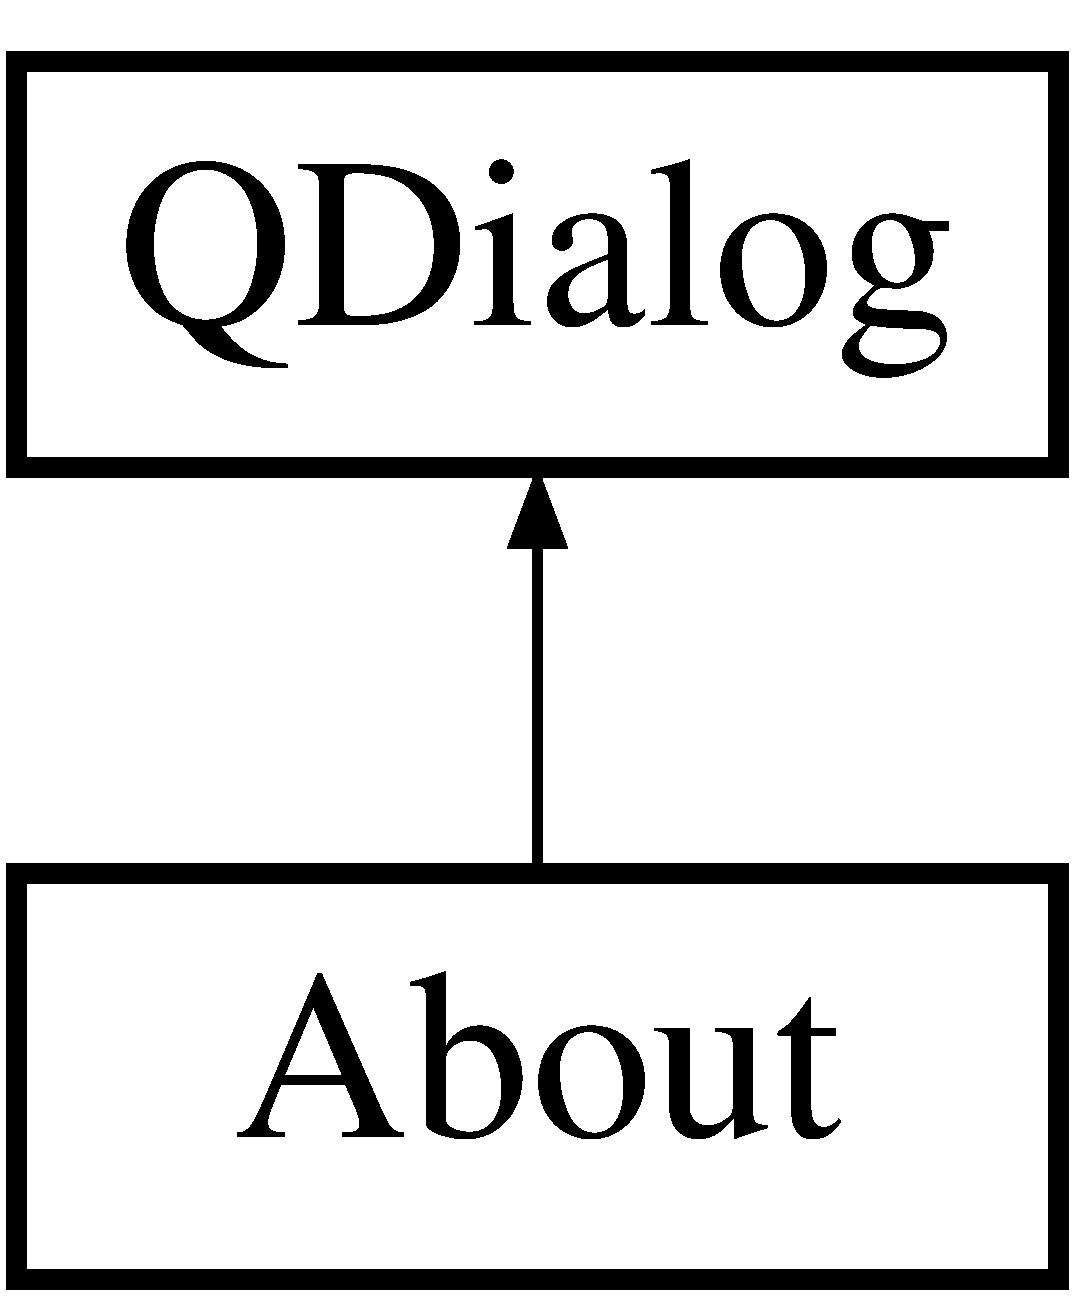
\includegraphics[height=2.000000cm]{classAbout}
\end{center}
\end{figure}
\subsection*{Public Member Functions}
\begin{DoxyCompactItemize}
\item 
\hyperlink{classAbout_ab79599ebbcdeffe0a96e00f010e64177}{About} (Q\-Widget $\ast$parent=0)
\begin{DoxyCompactList}\small\item\em Constracts \hyperlink{classAbout}{About} dialog window to show information about Lib\-Man version and its license. \end{DoxyCompactList}\item 
\hyperlink{classAbout_ace60197b1b610998908036ee1f802204}{$\sim$\-About} ()
\begin{DoxyCompactList}\small\item\em Destructs \hyperlink{classAbout}{About} obejct and clears up U\-I members. \end{DoxyCompactList}\end{DoxyCompactItemize}
\subsection*{Private Slots}
\begin{DoxyCompactItemize}
\item 
void \hyperlink{classAbout_aa6451b089d284c51ed3330eecf5a55db}{on\-\_\-btn\-Ok\-\_\-clicked} ()
\begin{DoxyCompactList}\small\item\em closes \hyperlink{classAbout}{About} window. \end{DoxyCompactList}\end{DoxyCompactItemize}
\subsection*{Private Member Functions}
\begin{DoxyCompactItemize}
\item 
Q\-String\-List \hyperlink{classAbout_a194bea41985f742b784745c95fca1b5c}{get\-License\-Text} () const 
\begin{DoxyCompactList}\small\item\em returns Apache License text for Lib\-Man. \end{DoxyCompactList}\end{DoxyCompactItemize}
\subsection*{Private Attributes}
\begin{DoxyCompactItemize}
\item 
Ui\-::\-About $\ast$ \hyperlink{classAbout_a2ed1b138dc203e50d03c7a27964a1775}{m\-\_\-ui}
\item 
Q\-String \hyperlink{classAbout_a878ee376be90c7196e05259f7abdeae2}{m\-\_\-version}
\end{DoxyCompactItemize}


\subsection{Detailed Description}
The \hyperlink{classAbout}{About} class creates and shows a dialog window with an information about Lib\-Man. 



 

\subsection{Constructor \& Destructor Documentation}
\hypertarget{classAbout_ab79599ebbcdeffe0a96e00f010e64177}{\index{About@{About}!About@{About}}
\index{About@{About}!About@{About}}
\subsubsection[{About}]{\setlength{\rightskip}{0pt plus 5cm}About\-::\-About (
\begin{DoxyParamCaption}
\item[{Q\-Widget $\ast$}]{parent = {\ttfamily 0}}
\end{DoxyParamCaption}
)\hspace{0.3cm}{\ttfamily [explicit]}}}\label{classAbout_ab79599ebbcdeffe0a96e00f010e64177}


Constracts \hyperlink{classAbout}{About} dialog window to show information about Lib\-Man version and its license. 



 
\begin{DoxyParams}{Parameters}
{\em parent} & Parent widget, by default is N\-U\-L\-L. \\
\hline
\end{DoxyParams}
\hypertarget{classAbout_ace60197b1b610998908036ee1f802204}{\index{About@{About}!$\sim$\-About@{$\sim$\-About}}
\index{$\sim$\-About@{$\sim$\-About}!About@{About}}
\subsubsection[{$\sim$\-About}]{\setlength{\rightskip}{0pt plus 5cm}About\-::$\sim$\-About (
\begin{DoxyParamCaption}
{}
\end{DoxyParamCaption}
)}}\label{classAbout_ace60197b1b610998908036ee1f802204}


Destructs \hyperlink{classAbout}{About} obejct and clears up U\-I members. 



 

\subsection{Member Function Documentation}
\hypertarget{classAbout_a194bea41985f742b784745c95fca1b5c}{\index{About@{About}!get\-License\-Text@{get\-License\-Text}}
\index{get\-License\-Text@{get\-License\-Text}!About@{About}}
\subsubsection[{get\-License\-Text}]{\setlength{\rightskip}{0pt plus 5cm}Q\-String\-List About\-::get\-License\-Text (
\begin{DoxyParamCaption}
{}
\end{DoxyParamCaption}
) const\hspace{0.3cm}{\ttfamily [private]}}}\label{classAbout_a194bea41985f742b784745c95fca1b5c}


returns Apache License text for Lib\-Man. 



 \hypertarget{classAbout_aa6451b089d284c51ed3330eecf5a55db}{\index{About@{About}!on\-\_\-btn\-Ok\-\_\-clicked@{on\-\_\-btn\-Ok\-\_\-clicked}}
\index{on\-\_\-btn\-Ok\-\_\-clicked@{on\-\_\-btn\-Ok\-\_\-clicked}!About@{About}}
\subsubsection[{on\-\_\-btn\-Ok\-\_\-clicked}]{\setlength{\rightskip}{0pt plus 5cm}void About\-::on\-\_\-btn\-Ok\-\_\-clicked (
\begin{DoxyParamCaption}
{}
\end{DoxyParamCaption}
)\hspace{0.3cm}{\ttfamily [private]}, {\ttfamily [slot]}}}\label{classAbout_aa6451b089d284c51ed3330eecf5a55db}


closes \hyperlink{classAbout}{About} window. 



 

\subsection{Member Data Documentation}
\hypertarget{classAbout_a2ed1b138dc203e50d03c7a27964a1775}{\index{About@{About}!m\-\_\-ui@{m\-\_\-ui}}
\index{m\-\_\-ui@{m\-\_\-ui}!About@{About}}
\subsubsection[{m\-\_\-ui}]{\setlength{\rightskip}{0pt plus 5cm}Ui\-::\-About$\ast$ About\-::m\-\_\-ui\hspace{0.3cm}{\ttfamily [private]}}}\label{classAbout_a2ed1b138dc203e50d03c7a27964a1775}
A pointer to acess \hyperlink{classAbout}{About} graphic items. \hypertarget{classAbout_a878ee376be90c7196e05259f7abdeae2}{\index{About@{About}!m\-\_\-version@{m\-\_\-version}}
\index{m\-\_\-version@{m\-\_\-version}!About@{About}}
\subsubsection[{m\-\_\-version}]{\setlength{\rightskip}{0pt plus 5cm}Q\-String About\-::m\-\_\-version\hspace{0.3cm}{\ttfamily [private]}}}\label{classAbout_a878ee376be90c7196e05259f7abdeae2}
Keeps information about Lib\-Man version. 

The documentation for this class was generated from the following files\-:\begin{DoxyCompactItemize}
\item 
about.\-h\item 
about.\-cpp\end{DoxyCompactItemize}

\hypertarget{classMainWindow}{\section{Main\-Window Class Reference}
\label{classMainWindow}\index{Main\-Window@{Main\-Window}}
}


The \hyperlink{classMainWindow}{Main\-Window} class is responsible for creating main framework of Lib\-Man and controlls all slots and signals.  




{\ttfamily \#include $<$mainwindow.\-h$>$}

Inheritance diagram for Main\-Window\-:\begin{figure}[H]
\begin{center}
\leavevmode
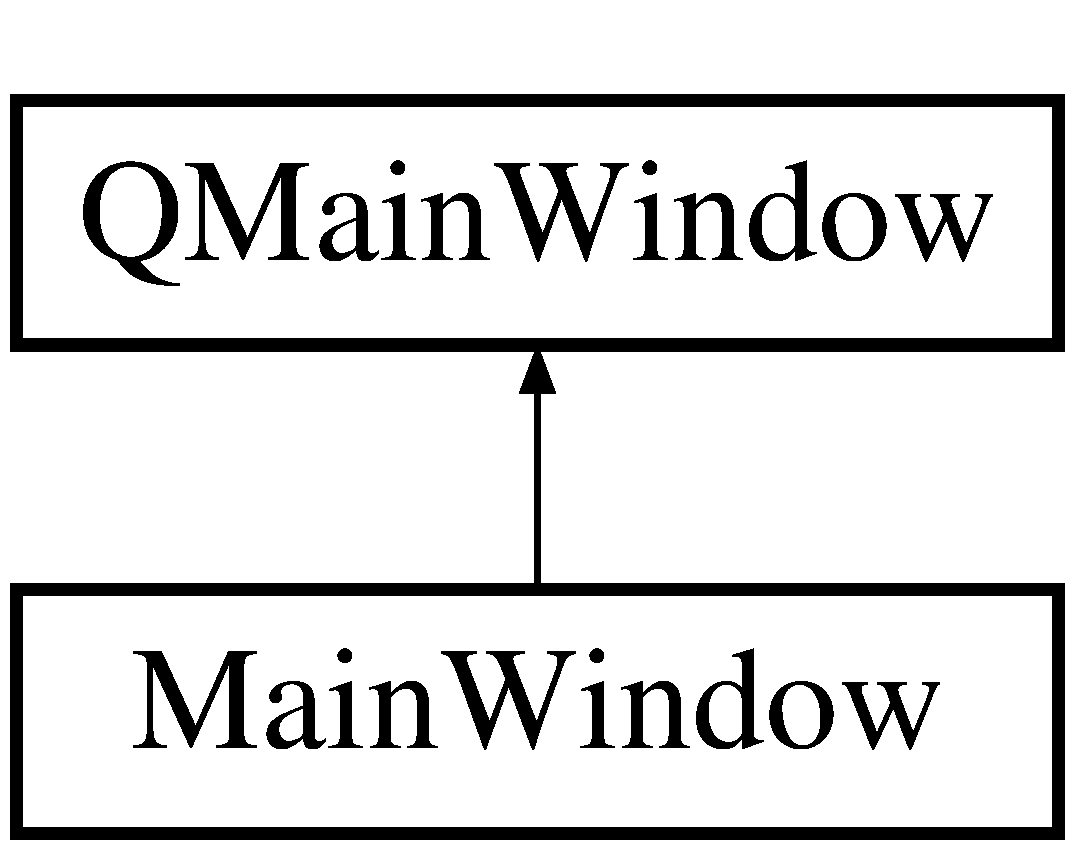
\includegraphics[height=2.000000cm]{classMainWindow}
\end{center}
\end{figure}
\subsection*{Public Member Functions}
\begin{DoxyCompactItemize}
\item 
\hyperlink{classMainWindow_a5e929afe3d79ebd9b7c48d89799308ca}{Main\-Window} (const Q\-String \&proj\-File, const Q\-String \&run\-Dir, Q\-Widget $\ast$parent=0)
\begin{DoxyCompactList}\small\item\em Constructs a Lib\-Man \hyperlink{classMainWindow}{Main\-Window} object with the given arguments. \end{DoxyCompactList}\item 
\hyperlink{classMainWindow_ae98d00a93bc118200eeef9f9bba1dba7}{$\sim$\-Main\-Window} ()
\begin{DoxyCompactList}\small\item\em Destroys the main window. \end{DoxyCompactList}\end{DoxyCompactItemize}
\subsection*{Private Types}
\begin{DoxyCompactItemize}
\item 
enum \hyperlink{classMainWindow_aacc2f9b3beef5cc127f1234c65e3c21b}{R\-E\-C\-E\-N\-T\-\_\-\-F\-I\-L\-E\-S} \{ {\bfseries P\-R\-O\-J\-\_\-\-M\-A\-X\-\_\-\-C\-O\-U\-N\-T} = 5
 \}
\begin{DoxyCompactList}\small\item\em The R\-E\-C\-E\-N\-T\-\_\-\-F\-I\-L\-E\-S enum specifies maximum number of recent project files. \end{DoxyCompactList}\item 
enum \hyperlink{classMainWindow_afed3bafbe5c97894b6661920e82526f9}{C\-O\-P\-Y\-\_\-\-S\-T\-A\-T\-E} \{ {\bfseries N\-O\-N\-E} = 1000, 
{\bfseries P\-R\-O\-J\-E\-C\-T}, 
{\bfseries G\-R\-O\-U\-P}, 
{\bfseries V\-I\-E\-W}
 \}
\begin{DoxyCompactList}\small\item\em The C\-O\-P\-Y\-\_\-\-S\-T\-A\-T\-E enum specifies different states used for coping project/group/view (library/cell/view). \end{DoxyCompactList}\end{DoxyCompactItemize}
\subsection*{Private Slots}
\begin{DoxyCompactItemize}
\item 
void \hyperlink{classMainWindow_a4e20a4a065fbb0e4d3532a45a0a91425}{close\-Event} (Q\-Close\-Event $\ast$event)
\begin{DoxyCompactList}\small\item\em This event handler is called with the given event when Qt receives a window close request for a top-\/level widget from the window system. The function is used to save the projects settings. \end{DoxyCompactList}\item 
void \hyperlink{classMainWindow_a9a11decabf7bc3f32641bc59431bee3c}{show\-View\-Menu} (const Q\-Point \&pos)
\begin{DoxyCompactList}\small\item\em Displays menu for view widget. \end{DoxyCompactList}\item 
void \hyperlink{classMainWindow_a19879440aaeb18585b7fac488e540c49}{show\-Group\-Menu} (const Q\-Point \&pos)
\begin{DoxyCompactList}\small\item\em Displays menu for group (cell) widget. \end{DoxyCompactList}\item 
void \hyperlink{classMainWindow_aefeae0de6c70fcace6f9f4b3836d8a84}{show\-Library\-Menu} (const Q\-Point \&pos)
\begin{DoxyCompactList}\small\item\em Creates and displays menu for project (library) tree widget. It is used for projects management. \end{DoxyCompactList}\item 
void \hyperlink{classMainWindow_acd00c7003f796ac714582e3238788872}{show\-Category\-Menu} (const Q\-Point \&pos)
\begin{DoxyCompactList}\small\item\em Displays menu for category widget. \end{DoxyCompactList}\item 
void \hyperlink{classMainWindow_a565b14903c7bc11126bce1307afaa2e2}{add\-New\-Group} ()
\begin{DoxyCompactList}\small\item\em Creates new group (cell) and adds it to the list widget. \end{DoxyCompactList}\item 
void \hyperlink{classMainWindow_a80f2c79d5fd4ef7c0a5cf55e5a2bdb78}{add\-New\-Project} ()
\begin{DoxyCompactList}\small\item\em Creates new project (library) and adds it to the tree widget. \end{DoxyCompactList}\item 
void \hyperlink{classMainWindow_a24f572a26e33ee7b4115efd4ab6658e9}{add\-New\-Category} ()
\begin{DoxyCompactList}\small\item\em Creates new category and adds it to the tree widget. \end{DoxyCompactList}\item 
void \hyperlink{classMainWindow_a4525ad9b4f0f3df104a1f558f653f4a0}{add\-New\-Spice\-View} ()
\begin{DoxyCompactList}\small\item\em Creates new spice model view and adds it to the list widget. \end{DoxyCompactList}\item 
void \hyperlink{classMainWindow_ab2e15383545f27e0f07fdb84e714d18e}{add\-New\-Layout\-View} ()
\begin{DoxyCompactList}\small\item\em Creates new layout view and adds it to the list widget. \end{DoxyCompactList}\item 
void \hyperlink{classMainWindow_ad3a1c8710698214361128232cbde335d}{add\-New\-Schematic\-View} ()
\begin{DoxyCompactList}\small\item\em Creates new schematic view and adds it to the list widget. \end{DoxyCompactList}\item 
void \hyperlink{classMainWindow_ae8d8ed40aae7c5b596efac98925792ee}{remove\-Selected\-View} ()
\begin{DoxyCompactList}\small\item\em Removes selected view. \end{DoxyCompactList}\item 
void \hyperlink{classMainWindow_ae91780a31e7118b44feb428b0de0dba3}{remove\-Selected\-Group} ()
\begin{DoxyCompactList}\small\item\em Removes selected group (cell). \end{DoxyCompactList}\item 
void \hyperlink{classMainWindow_aa77bfbfc58c63a5f3ce5d6f718a55a40}{remove\-Selected\-Project} ()
\begin{DoxyCompactList}\small\item\em Removes selected project (library). \end{DoxyCompactList}\item 
void \hyperlink{classMainWindow_ac091629e8f90351cc3543337aefc80ea}{remove\-Selected\-Category} ()
\begin{DoxyCompactList}\small\item\em Removes selected category. \end{DoxyCompactList}\item 
void \hyperlink{classMainWindow_a6e334fe603796652be44d5df952e0f4a}{show\-View\-Info} ()
\begin{DoxyCompactList}\small\item\em Prints view file Unix information into the \hyperlink{classMainWindow}{Main\-Window} output window. \end{DoxyCompactList}\item 
void \hyperlink{classMainWindow_a7792544db8869842840c6e4716f8cbec}{show\-Group\-Info} ()
\begin{DoxyCompactList}\small\item\em Prints group folder Unix information into the \hyperlink{classMainWindow}{Main\-Window} output window. \end{DoxyCompactList}\item 
void \hyperlink{classMainWindow_a2fbeb11fb0bbe28be62403ef732931a7}{show\-Project\-Info} ()
\begin{DoxyCompactList}\small\item\em Prints library folder Unix information into the \hyperlink{classMainWindow}{Main\-Window} output window. \end{DoxyCompactList}\item 
void \hyperlink{classMainWindow_ad63d5f418c4d55c90d63269162782ac4}{show\-Category\-Info} ()
\begin{DoxyCompactList}\small\item\em Prints category file Unix information into the \hyperlink{classMainWindow}{Main\-Window} output window. \end{DoxyCompactList}\item 
void \hyperlink{classMainWindow_a41872370d39dc3c6dc8b996d42196432}{remove\-From\-Group} ()
\begin{DoxyCompactList}\small\item\em Eliminates project from the nested group. \end{DoxyCompactList}\item 
void \hyperlink{classMainWindow_a1829103fc2661a8c1f0a2c2a730da53a}{remove\-Group\-Union} ()
\begin{DoxyCompactList}\small\item\em Delets group (nested projects) from the tree widget. \end{DoxyCompactList}\item 
void \hyperlink{classMainWindow_a38f2a589547d744fe8effcd86d56522f}{show\-Folder\-Info} (const Q\-String \&, const Q\-String \&, const Q\-String \&, bool clear=true)
\begin{DoxyCompactList}\small\item\em Prints folder Unix information into the \hyperlink{classMainWindow}{Main\-Window} output window. \end{DoxyCompactList}\item 
void \hyperlink{classMainWindow_aedcf4e7322932599339fd7213751e653}{merge\-Project\-Into\-Group} ()
\begin{DoxyCompactList}\small\item\em Merges project into a nested group. \end{DoxyCompactList}\item 
void \hyperlink{classMainWindow_a003d3ff529129c1613cabc25dcbb3450}{paste\-Selected\-Data} ()
\begin{DoxyCompactList}\small\item\em Pastes selected data (could be project, group or file. \end{DoxyCompactList}\item 
void \hyperlink{classMainWindow_a6da44654044153535dabe1cfd21714be}{copy\-Selected\-View} ()
\begin{DoxyCompactList}\small\item\em Adds selected view to the buffer for coping. \end{DoxyCompactList}\item 
void \hyperlink{classMainWindow_a0eb4ce1b63db072df36b119b0488d8ce}{copy\-Selected\-Group} ()
\begin{DoxyCompactList}\small\item\em Adds selected group to the buffer for coping. \end{DoxyCompactList}\item 
void \hyperlink{classMainWindow_a519a38c202ac69dbc0c2e5d0ae971768}{copy\-Selected\-Project} ()
\begin{DoxyCompactList}\small\item\em Copies selected project to the buffer. \end{DoxyCompactList}\item 
void \hyperlink{classMainWindow_af2fb86d1f28ac5f40c0cfdc40280b08c}{clear\-Current\-Copy\-State} ()
\begin{DoxyCompactList}\small\item\em Clears current buffer used for coping of data. \end{DoxyCompactList}\item 
void \hyperlink{classMainWindow_a5fc888265a0d9c20a6a5fc4828d3b434}{add\-View\-To\-Be\-Copied} (const Q\-String \&)
\begin{DoxyCompactList}\small\item\em Adds group to the buffer for later coping. \end{DoxyCompactList}\item 
void \hyperlink{classMainWindow_a34d6f30b3ac4af259e64a141200f49da}{add\-Project\-To\-Be\-Copied} (const Q\-String \&)
\begin{DoxyCompactList}\small\item\em Adds project to the buffer for later coping. \end{DoxyCompactList}\item 
void \hyperlink{classMainWindow_af85f171e5a269a87031d100455b78b82}{add\-Group\-To\-Be\-Copied} (const Q\-String \&, const Q\-String \&)
\begin{DoxyCompactList}\small\item\em Adds group to the buffer for later coping. \end{DoxyCompactList}\item 
void \hyperlink{classMainWindow_aad64417dd963cf8816a47097df343297}{load\-Recent\-Project} ()
\begin{DoxyCompactList}\small\item\em Loads the most recent project file into Lib\-Man environment. \end{DoxyCompactList}\item 
void \hyperlink{classMainWindow_ad8c228fb00728ea101b53f2778c96a1a}{update\-Recent\-Project\-Actions} ()
\begin{DoxyCompactList}\small\item\em Updates File-\/$>$Recent menu items. \end{DoxyCompactList}\item 
void \hyperlink{classMainWindow_a0b51bc62adc32da1189785375d888595}{load\-Project\-File} (const Q\-String \&)
\begin{DoxyCompactList}\small\item\em Loads project file contence into Lib\-Man. \end{DoxyCompactList}\item 
void \hyperlink{classMainWindow_a8513c227af4759727cdaff0528760411}{save\-Project\-File} (const Q\-String \&)
\begin{DoxyCompactList}\small\item\em Saves Lib\-Man Library/\-Cell/\-View data into project file. \end{DoxyCompactList}\item 
void \hyperlink{classMainWindow_aafa974e05a80e493c719909da5e5b76d}{set\-Recent\-Project} (const Q\-String \&)
\begin{DoxyCompactList}\small\item\em Sets the name of the last loaded project to the upper recent file list. \end{DoxyCompactList}\item 
void \hyperlink{classMainWindow_ad550c61cfa05c7e528dedc6cf636ed10}{on\-\_\-action\-Save\-\_\-triggered} ()
\begin{DoxyCompactList}\small\item\em Saves the current project file or executes on\-\_\-action\-Save\-\_\-\-As\-\_\-triggered if no current file specified. \end{DoxyCompactList}\item 
void \hyperlink{classMainWindow_a98e86ef6104b6e2910328af2f878438d}{on\-\_\-action\-Save\-\_\-\-As\-\_\-triggered} ()
\begin{DoxyCompactList}\small\item\em Pops up dialog box where user can specify the file to save the project libraries. \end{DoxyCompactList}\item 
void \hyperlink{classMainWindow_ab4487c4b02224acd4a0193d38b704ddb}{on\-\_\-action\-Exit\-\_\-triggered} ()
\begin{DoxyCompactList}\small\item\em Closes Lib\-Man. \end{DoxyCompactList}\item 
void \hyperlink{classMainWindow_ad1c8aa9c6519123e3f314c84d46a8317}{on\-\_\-action\-Show\-\_\-\-Categories\-\_\-toggled} (bool)
\begin{DoxyCompactList}\small\item\em Slot is triggered to show or hide the categories tree widget. \end{DoxyCompactList}\item 
void \hyperlink{classMainWindow_adc9158772dde195daaa1d04276d6889a}{on\-\_\-action\-Show\-\_\-\-Documents\-\_\-toggled} (bool)
\begin{DoxyCompactList}\small\item\em Slot is triggered to show or hide the documentation tree widget. \end{DoxyCompactList}\item 
void \hyperlink{classMainWindow_afd40b73a712b16f9c77dd029024b75ce}{on\-\_\-action\-Tools\-\_\-triggered} ()
\begin{DoxyCompactList}\small\item\em Triggers execution of \hyperlink{classToolManager}{Tool\-Manager} dialog window. \end{DoxyCompactList}\item 
void \hyperlink{classMainWindow_aa1d84c313076357330d8f2f9c0b0b96d}{on\-\_\-action\-Projects\-\_\-triggered} ()
\begin{DoxyCompactList}\small\item\em Triggers execution of \hyperlink{classProjectManager}{Project\-Manager} dialog window. \end{DoxyCompactList}\item 
void \hyperlink{classMainWindow_a48ed0a16f674e38e0e2a24274852a9af}{on\-\_\-action\-Open\-\_\-triggered} ()
\begin{DoxyCompactList}\small\item\em Launches a dialog window to select a project file to load. \end{DoxyCompactList}\item 
void \hyperlink{classMainWindow_a00f1c23c161a4384060fc8ee682e76ba}{on\-\_\-action\-Clear\-\_\-\-Recent\-\_\-\-File\-\_\-\-Stack\-\_\-triggered} ()
\begin{DoxyCompactList}\small\item\em Removes all the project file items from the menu. \end{DoxyCompactList}\item 
void \hyperlink{classMainWindow_a6559de64b12cdf8254275d87a4babc0a}{on\-\_\-tree\-Libs\-\_\-item\-Clicked} (Q\-Tree\-Widget\-Item $\ast$item, int column)
\begin{DoxyCompactList}\small\item\em Slot to load all groups (cells) for selected project (library) into the group (cell) list widget. \end{DoxyCompactList}\item 
void \hyperlink{classMainWindow_ad95e75085713bdbfa441172f267e7ea2}{on\-\_\-list\-Groups\-\_\-item\-Clicked} (Q\-List\-Widget\-Item $\ast$item)
\begin{DoxyCompactList}\small\item\em Slot to load all views for selected group (cell) into the view list widget. \end{DoxyCompactList}\item 
void \hyperlink{classMainWindow_a56d68978d07e45cffe0d6d925b647744}{on\-\_\-list\-Views\-\_\-item\-Double\-Clicked} (Q\-List\-Widget\-Item $\ast$item)
\begin{DoxyCompactList}\small\item\em Slot to execute a tool based on the selected item (schematic, layout, cdl, spice, etc.). \end{DoxyCompactList}\item 
void \hyperlink{classMainWindow_aca2a1d9becfed505821bb7e7a945d5b5}{on\-\_\-list\-Documentation\-\_\-item\-Double\-Clicked} (Q\-Tree\-Widget\-Item $\ast$item)
\begin{DoxyCompactList}\small\item\em Slot is to execute document viewer with specified documentation. \end{DoxyCompactList}\item 
void \hyperlink{classMainWindow_a466c34043cd652304aa4e7e0e31ccf0f}{on\-\_\-list\-Views\-\_\-item\-Clicked} (Q\-List\-Widget\-Item $\ast$item)
\begin{DoxyCompactList}\small\item\em Sets the name of the selected item into the view filter line edit. \end{DoxyCompactList}\item 
void \hyperlink{classMainWindow_ab6bac75e491c0ff6399d8761a4d9b291}{on\-\_\-list\-Categories\-\_\-item\-Clicked} (Q\-Tree\-Widget\-Item $\ast$item)
\begin{DoxyCompactList}\small\item\em Slot is to load groups (cells) located into the specified category file. \end{DoxyCompactList}\item 
void \hyperlink{classMainWindow_a53c77b4bec2f9f9e5ee2a9f3c1100caf}{on\-\_\-tree\-Libs\-\_\-item\-Changed} (Q\-Tree\-Widget\-Item $\ast$item, int column)
\begin{DoxyCompactList}\small\item\em Slot is triggered when tree item is changed. Used for storing the project names after renaming. \end{DoxyCompactList}\item 
void \hyperlink{classMainWindow_aa829e818519a2d617c78b3e832e3a4ea}{on\-\_\-list\-Categories\-\_\-item\-Double\-Clicked} (Q\-Tree\-Widget\-Item $\ast$item, int column)
\begin{DoxyCompactList}\small\item\em Slot to execute a tool to view ctegory content. \end{DoxyCompactList}\item 
void \hyperlink{classMainWindow_a3d411ebea0a66c65174a7918a5317881}{on\-\_\-txt\-Lib\-Search\-\_\-text\-Edited} (const Q\-String \&arg1)
\begin{DoxyCompactList}\small\item\em Filters projects (libraries) based on user input. \end{DoxyCompactList}\item 
void \hyperlink{classMainWindow_ab678d8f29e983817bedf692d399f8f22}{on\-\_\-txt\-Cat\-Search\-\_\-text\-Edited} (const Q\-String \&arg1)
\begin{DoxyCompactList}\small\item\em Filters categories based on user input. \end{DoxyCompactList}\item 
void \hyperlink{classMainWindow_aa083f16ffe18dc0d31fabece8d9decff}{on\-\_\-txt\-Cell\-Search\-\_\-text\-Edited} (const Q\-String \&arg1)
\begin{DoxyCompactList}\small\item\em Filters groups (cells) based on user input. \end{DoxyCompactList}\item 
void \hyperlink{classMainWindow_a468a4eb5ab08b6472e6c32b35490aeeb}{on\-\_\-txt\-View\-Search\-\_\-text\-Edited} (const Q\-String \&arg1)
\begin{DoxyCompactList}\small\item\em Filters views based on user input. \end{DoxyCompactList}\item 
void \hyperlink{classMainWindow_a4f3ebda1ba39e0ef4d678b44893c9c7f}{on\-\_\-action\-About\-\_\-triggered} ()
\begin{DoxyCompactList}\small\item\em Triggers execution of \hyperlink{classAbout}{About} dialog window. \end{DoxyCompactList}\item 
void \hyperlink{classMainWindow_a72557ed75b052bdf4f7f8d87b70fc579}{on\-\_\-action\-Project\-\_\-triggered} ()
\begin{DoxyCompactList}\small\item\em Triggers creation of new project (library). \end{DoxyCompactList}\item 
void \hyperlink{classMainWindow_a9a3efa0112bdda7a589525d160ca625b}{on\-\_\-action\-Group\-\_\-triggered} ()
\begin{DoxyCompactList}\small\item\em Triggers creation of new group (cell). \end{DoxyCompactList}\item 
void \hyperlink{classMainWindow_ab7c8299c50bb97eaedcb225e90f9bcf4}{on\-\_\-action\-Union\-\_\-triggered} ()
\begin{DoxyCompactList}\small\item\em Triggers execution of \hyperlink{classNewView}{New\-View} dialog window. \end{DoxyCompactList}\item 
void \hyperlink{classMainWindow_a2812d2f0350ea5a0da583953fa25b19f}{on\-\_\-action\-Category\-\_\-triggered} ()
\begin{DoxyCompactList}\small\item\em Triggers creation of new category. \end{DoxyCompactList}\item 
void \hyperlink{classMainWindow_a541e1460680230409808d47585c4b8b4}{on\-\_\-action\-Session\-\_\-triggered} ()
\begin{DoxyCompactList}\small\item\em Creates new session and clears up all current project settings. \end{DoxyCompactList}\end{DoxyCompactItemize}
\subsection*{Private Member Functions}
\begin{DoxyCompactItemize}
\item 
void \hyperlink{classMainWindow_a9bb1f3b7f6b5360abfd2dc01fc1c8930}{load\-Settings} ()
\begin{DoxyCompactList}\small\item\em Loads Lib\-Man settings (geometry, tools, widget states etc.) and aplies them accordingly. \end{DoxyCompactList}\item 
void \hyperlink{classMainWindow_adc87dcfb242d83a35794e011f8c29e41}{info} (const Q\-String \&msg, bool clear=true)
\begin{DoxyCompactList}\small\item\em Displays basic message in the output text widget of Lib\-Man. \end{DoxyCompactList}\item 
void \hyperlink{classMainWindow_aa3bc340f4289a4ef73e5feaa6c5b1a9a}{error} (const Q\-String \&msg, bool clear=true)
\begin{DoxyCompactList}\small\item\em Displays error message in the output text widget of Lib\-Man. \end{DoxyCompactList}\item 
void \hyperlink{classMainWindow_a5459d4fe95a19b1cf74aef261168c31d}{init\-Recent\-Project\-Menu} ()
\begin{DoxyCompactList}\small\item\em Initializes recent menu and assigns menu items with assotiated project files. \end{DoxyCompactList}\item 
bool \hyperlink{classMainWindow_a0045ab02ba4ef6bb3d777236983219bc}{create\-New\-File} (const Q\-String \&)
\begin{DoxyCompactList}\small\item\em Creates an empty project file. \end{DoxyCompactList}\item 
bool \hyperlink{classMainWindow_ab01cf882613a0b0ea2a35700be933143}{is\-State\-Changed} () const 
\begin{DoxyCompactList}\small\item\em Returns true the Lib\-Man window state has been changed, otherwise false. \end{DoxyCompactList}\item 
void \hyperlink{classMainWindow_a5fb61a8cf4108faeb224c8f2d99b6ee3}{set\-State\-Saved} ()
\begin{DoxyCompactList}\small\item\em Set Lib\-Man state saved and updates the window titel accordingly. \end{DoxyCompactList}\item 
void \hyperlink{classMainWindow_a281bfe571e3ce2af52bf79bb4fa44fde}{set\-State\-Changed} ()
\begin{DoxyCompactList}\small\item\em Set Lib\-Man state changed and updates the window titel accordingly. \end{DoxyCompactList}\item 
void \hyperlink{classMainWindow_a8c2508cb0a54eab87a3c5c5471676f4a}{check\-And\-Save\-Project\-Data} (Q\-Close\-Event $\ast$)
\begin{DoxyCompactList}\small\item\em If state of the Lib\-Man has been changed the dialog window pops up to ask user for saving of the changes. \end{DoxyCompactList}\item 
void \hyperlink{classMainWindow_aff15de0c74551acef80d0a588c254b7e}{create\-Project\-Union\-Menu} ()
\begin{DoxyCompactList}\small\item\em Creates and displays menu for project group (nested projects). \end{DoxyCompactList}\item 
void \hyperlink{classMainWindow_a63962c76c33dd60e0b354dd48724a9f5}{load\-Libraries} ()
\begin{DoxyCompactList}\small\item\em Adds project (libraries) into the project tree widget from the Lib\-Man settings. \end{DoxyCompactList}\item 
void \hyperlink{classMainWindow_a57bf47c514d40fcbc2cc301599fd419e}{load\-Groups} (const Q\-String \&lib\-Path)
\begin{DoxyCompactList}\small\item\em Adds group (cell) for the given project (library) into the group list widget. \end{DoxyCompactList}\item 
void \hyperlink{classMainWindow_a953304e2b85e660d11bb875f5e9f3738}{load\-Documents} (const Q\-String \&lib\-Path)
\begin{DoxyCompactList}\small\item\em Adds documents for the given project (library) into the document tree widget. \end{DoxyCompactList}\item 
void \hyperlink{classMainWindow_a75030b8780aaa7a2a1f44af3ae72feed}{load\-Categories} (const Q\-String \&lib\-Path)
\begin{DoxyCompactList}\small\item\em Adds categories for the given project (library) into the category tree widget. \end{DoxyCompactList}\item 
void \hyperlink{classMainWindow_a5ebd5eb51726eb69e0e0243750c926a9}{load\-Combined\-Libs} (const Q\-Map$<$ Q\-String, Q\-String\-List $>$ \&)
\begin{DoxyCompactList}\small\item\em Adds given nested projects (libraries) into the project tree widget. \end{DoxyCompactList}\item 
void \hyperlink{classMainWindow_a4124c5b7d11a382c1d131b93787d397a}{load\-Views} (const Q\-String \&lib\-Path, const Q\-String \&group\-Name)
\begin{DoxyCompactList}\small\item\em Adds views for the given group (cell) into the view list widget. \end{DoxyCompactList}\item 
void \hyperlink{classMainWindow_a4d19d583bbd0cdfe6db28d7253e98c69}{hide\-Tree\-Item} (Q\-Tree\-Widget $\ast$, const Q\-String \&filter)
\begin{DoxyCompactList}\small\item\em Hides tree item during filtering. \end{DoxyCompactList}\item 
void \hyperlink{classMainWindow_afd7b30dc6f95760354af27809bc86a53}{hide\-List\-Item} (Q\-List\-Widget $\ast$, const Q\-String \&filter)
\begin{DoxyCompactList}\small\item\em Hides list item during filtering. \end{DoxyCompactList}\item 
bool \hyperlink{classMainWindow_a477c0c286505480fa0ecab597cc928aa}{is\-View\-Copied} () const 
\begin{DoxyCompactList}\small\item\em Returns true the Lib\-Man view state has been changed, otherwise false. \end{DoxyCompactList}\item 
bool \hyperlink{classMainWindow_a2b97dc2343a874c73c6c8453c89a98ae}{is\-Group\-Copied} () const 
\begin{DoxyCompactList}\small\item\em Returns true the Lib\-Man group (cell) state has been changed, otherwise false. \end{DoxyCompactList}\item 
bool \hyperlink{classMainWindow_a35f6e8e6d58371d363fcb7fc199e86ba}{is\-Project\-Copied} () const 
\begin{DoxyCompactList}\small\item\em Returns true the Lib\-Man project (library) state has been changed, otherwise false. \end{DoxyCompactList}\item 
bool \hyperlink{classMainWindow_a6cc24c7cd36704cdf570e26b5621fc66}{ask\-For\-File\-Replacement} () const 
\begin{DoxyCompactList}\small\item\em Displays a dialog box to confirm file replacement. \end{DoxyCompactList}\item 
bool \hyperlink{classMainWindow_afbea101d81d3423e32bcd200f6dd7c39}{ask\-For\-Permanent\-Delete} () const 
\begin{DoxyCompactList}\small\item\em Displays a dialog box to confirm permanent removing of file. \end{DoxyCompactList}\item 
bool \hyperlink{classMainWindow_a380a7f848e6a3b97d21d94643e02c046}{ask\-User\-For\-Action} (const Q\-String \&title) const 
\begin{DoxyCompactList}\small\item\em Displays a dialog box to confirm user action. For ex., removing folder or file. \end{DoxyCompactList}\item 
bool \hyperlink{classMainWindow_a488161a7ea31be35bf87091772c5a235}{remove\-Dir} (const Q\-String \&) const 
\begin{DoxyCompactList}\small\item\em Deletes folder recursevly. \end{DoxyCompactList}\item 
void \hyperlink{classMainWindow_a9a8e06194b0035c089c872646b5cb4b6}{copy\-Dir} (const Q\-String \&, const Q\-String \&) const 
\begin{DoxyCompactList}\small\item\em Copies folder recursevly. \end{DoxyCompactList}\item 
Q\-String \hyperlink{classMainWindow_aa4dfdf9b2b26f558e0edcd10604d7607}{get\-Library\-Path} (const Q\-String \&) const 
\begin{DoxyCompactList}\small\item\em Returns library path based on the project (library) name. \end{DoxyCompactList}\item 
Q\-String \hyperlink{classMainWindow_a651742fa870b7fd7ec990f12f5f385d7}{get\-Library\-Key\-Prefix} () const 
\begin{DoxyCompactList}\small\item\em Returns prefix for storing libraries in the Lib\-Man settings collection. \end{DoxyCompactList}\item 
Q\-String \hyperlink{classMainWindow_a731c741711ec82b6d0d83e80850aaa33}{get\-Project\-File\-From\-Dir} (const Q\-String \&) const 
\begin{DoxyCompactList}\small\item\em Searches for $\ast$.projects-\/files in the specified directory and returns the first found one. \end{DoxyCompactList}\item 
Q\-String \hyperlink{classMainWindow_a3a8c2f752b4590008e2d729aa215045d}{generate\-Copy\-Name} (const Q\-String \&, const Q\-String \&, const Q\-String \&suffix=\char`\"{}\char`\"{}) const 
\begin{DoxyCompactList}\small\item\em Generates unexisting name based on the given information. Used when coping an item. \end{DoxyCompactList}\item 
Q\-String \hyperlink{classMainWindow_a644755d8ccb3af92b9219b7c93920afd}{get\-View\-Path} (const Q\-String \&, const Q\-String \&, const Q\-String \&) const 
\begin{DoxyCompactList}\small\item\em Returns absolute path of the view based on given project/group/view (library/cell/view) information. \end{DoxyCompactList}\item 
Q\-String \hyperlink{classMainWindow_a43a1dca579bdf54ec0728022ba5bcef4}{get\-Current\-View\-Name} () const 
\begin{DoxyCompactList}\small\item\em Returns currently selected view name. \end{DoxyCompactList}\item 
Q\-String \hyperlink{classMainWindow_ab7deaf83db422f4124d9e48f6b950278}{get\-Current\-Group\-Name} () const 
\begin{DoxyCompactList}\small\item\em Returns currently selected group (cell) name. \end{DoxyCompactList}\item 
Q\-String \hyperlink{classMainWindow_a3ad77a7c895c3a37cb022d124057c5e8}{get\-Current\-Union\-Name} () const 
\begin{DoxyCompactList}\small\item\em Returns currently selected project union (nested projects) name. \end{DoxyCompactList}\item 
Q\-String \hyperlink{classMainWindow_a122007410ead45d63e205e4aa612ac77}{get\-Current\-Working\-Dir} () const 
\begin{DoxyCompactList}\small\item\em Returns current working directory from where the project file has been loaded, otherwise user home path. \end{DoxyCompactList}\item 
Q\-String \hyperlink{classMainWindow_afae5dfaa6de8707fde2c2cc530a462b4}{get\-Current\-Library\-Name} () const 
\begin{DoxyCompactList}\small\item\em Returns currently selected project (library) name. \end{DoxyCompactList}\item 
Q\-String \hyperlink{classMainWindow_a0cb5632672f6e9f8091fcbb6ed7d8614}{get\-Current\-Project\-File} () const 
\begin{DoxyCompactList}\small\item\em Returns path to the current project file. \end{DoxyCompactList}\item 
Q\-String \hyperlink{classMainWindow_a2db5fde30507e1eb136ef3eeb17307dc}{get\-Current\-Library\-Path} () const 
\begin{DoxyCompactList}\small\item\em Returns absolute path of the currently selected project (library) \end{DoxyCompactList}\item 
Q\-String \hyperlink{classMainWindow_adf5753c529cbbe719f41d2fb456e7cea}{get\-Current\-Category\-Name} () const 
\begin{DoxyCompactList}\small\item\em Returns currently selected name of category. \end{DoxyCompactList}\item 
Q\-String \hyperlink{classMainWindow_a603c56475b8ef3f6eb34ad8396abfbea}{get\-Current\-View\-File\-Path} (const Q\-String \&) const 
\begin{DoxyCompactList}\small\item\em Returns absolute path of the view for currently selected project/group (library/cell). \end{DoxyCompactList}\item 
Q\-String \hyperlink{classMainWindow_aa821e37fd6ba03b3e920e3bcf9290f56}{get\-Current\-Document\-File\-Path} (const Q\-String \&) const 
\begin{DoxyCompactList}\small\item\em Returns absolute documentation file path based on the given library path and document name. \end{DoxyCompactList}\item 
Q\-String \hyperlink{classMainWindow_a627010ec88cbfea1f08d7eb828df8497}{get\-Current\-Group\-Path} (const Q\-String \&view\-Name, bool to\-Be\-Created=false)
\begin{DoxyCompactList}\small\item\em \hyperlink{classMainWindow_a627010ec88cbfea1f08d7eb828df8497}{Main\-Window\-::get\-Current\-Group\-Path}. \end{DoxyCompactList}\item 
Q\-String \hyperlink{classMainWindow_ad191fe52bbc3ce40d18fb61f5655e562}{get\-Settings\-Header\-Name} () const 
\begin{DoxyCompactList}\small\item\em Returns header name used for storing Lib\-Man settings. \end{DoxyCompactList}\item 
Q\-String \hyperlink{classMainWindow_a37460aa0e52d6f1f7e4141824d371946}{get\-Tool\-By\-View} (const Q\-String \&) const 
\begin{DoxyCompactList}\small\item\em Returns specified by user tool for displaying views based on view name. \end{DoxyCompactList}\item 
Q\-String \hyperlink{classMainWindow_a1454fa08837579178f9a561675950f13}{get\-Document\-Tool} (const Q\-String \&) const 
\begin{DoxyCompactList}\small\item\em Returns specified by user tool for viewing documents based on doument name. \end{DoxyCompactList}\item 
Q\-String \hyperlink{classMainWindow_a4cf32e9db205b35bec796aeb55d2759a}{get\-Lib\-Man\-Title} () const 
\begin{DoxyCompactList}\small\item\em Returns titel of the Lib\-Man. \end{DoxyCompactList}\item 
Q\-String\-List \hyperlink{classMainWindow_a2e94b321482f5d6a970f0924f74859a3}{get\-Valid\-View\-List} () const 
\begin{DoxyCompactList}\small\item\em Returns list of valid view names. \end{DoxyCompactList}\item 
Q\-String\-List \hyperlink{classMainWindow_aadfbacf644193df620f494f5bf8106be}{get\-Current\-Groups} (const Q\-String \&) const 
\begin{DoxyCompactList}\small\item\em Returns project group (cell) list. \end{DoxyCompactList}\item 
Q\-String\-List \hyperlink{classMainWindow_a31c68c1e82618ac86398afd52f58c04e}{get\-Current\-Views} (const Q\-String \&, const Q\-String \&) const 
\begin{DoxyCompactList}\small\item\em Returns valid view paths for the carent project/ group (library/cell). \end{DoxyCompactList}\item 
Q\-String\-List \hyperlink{classMainWindow_a5f419797d8b22ee1c713e841931a23a4}{read\-Library\-Categories} (const Q\-String \&, const Q\-String \&)
\begin{DoxyCompactList}\small\item\em Reads library category and returns it's cells. \end{DoxyCompactList}\item 
Q\-Tree\-Widget\-Item $\ast$ \hyperlink{classMainWindow_ae23d791628eb7fb2d9edf8ee0649113c}{get\-Tree\-Item\-By\-Name} (const Q\-String \&name)
\begin{DoxyCompactList}\small\item\em Returns pointer to tree item. \end{DoxyCompactList}\item 
Q\-Map$<$ Q\-String, Q\-String $>$ \hyperlink{classMainWindow_ac6106cd3a58bfc4453ada97dd49cff63}{get\-Current\-Libraries} () const 
\begin{DoxyCompactList}\small\item\em Returns list of the currently loaded projects (libraries). \end{DoxyCompactList}\end{DoxyCompactItemize}
\subsection*{Private Attributes}
\begin{DoxyCompactItemize}
\item 
Ui\-::\-Main\-Window $\ast$ \hyperlink{classMainWindow_a5a3eb262660797d9a4d52ed16edb6d11}{m\-\_\-ui}
\item 
\hyperlink{classProperties}{Properties} $\ast$ \hyperlink{classMainWindow_a22f004bec556234a5eb739cfa1819647}{m\-\_\-properties}
\item 
bool \hyperlink{classMainWindow_a3c61f9d7deec39afb315e57ef159ba18}{m\-\_\-is\-State\-Changed}
\item 
Q\-String \hyperlink{classMainWindow_a494664d1901f3d94237411b34e7a2a16}{m\-\_\-item\-Text}
\item 
Q\-String \hyperlink{classMainWindow_a9294c8737725afe7b0b7dcc311881959}{m\-\_\-run\-Directory}
\item 
Q\-String \hyperlink{classMainWindow_ade3f7ebe5eb1bf67444cd41b2bc38aca}{m\-\_\-current\-Proj\-File}
\item 
Q\-List$<$ Q\-Action $\ast$ $>$ \hyperlink{classMainWindow_a4135ecd5a58b2679333740dddc8d2cf8}{m\-\_\-recent\-Projects}
\item 
Q\-String\-List \hyperlink{classMainWindow_a306adca5f257e5aeaa50ff06605a7a86}{m\-\_\-copy\-Data}
\item 
\hyperlink{classMainWindow_afed3bafbe5c97894b6661920e82526f9}{C\-O\-P\-Y\-\_\-\-S\-T\-A\-T\-E} \hyperlink{classMainWindow_a77153a35340c4a8a40f8528301bd96ad}{m\-\_\-current\-Copy\-State}
\end{DoxyCompactItemize}
\subsection*{Friends}
\begin{DoxyCompactItemize}
\item 
\hypertarget{classMainWindow_a132813282374dcbc6788609035b58c5a}{class {\bfseries New\-View}}\label{classMainWindow_a132813282374dcbc6788609035b58c5a}

\item 
\hypertarget{classMainWindow_aa860c957116c15c1b786357fbcd19fc7}{class {\bfseries Project\-Manager}}\label{classMainWindow_aa860c957116c15c1b786357fbcd19fc7}

\end{DoxyCompactItemize}


\subsection{Detailed Description}
The \hyperlink{classMainWindow}{Main\-Window} class is responsible for creating main framework of Lib\-Man and controlls all slots and signals. 



 

\subsection{Constructor \& Destructor Documentation}
\hypertarget{classMainWindow_a5e929afe3d79ebd9b7c48d89799308ca}{\index{Main\-Window@{Main\-Window}!Main\-Window@{Main\-Window}}
\index{Main\-Window@{Main\-Window}!MainWindow@{Main\-Window}}
\subsubsection[{Main\-Window}]{\setlength{\rightskip}{0pt plus 5cm}Main\-Window\-::\-Main\-Window (
\begin{DoxyParamCaption}
\item[{const Q\-String \&}]{proj\-File, }
\item[{const Q\-String \&}]{run\-Dir, }
\item[{Q\-Widget $\ast$}]{parent = {\ttfamily 0}}
\end{DoxyParamCaption}
)\hspace{0.3cm}{\ttfamily [explicit]}}}\label{classMainWindow_a5e929afe3d79ebd9b7c48d89799308ca}


Constructs a Lib\-Man \hyperlink{classMainWindow}{Main\-Window} object with the given arguments. 



 
\begin{DoxyParams}{Parameters}
{\em proj\-File} & Path to the project file. Be default, it will be searched in the current folder. \\
\hline
{\em run\-Dir} & Path to the directory, where application was executed. \\
\hline
{\em parent} & Parent widget, by default is N\-U\-L\-L. \\
\hline
\end{DoxyParams}
\hypertarget{classMainWindow_ae98d00a93bc118200eeef9f9bba1dba7}{\index{Main\-Window@{Main\-Window}!$\sim$\-Main\-Window@{$\sim$\-Main\-Window}}
\index{$\sim$\-Main\-Window@{$\sim$\-Main\-Window}!MainWindow@{Main\-Window}}
\subsubsection[{$\sim$\-Main\-Window}]{\setlength{\rightskip}{0pt plus 5cm}Main\-Window\-::$\sim$\-Main\-Window (
\begin{DoxyParamCaption}
{}
\end{DoxyParamCaption}
)}}\label{classMainWindow_ae98d00a93bc118200eeef9f9bba1dba7}


Destroys the main window. 



 

\subsection{Member Function Documentation}
\hypertarget{classMainWindow_af85f171e5a269a87031d100455b78b82}{\index{Main\-Window@{Main\-Window}!add\-Group\-To\-Be\-Copied@{add\-Group\-To\-Be\-Copied}}
\index{add\-Group\-To\-Be\-Copied@{add\-Group\-To\-Be\-Copied}!MainWindow@{Main\-Window}}
\subsubsection[{add\-Group\-To\-Be\-Copied}]{\setlength{\rightskip}{0pt plus 5cm}void Main\-Window\-::add\-Group\-To\-Be\-Copied (
\begin{DoxyParamCaption}
\item[{const Q\-String \&}]{group\-Name, }
\item[{const Q\-String \&}]{group\-Path}
\end{DoxyParamCaption}
)\hspace{0.3cm}{\ttfamily [private]}, {\ttfamily [slot]}}}\label{classMainWindow_af85f171e5a269a87031d100455b78b82}


Adds group to the buffer for later coping. 



 
\begin{DoxyParams}{Parameters}
{\em group\-Name} & Name of the group to copy. \\
\hline
{\em group\-Path} & Path of the group from where to copy. \\
\hline
\end{DoxyParams}
\hypertarget{classMainWindow_a24f572a26e33ee7b4115efd4ab6658e9}{\index{Main\-Window@{Main\-Window}!add\-New\-Category@{add\-New\-Category}}
\index{add\-New\-Category@{add\-New\-Category}!MainWindow@{Main\-Window}}
\subsubsection[{add\-New\-Category}]{\setlength{\rightskip}{0pt plus 5cm}void Main\-Window\-::add\-New\-Category (
\begin{DoxyParamCaption}
{}
\end{DoxyParamCaption}
)\hspace{0.3cm}{\ttfamily [private]}, {\ttfamily [slot]}}}\label{classMainWindow_a24f572a26e33ee7b4115efd4ab6658e9}


Creates new category and adds it to the tree widget. 



 \hypertarget{classMainWindow_a565b14903c7bc11126bce1307afaa2e2}{\index{Main\-Window@{Main\-Window}!add\-New\-Group@{add\-New\-Group}}
\index{add\-New\-Group@{add\-New\-Group}!MainWindow@{Main\-Window}}
\subsubsection[{add\-New\-Group}]{\setlength{\rightskip}{0pt plus 5cm}void Main\-Window\-::add\-New\-Group (
\begin{DoxyParamCaption}
{}
\end{DoxyParamCaption}
)\hspace{0.3cm}{\ttfamily [private]}, {\ttfamily [slot]}}}\label{classMainWindow_a565b14903c7bc11126bce1307afaa2e2}


Creates new group (cell) and adds it to the list widget. 



 \hypertarget{classMainWindow_ab2e15383545f27e0f07fdb84e714d18e}{\index{Main\-Window@{Main\-Window}!add\-New\-Layout\-View@{add\-New\-Layout\-View}}
\index{add\-New\-Layout\-View@{add\-New\-Layout\-View}!MainWindow@{Main\-Window}}
\subsubsection[{add\-New\-Layout\-View}]{\setlength{\rightskip}{0pt plus 5cm}void Main\-Window\-::add\-New\-Layout\-View (
\begin{DoxyParamCaption}
{}
\end{DoxyParamCaption}
)\hspace{0.3cm}{\ttfamily [private]}, {\ttfamily [slot]}}}\label{classMainWindow_ab2e15383545f27e0f07fdb84e714d18e}


Creates new layout view and adds it to the list widget. 



 \hypertarget{classMainWindow_a80f2c79d5fd4ef7c0a5cf55e5a2bdb78}{\index{Main\-Window@{Main\-Window}!add\-New\-Project@{add\-New\-Project}}
\index{add\-New\-Project@{add\-New\-Project}!MainWindow@{Main\-Window}}
\subsubsection[{add\-New\-Project}]{\setlength{\rightskip}{0pt plus 5cm}void Main\-Window\-::add\-New\-Project (
\begin{DoxyParamCaption}
{}
\end{DoxyParamCaption}
)\hspace{0.3cm}{\ttfamily [private]}, {\ttfamily [slot]}}}\label{classMainWindow_a80f2c79d5fd4ef7c0a5cf55e5a2bdb78}


Creates new project (library) and adds it to the tree widget. 



 \hypertarget{classMainWindow_ad3a1c8710698214361128232cbde335d}{\index{Main\-Window@{Main\-Window}!add\-New\-Schematic\-View@{add\-New\-Schematic\-View}}
\index{add\-New\-Schematic\-View@{add\-New\-Schematic\-View}!MainWindow@{Main\-Window}}
\subsubsection[{add\-New\-Schematic\-View}]{\setlength{\rightskip}{0pt plus 5cm}void Main\-Window\-::add\-New\-Schematic\-View (
\begin{DoxyParamCaption}
{}
\end{DoxyParamCaption}
)\hspace{0.3cm}{\ttfamily [private]}, {\ttfamily [slot]}}}\label{classMainWindow_ad3a1c8710698214361128232cbde335d}


Creates new schematic view and adds it to the list widget. 



 \hypertarget{classMainWindow_a4525ad9b4f0f3df104a1f558f653f4a0}{\index{Main\-Window@{Main\-Window}!add\-New\-Spice\-View@{add\-New\-Spice\-View}}
\index{add\-New\-Spice\-View@{add\-New\-Spice\-View}!MainWindow@{Main\-Window}}
\subsubsection[{add\-New\-Spice\-View}]{\setlength{\rightskip}{0pt plus 5cm}void Main\-Window\-::add\-New\-Spice\-View (
\begin{DoxyParamCaption}
{}
\end{DoxyParamCaption}
)\hspace{0.3cm}{\ttfamily [private]}, {\ttfamily [slot]}}}\label{classMainWindow_a4525ad9b4f0f3df104a1f558f653f4a0}


Creates new spice model view and adds it to the list widget. 



 \hypertarget{classMainWindow_a34d6f30b3ac4af259e64a141200f49da}{\index{Main\-Window@{Main\-Window}!add\-Project\-To\-Be\-Copied@{add\-Project\-To\-Be\-Copied}}
\index{add\-Project\-To\-Be\-Copied@{add\-Project\-To\-Be\-Copied}!MainWindow@{Main\-Window}}
\subsubsection[{add\-Project\-To\-Be\-Copied}]{\setlength{\rightskip}{0pt plus 5cm}void Main\-Window\-::add\-Project\-To\-Be\-Copied (
\begin{DoxyParamCaption}
\item[{const Q\-String \&}]{proj\-Name}
\end{DoxyParamCaption}
)\hspace{0.3cm}{\ttfamily [private]}, {\ttfamily [slot]}}}\label{classMainWindow_a34d6f30b3ac4af259e64a141200f49da}


Adds project to the buffer for later coping. 



 
\begin{DoxyParams}{Parameters}
{\em proj\-Name} & Name of the project (library) to be copied. \\
\hline
\end{DoxyParams}
\hypertarget{classMainWindow_a5fc888265a0d9c20a6a5fc4828d3b434}{\index{Main\-Window@{Main\-Window}!add\-View\-To\-Be\-Copied@{add\-View\-To\-Be\-Copied}}
\index{add\-View\-To\-Be\-Copied@{add\-View\-To\-Be\-Copied}!MainWindow@{Main\-Window}}
\subsubsection[{add\-View\-To\-Be\-Copied}]{\setlength{\rightskip}{0pt plus 5cm}void Main\-Window\-::add\-View\-To\-Be\-Copied (
\begin{DoxyParamCaption}
\item[{const Q\-String \&}]{view\-Path}
\end{DoxyParamCaption}
)\hspace{0.3cm}{\ttfamily [private]}, {\ttfamily [slot]}}}\label{classMainWindow_a5fc888265a0d9c20a6a5fc4828d3b434}


Adds group to the buffer for later coping. 



 
\begin{DoxyParams}{Parameters}
{\em view\-Path} & Path of the view from where to copy. \\
\hline
\end{DoxyParams}
\hypertarget{classMainWindow_a6cc24c7cd36704cdf570e26b5621fc66}{\index{Main\-Window@{Main\-Window}!ask\-For\-File\-Replacement@{ask\-For\-File\-Replacement}}
\index{ask\-For\-File\-Replacement@{ask\-For\-File\-Replacement}!MainWindow@{Main\-Window}}
\subsubsection[{ask\-For\-File\-Replacement}]{\setlength{\rightskip}{0pt plus 5cm}bool Main\-Window\-::ask\-For\-File\-Replacement (
\begin{DoxyParamCaption}
{}
\end{DoxyParamCaption}
) const\hspace{0.3cm}{\ttfamily [private]}}}\label{classMainWindow_a6cc24c7cd36704cdf570e26b5621fc66}


Displays a dialog box to confirm file replacement. 



 \hypertarget{classMainWindow_afbea101d81d3423e32bcd200f6dd7c39}{\index{Main\-Window@{Main\-Window}!ask\-For\-Permanent\-Delete@{ask\-For\-Permanent\-Delete}}
\index{ask\-For\-Permanent\-Delete@{ask\-For\-Permanent\-Delete}!MainWindow@{Main\-Window}}
\subsubsection[{ask\-For\-Permanent\-Delete}]{\setlength{\rightskip}{0pt plus 5cm}bool Main\-Window\-::ask\-For\-Permanent\-Delete (
\begin{DoxyParamCaption}
{}
\end{DoxyParamCaption}
) const\hspace{0.3cm}{\ttfamily [private]}}}\label{classMainWindow_afbea101d81d3423e32bcd200f6dd7c39}


Displays a dialog box to confirm permanent removing of file. 



 \begin{DoxyReturn}{Returns}

\end{DoxyReturn}
\hypertarget{classMainWindow_a380a7f848e6a3b97d21d94643e02c046}{\index{Main\-Window@{Main\-Window}!ask\-User\-For\-Action@{ask\-User\-For\-Action}}
\index{ask\-User\-For\-Action@{ask\-User\-For\-Action}!MainWindow@{Main\-Window}}
\subsubsection[{ask\-User\-For\-Action}]{\setlength{\rightskip}{0pt plus 5cm}bool Main\-Window\-::ask\-User\-For\-Action (
\begin{DoxyParamCaption}
\item[{const Q\-String \&}]{title}
\end{DoxyParamCaption}
) const\hspace{0.3cm}{\ttfamily [private]}}}\label{classMainWindow_a380a7f848e6a3b97d21d94643e02c046}


Displays a dialog box to confirm user action. For ex., removing folder or file. 



 
\begin{DoxyParams}{Parameters}
{\em title} & Title to be display for user with action description. \\
\hline
\end{DoxyParams}
\hypertarget{classMainWindow_a8c2508cb0a54eab87a3c5c5471676f4a}{\index{Main\-Window@{Main\-Window}!check\-And\-Save\-Project\-Data@{check\-And\-Save\-Project\-Data}}
\index{check\-And\-Save\-Project\-Data@{check\-And\-Save\-Project\-Data}!MainWindow@{Main\-Window}}
\subsubsection[{check\-And\-Save\-Project\-Data}]{\setlength{\rightskip}{0pt plus 5cm}void Main\-Window\-::check\-And\-Save\-Project\-Data (
\begin{DoxyParamCaption}
\item[{Q\-Close\-Event $\ast$}]{event}
\end{DoxyParamCaption}
)\hspace{0.3cm}{\ttfamily [private]}}}\label{classMainWindow_a8c2508cb0a54eab87a3c5c5471676f4a}


If state of the Lib\-Man has been changed the dialog window pops up to ask user for saving of the changes. 



 
\begin{DoxyParams}{Parameters}
{\em event} & Variable is used to either accept to close the window or ignore to prevent closing it. \\
\hline
\end{DoxyParams}
\hypertarget{classMainWindow_af2fb86d1f28ac5f40c0cfdc40280b08c}{\index{Main\-Window@{Main\-Window}!clear\-Current\-Copy\-State@{clear\-Current\-Copy\-State}}
\index{clear\-Current\-Copy\-State@{clear\-Current\-Copy\-State}!MainWindow@{Main\-Window}}
\subsubsection[{clear\-Current\-Copy\-State}]{\setlength{\rightskip}{0pt plus 5cm}void Main\-Window\-::clear\-Current\-Copy\-State (
\begin{DoxyParamCaption}
{}
\end{DoxyParamCaption}
)\hspace{0.3cm}{\ttfamily [private]}, {\ttfamily [slot]}}}\label{classMainWindow_af2fb86d1f28ac5f40c0cfdc40280b08c}


Clears current buffer used for coping of data. 



 \hypertarget{classMainWindow_a4e20a4a065fbb0e4d3532a45a0a91425}{\index{Main\-Window@{Main\-Window}!close\-Event@{close\-Event}}
\index{close\-Event@{close\-Event}!MainWindow@{Main\-Window}}
\subsubsection[{close\-Event}]{\setlength{\rightskip}{0pt plus 5cm}void Main\-Window\-::close\-Event (
\begin{DoxyParamCaption}
\item[{Q\-Close\-Event $\ast$}]{event}
\end{DoxyParamCaption}
)\hspace{0.3cm}{\ttfamily [private]}, {\ttfamily [slot]}}}\label{classMainWindow_a4e20a4a065fbb0e4d3532a45a0a91425}


This event handler is called with the given event when Qt receives a window close request for a top-\/level widget from the window system. The function is used to save the projects settings. 



 
\begin{DoxyParams}{Parameters}
{\em event} & Variable is used to either accept to close the window or ignore to prevent closing it. \\
\hline
\end{DoxyParams}
\hypertarget{classMainWindow_a9a8e06194b0035c089c872646b5cb4b6}{\index{Main\-Window@{Main\-Window}!copy\-Dir@{copy\-Dir}}
\index{copy\-Dir@{copy\-Dir}!MainWindow@{Main\-Window}}
\subsubsection[{copy\-Dir}]{\setlength{\rightskip}{0pt plus 5cm}void Main\-Window\-::copy\-Dir (
\begin{DoxyParamCaption}
\item[{const Q\-String \&}]{source\-Folder, }
\item[{const Q\-String \&}]{dest\-Folder}
\end{DoxyParamCaption}
) const\hspace{0.3cm}{\ttfamily [private]}}}\label{classMainWindow_a9a8e06194b0035c089c872646b5cb4b6}


Copies folder recursevly. 



 
\begin{DoxyParams}{Parameters}
{\em source\-Folder} & Name of the source folder. \\
\hline
{\em dest\-Folder} & Name of the target folder. \\
\hline
\end{DoxyParams}
\hypertarget{classMainWindow_a0eb4ce1b63db072df36b119b0488d8ce}{\index{Main\-Window@{Main\-Window}!copy\-Selected\-Group@{copy\-Selected\-Group}}
\index{copy\-Selected\-Group@{copy\-Selected\-Group}!MainWindow@{Main\-Window}}
\subsubsection[{copy\-Selected\-Group}]{\setlength{\rightskip}{0pt plus 5cm}void Main\-Window\-::copy\-Selected\-Group (
\begin{DoxyParamCaption}
{}
\end{DoxyParamCaption}
)\hspace{0.3cm}{\ttfamily [private]}, {\ttfamily [slot]}}}\label{classMainWindow_a0eb4ce1b63db072df36b119b0488d8ce}


Adds selected group to the buffer for coping. 



 \hypertarget{classMainWindow_a519a38c202ac69dbc0c2e5d0ae971768}{\index{Main\-Window@{Main\-Window}!copy\-Selected\-Project@{copy\-Selected\-Project}}
\index{copy\-Selected\-Project@{copy\-Selected\-Project}!MainWindow@{Main\-Window}}
\subsubsection[{copy\-Selected\-Project}]{\setlength{\rightskip}{0pt plus 5cm}void Main\-Window\-::copy\-Selected\-Project (
\begin{DoxyParamCaption}
{}
\end{DoxyParamCaption}
)\hspace{0.3cm}{\ttfamily [private]}, {\ttfamily [slot]}}}\label{classMainWindow_a519a38c202ac69dbc0c2e5d0ae971768}


Copies selected project to the buffer. 



 \hypertarget{classMainWindow_a6da44654044153535dabe1cfd21714be}{\index{Main\-Window@{Main\-Window}!copy\-Selected\-View@{copy\-Selected\-View}}
\index{copy\-Selected\-View@{copy\-Selected\-View}!MainWindow@{Main\-Window}}
\subsubsection[{copy\-Selected\-View}]{\setlength{\rightskip}{0pt plus 5cm}void Main\-Window\-::copy\-Selected\-View (
\begin{DoxyParamCaption}
{}
\end{DoxyParamCaption}
)\hspace{0.3cm}{\ttfamily [private]}, {\ttfamily [slot]}}}\label{classMainWindow_a6da44654044153535dabe1cfd21714be}


Adds selected view to the buffer for coping. 



 \hypertarget{classMainWindow_a0045ab02ba4ef6bb3d777236983219bc}{\index{Main\-Window@{Main\-Window}!create\-New\-File@{create\-New\-File}}
\index{create\-New\-File@{create\-New\-File}!MainWindow@{Main\-Window}}
\subsubsection[{create\-New\-File}]{\setlength{\rightskip}{0pt plus 5cm}bool Main\-Window\-::create\-New\-File (
\begin{DoxyParamCaption}
\item[{const Q\-String \&}]{file\-Name}
\end{DoxyParamCaption}
)\hspace{0.3cm}{\ttfamily [private]}}}\label{classMainWindow_a0045ab02ba4ef6bb3d777236983219bc}


Creates an empty project file. 



 
\begin{DoxyParams}{Parameters}
{\em file\-Name} & Path to the file to be created. \\
\hline
\end{DoxyParams}
\hypertarget{classMainWindow_aff15de0c74551acef80d0a588c254b7e}{\index{Main\-Window@{Main\-Window}!create\-Project\-Union\-Menu@{create\-Project\-Union\-Menu}}
\index{create\-Project\-Union\-Menu@{create\-Project\-Union\-Menu}!MainWindow@{Main\-Window}}
\subsubsection[{create\-Project\-Union\-Menu}]{\setlength{\rightskip}{0pt plus 5cm}void Main\-Window\-::create\-Project\-Union\-Menu (
\begin{DoxyParamCaption}
{}
\end{DoxyParamCaption}
)\hspace{0.3cm}{\ttfamily [private]}}}\label{classMainWindow_aff15de0c74551acef80d0a588c254b7e}


Creates and displays menu for project group (nested projects). 



 \hypertarget{classMainWindow_aa3bc340f4289a4ef73e5feaa6c5b1a9a}{\index{Main\-Window@{Main\-Window}!error@{error}}
\index{error@{error}!MainWindow@{Main\-Window}}
\subsubsection[{error}]{\setlength{\rightskip}{0pt plus 5cm}void Main\-Window\-::error (
\begin{DoxyParamCaption}
\item[{const Q\-String \&}]{msg, }
\item[{bool}]{clear = {\ttfamily true}}
\end{DoxyParamCaption}
)\hspace{0.3cm}{\ttfamily [private]}}}\label{classMainWindow_aa3bc340f4289a4ef73e5feaa6c5b1a9a}


Displays error message in the output text widget of Lib\-Man. 



 
\begin{DoxyParams}{Parameters}
{\em msg} & Message to output. \\
\hline
{\em clear} & Flag to clear the output text widget of Lib\-Man before displaying the message. \\
\hline
\end{DoxyParams}
\hypertarget{classMainWindow_a3a8c2f752b4590008e2d729aa215045d}{\index{Main\-Window@{Main\-Window}!generate\-Copy\-Name@{generate\-Copy\-Name}}
\index{generate\-Copy\-Name@{generate\-Copy\-Name}!MainWindow@{Main\-Window}}
\subsubsection[{generate\-Copy\-Name}]{\setlength{\rightskip}{0pt plus 5cm}Q\-String Main\-Window\-::generate\-Copy\-Name (
\begin{DoxyParamCaption}
\item[{const Q\-String \&}]{name, }
\item[{const Q\-String \&}]{path, }
\item[{const Q\-String \&}]{suffix = {\ttfamily \char`\"{}\char`\"{}}}
\end{DoxyParamCaption}
) const\hspace{0.3cm}{\ttfamily [private]}}}\label{classMainWindow_a3a8c2f752b4590008e2d729aa215045d}


Generates unexisting name based on the given information. Used when coping an item. 



 
\begin{DoxyParams}{Parameters}
{\em name} & Name of the item (project, cell, view). \\
\hline
{\em path} & Path to the folder where the item (project, cell, view) exists. \\
\hline
{\em suffix} & Suffix of the output file (used for view name generation). \\
\hline
\end{DoxyParams}
\hypertarget{classMainWindow_adf5753c529cbbe719f41d2fb456e7cea}{\index{Main\-Window@{Main\-Window}!get\-Current\-Category\-Name@{get\-Current\-Category\-Name}}
\index{get\-Current\-Category\-Name@{get\-Current\-Category\-Name}!MainWindow@{Main\-Window}}
\subsubsection[{get\-Current\-Category\-Name}]{\setlength{\rightskip}{0pt plus 5cm}Q\-String Main\-Window\-::get\-Current\-Category\-Name (
\begin{DoxyParamCaption}
{}
\end{DoxyParamCaption}
) const\hspace{0.3cm}{\ttfamily [private]}}}\label{classMainWindow_adf5753c529cbbe719f41d2fb456e7cea}


Returns currently selected name of category. 



 \hypertarget{classMainWindow_aa821e37fd6ba03b3e920e3bcf9290f56}{\index{Main\-Window@{Main\-Window}!get\-Current\-Document\-File\-Path@{get\-Current\-Document\-File\-Path}}
\index{get\-Current\-Document\-File\-Path@{get\-Current\-Document\-File\-Path}!MainWindow@{Main\-Window}}
\subsubsection[{get\-Current\-Document\-File\-Path}]{\setlength{\rightskip}{0pt plus 5cm}Q\-String Main\-Window\-::get\-Current\-Document\-File\-Path (
\begin{DoxyParamCaption}
\item[{const Q\-String \&}]{doc\-Name}
\end{DoxyParamCaption}
) const\hspace{0.3cm}{\ttfamily [private]}}}\label{classMainWindow_aa821e37fd6ba03b3e920e3bcf9290f56}


Returns absolute documentation file path based on the given library path and document name. 



 
\begin{DoxyParams}{Parameters}
{\em doc\-Name} & Name of the document. \\
\hline
\end{DoxyParams}
\hypertarget{classMainWindow_ab7deaf83db422f4124d9e48f6b950278}{\index{Main\-Window@{Main\-Window}!get\-Current\-Group\-Name@{get\-Current\-Group\-Name}}
\index{get\-Current\-Group\-Name@{get\-Current\-Group\-Name}!MainWindow@{Main\-Window}}
\subsubsection[{get\-Current\-Group\-Name}]{\setlength{\rightskip}{0pt plus 5cm}Q\-String Main\-Window\-::get\-Current\-Group\-Name (
\begin{DoxyParamCaption}
{}
\end{DoxyParamCaption}
) const\hspace{0.3cm}{\ttfamily [private]}}}\label{classMainWindow_ab7deaf83db422f4124d9e48f6b950278}


Returns currently selected group (cell) name. 



 \hypertarget{classMainWindow_a627010ec88cbfea1f08d7eb828df8497}{\index{Main\-Window@{Main\-Window}!get\-Current\-Group\-Path@{get\-Current\-Group\-Path}}
\index{get\-Current\-Group\-Path@{get\-Current\-Group\-Path}!MainWindow@{Main\-Window}}
\subsubsection[{get\-Current\-Group\-Path}]{\setlength{\rightskip}{0pt plus 5cm}Q\-String Main\-Window\-::get\-Current\-Group\-Path (
\begin{DoxyParamCaption}
\item[{const Q\-String \&}]{view\-Name, }
\item[{bool}]{to\-Be\-Created = {\ttfamily false}}
\end{DoxyParamCaption}
)\hspace{0.3cm}{\ttfamily [private]}}}\label{classMainWindow_a627010ec88cbfea1f08d7eb828df8497}


\hyperlink{classMainWindow_a627010ec88cbfea1f08d7eb828df8497}{Main\-Window\-::get\-Current\-Group\-Path}. 



 
\begin{DoxyParams}{Parameters}
{\em view\-Name} & \\
\hline
{\em to\-Be\-Created} & \\
\hline
\end{DoxyParams}
\begin{DoxyReturn}{Returns}

\end{DoxyReturn}
\hypertarget{classMainWindow_aadfbacf644193df620f494f5bf8106be}{\index{Main\-Window@{Main\-Window}!get\-Current\-Groups@{get\-Current\-Groups}}
\index{get\-Current\-Groups@{get\-Current\-Groups}!MainWindow@{Main\-Window}}
\subsubsection[{get\-Current\-Groups}]{\setlength{\rightskip}{0pt plus 5cm}Q\-String\-List Main\-Window\-::get\-Current\-Groups (
\begin{DoxyParamCaption}
\item[{const Q\-String \&}]{lib\-Path}
\end{DoxyParamCaption}
) const\hspace{0.3cm}{\ttfamily [private]}}}\label{classMainWindow_aadfbacf644193df620f494f5bf8106be}


Returns project group (cell) list. 



 
\begin{DoxyParams}{Parameters}
{\em lib\-Path} & Path to the library, where group (cell) is located. \\
\hline
\end{DoxyParams}
\hypertarget{classMainWindow_ac6106cd3a58bfc4453ada97dd49cff63}{\index{Main\-Window@{Main\-Window}!get\-Current\-Libraries@{get\-Current\-Libraries}}
\index{get\-Current\-Libraries@{get\-Current\-Libraries}!MainWindow@{Main\-Window}}
\subsubsection[{get\-Current\-Libraries}]{\setlength{\rightskip}{0pt plus 5cm}Q\-Map$<$ Q\-String, Q\-String $>$ Main\-Window\-::get\-Current\-Libraries (
\begin{DoxyParamCaption}
{}
\end{DoxyParamCaption}
) const\hspace{0.3cm}{\ttfamily [private]}}}\label{classMainWindow_ac6106cd3a58bfc4453ada97dd49cff63}


Returns list of the currently loaded projects (libraries). 



 \hypertarget{classMainWindow_afae5dfaa6de8707fde2c2cc530a462b4}{\index{Main\-Window@{Main\-Window}!get\-Current\-Library\-Name@{get\-Current\-Library\-Name}}
\index{get\-Current\-Library\-Name@{get\-Current\-Library\-Name}!MainWindow@{Main\-Window}}
\subsubsection[{get\-Current\-Library\-Name}]{\setlength{\rightskip}{0pt plus 5cm}Q\-String Main\-Window\-::get\-Current\-Library\-Name (
\begin{DoxyParamCaption}
{}
\end{DoxyParamCaption}
) const\hspace{0.3cm}{\ttfamily [private]}}}\label{classMainWindow_afae5dfaa6de8707fde2c2cc530a462b4}


Returns currently selected project (library) name. 



 \hypertarget{classMainWindow_a2db5fde30507e1eb136ef3eeb17307dc}{\index{Main\-Window@{Main\-Window}!get\-Current\-Library\-Path@{get\-Current\-Library\-Path}}
\index{get\-Current\-Library\-Path@{get\-Current\-Library\-Path}!MainWindow@{Main\-Window}}
\subsubsection[{get\-Current\-Library\-Path}]{\setlength{\rightskip}{0pt plus 5cm}Q\-String Main\-Window\-::get\-Current\-Library\-Path (
\begin{DoxyParamCaption}
{}
\end{DoxyParamCaption}
) const\hspace{0.3cm}{\ttfamily [private]}}}\label{classMainWindow_a2db5fde30507e1eb136ef3eeb17307dc}


Returns absolute path of the currently selected project (library) 



 \hypertarget{classMainWindow_a0cb5632672f6e9f8091fcbb6ed7d8614}{\index{Main\-Window@{Main\-Window}!get\-Current\-Project\-File@{get\-Current\-Project\-File}}
\index{get\-Current\-Project\-File@{get\-Current\-Project\-File}!MainWindow@{Main\-Window}}
\subsubsection[{get\-Current\-Project\-File}]{\setlength{\rightskip}{0pt plus 5cm}Q\-String Main\-Window\-::get\-Current\-Project\-File (
\begin{DoxyParamCaption}
{}
\end{DoxyParamCaption}
) const\hspace{0.3cm}{\ttfamily [inline]}, {\ttfamily [private]}}}\label{classMainWindow_a0cb5632672f6e9f8091fcbb6ed7d8614}


Returns path to the current project file. 



 \hypertarget{classMainWindow_a3ad77a7c895c3a37cb022d124057c5e8}{\index{Main\-Window@{Main\-Window}!get\-Current\-Union\-Name@{get\-Current\-Union\-Name}}
\index{get\-Current\-Union\-Name@{get\-Current\-Union\-Name}!MainWindow@{Main\-Window}}
\subsubsection[{get\-Current\-Union\-Name}]{\setlength{\rightskip}{0pt plus 5cm}Q\-String Main\-Window\-::get\-Current\-Union\-Name (
\begin{DoxyParamCaption}
{}
\end{DoxyParamCaption}
) const\hspace{0.3cm}{\ttfamily [private]}}}\label{classMainWindow_a3ad77a7c895c3a37cb022d124057c5e8}


Returns currently selected project union (nested projects) name. 



 \hypertarget{classMainWindow_a603c56475b8ef3f6eb34ad8396abfbea}{\index{Main\-Window@{Main\-Window}!get\-Current\-View\-File\-Path@{get\-Current\-View\-File\-Path}}
\index{get\-Current\-View\-File\-Path@{get\-Current\-View\-File\-Path}!MainWindow@{Main\-Window}}
\subsubsection[{get\-Current\-View\-File\-Path}]{\setlength{\rightskip}{0pt plus 5cm}Q\-String Main\-Window\-::get\-Current\-View\-File\-Path (
\begin{DoxyParamCaption}
\item[{const Q\-String \&}]{view\-Name}
\end{DoxyParamCaption}
) const\hspace{0.3cm}{\ttfamily [private]}}}\label{classMainWindow_a603c56475b8ef3f6eb34ad8396abfbea}


Returns absolute path of the view for currently selected project/group (library/cell). 



 
\begin{DoxyParams}{Parameters}
{\em view\-Name} & Name of the view. \\
\hline
\end{DoxyParams}
\hypertarget{classMainWindow_a43a1dca579bdf54ec0728022ba5bcef4}{\index{Main\-Window@{Main\-Window}!get\-Current\-View\-Name@{get\-Current\-View\-Name}}
\index{get\-Current\-View\-Name@{get\-Current\-View\-Name}!MainWindow@{Main\-Window}}
\subsubsection[{get\-Current\-View\-Name}]{\setlength{\rightskip}{0pt plus 5cm}Q\-String Main\-Window\-::get\-Current\-View\-Name (
\begin{DoxyParamCaption}
{}
\end{DoxyParamCaption}
) const\hspace{0.3cm}{\ttfamily [private]}}}\label{classMainWindow_a43a1dca579bdf54ec0728022ba5bcef4}


Returns currently selected view name. 



 \hypertarget{classMainWindow_a31c68c1e82618ac86398afd52f58c04e}{\index{Main\-Window@{Main\-Window}!get\-Current\-Views@{get\-Current\-Views}}
\index{get\-Current\-Views@{get\-Current\-Views}!MainWindow@{Main\-Window}}
\subsubsection[{get\-Current\-Views}]{\setlength{\rightskip}{0pt plus 5cm}Q\-String\-List Main\-Window\-::get\-Current\-Views (
\begin{DoxyParamCaption}
\item[{const Q\-String \&}]{lib\-Path, }
\item[{const Q\-String \&}]{group\-Name}
\end{DoxyParamCaption}
) const\hspace{0.3cm}{\ttfamily [private]}}}\label{classMainWindow_a31c68c1e82618ac86398afd52f58c04e}


Returns valid view paths for the carent project/ group (library/cell). 



 
\begin{DoxyParams}{Parameters}
{\em lib\-Path} & Path to the library, where group (cell) is located. \\
\hline
{\em group\-Name} & Name of group (cell) to read for its view(s). \\
\hline
\end{DoxyParams}
\hypertarget{classMainWindow_a122007410ead45d63e205e4aa612ac77}{\index{Main\-Window@{Main\-Window}!get\-Current\-Working\-Dir@{get\-Current\-Working\-Dir}}
\index{get\-Current\-Working\-Dir@{get\-Current\-Working\-Dir}!MainWindow@{Main\-Window}}
\subsubsection[{get\-Current\-Working\-Dir}]{\setlength{\rightskip}{0pt plus 5cm}Q\-String Main\-Window\-::get\-Current\-Working\-Dir (
\begin{DoxyParamCaption}
{}
\end{DoxyParamCaption}
) const\hspace{0.3cm}{\ttfamily [private]}}}\label{classMainWindow_a122007410ead45d63e205e4aa612ac77}


Returns current working directory from where the project file has been loaded, otherwise user home path. 



 \hypertarget{classMainWindow_a1454fa08837579178f9a561675950f13}{\index{Main\-Window@{Main\-Window}!get\-Document\-Tool@{get\-Document\-Tool}}
\index{get\-Document\-Tool@{get\-Document\-Tool}!MainWindow@{Main\-Window}}
\subsubsection[{get\-Document\-Tool}]{\setlength{\rightskip}{0pt plus 5cm}Q\-String Main\-Window\-::get\-Document\-Tool (
\begin{DoxyParamCaption}
\item[{const Q\-String \&}]{document\-Name}
\end{DoxyParamCaption}
) const\hspace{0.3cm}{\ttfamily [private]}}}\label{classMainWindow_a1454fa08837579178f9a561675950f13}


Returns specified by user tool for viewing documents based on doument name. 



 
\begin{DoxyParams}{Parameters}
{\em document\-Name} & Name of the document to return an appropriate tool. \\
\hline
\end{DoxyParams}
\hypertarget{classMainWindow_a4cf32e9db205b35bec796aeb55d2759a}{\index{Main\-Window@{Main\-Window}!get\-Lib\-Man\-Title@{get\-Lib\-Man\-Title}}
\index{get\-Lib\-Man\-Title@{get\-Lib\-Man\-Title}!MainWindow@{Main\-Window}}
\subsubsection[{get\-Lib\-Man\-Title}]{\setlength{\rightskip}{0pt plus 5cm}Q\-String Main\-Window\-::get\-Lib\-Man\-Title (
\begin{DoxyParamCaption}
{}
\end{DoxyParamCaption}
) const\hspace{0.3cm}{\ttfamily [inline]}, {\ttfamily [private]}}}\label{classMainWindow_a4cf32e9db205b35bec796aeb55d2759a}


Returns titel of the Lib\-Man. 



 \hypertarget{classMainWindow_a651742fa870b7fd7ec990f12f5f385d7}{\index{Main\-Window@{Main\-Window}!get\-Library\-Key\-Prefix@{get\-Library\-Key\-Prefix}}
\index{get\-Library\-Key\-Prefix@{get\-Library\-Key\-Prefix}!MainWindow@{Main\-Window}}
\subsubsection[{get\-Library\-Key\-Prefix}]{\setlength{\rightskip}{0pt plus 5cm}Q\-String Main\-Window\-::get\-Library\-Key\-Prefix (
\begin{DoxyParamCaption}
{}
\end{DoxyParamCaption}
) const\hspace{0.3cm}{\ttfamily [inline]}, {\ttfamily [private]}}}\label{classMainWindow_a651742fa870b7fd7ec990f12f5f385d7}


Returns prefix for storing libraries in the Lib\-Man settings collection. 



 \hypertarget{classMainWindow_aa4dfdf9b2b26f558e0edcd10604d7607}{\index{Main\-Window@{Main\-Window}!get\-Library\-Path@{get\-Library\-Path}}
\index{get\-Library\-Path@{get\-Library\-Path}!MainWindow@{Main\-Window}}
\subsubsection[{get\-Library\-Path}]{\setlength{\rightskip}{0pt plus 5cm}Q\-String Main\-Window\-::get\-Library\-Path (
\begin{DoxyParamCaption}
\item[{const Q\-String \&}]{lib\-Name}
\end{DoxyParamCaption}
) const\hspace{0.3cm}{\ttfamily [private]}}}\label{classMainWindow_aa4dfdf9b2b26f558e0edcd10604d7607}


Returns library path based on the project (library) name. 



 
\begin{DoxyParams}{Parameters}
{\em lib\-Name} & Name of the library. \\
\hline
\end{DoxyParams}
\hypertarget{classMainWindow_a731c741711ec82b6d0d83e80850aaa33}{\index{Main\-Window@{Main\-Window}!get\-Project\-File\-From\-Dir@{get\-Project\-File\-From\-Dir}}
\index{get\-Project\-File\-From\-Dir@{get\-Project\-File\-From\-Dir}!MainWindow@{Main\-Window}}
\subsubsection[{get\-Project\-File\-From\-Dir}]{\setlength{\rightskip}{0pt plus 5cm}Q\-String Main\-Window\-::get\-Project\-File\-From\-Dir (
\begin{DoxyParamCaption}
\item[{const Q\-String \&}]{dir\-Name}
\end{DoxyParamCaption}
) const\hspace{0.3cm}{\ttfamily [private]}}}\label{classMainWindow_a731c741711ec82b6d0d83e80850aaa33}


Searches for $\ast$.projects-\/files in the specified directory and returns the first found one. 



 
\begin{DoxyParams}{Parameters}
{\em dir\-Name} & Name of folder to search for project file. \\
\hline
\end{DoxyParams}
\hypertarget{classMainWindow_ad191fe52bbc3ce40d18fb61f5655e562}{\index{Main\-Window@{Main\-Window}!get\-Settings\-Header\-Name@{get\-Settings\-Header\-Name}}
\index{get\-Settings\-Header\-Name@{get\-Settings\-Header\-Name}!MainWindow@{Main\-Window}}
\subsubsection[{get\-Settings\-Header\-Name}]{\setlength{\rightskip}{0pt plus 5cm}Q\-String Main\-Window\-::get\-Settings\-Header\-Name (
\begin{DoxyParamCaption}
{}
\end{DoxyParamCaption}
) const\hspace{0.3cm}{\ttfamily [inline]}, {\ttfamily [private]}}}\label{classMainWindow_ad191fe52bbc3ce40d18fb61f5655e562}


Returns header name used for storing Lib\-Man settings. 



 \hypertarget{classMainWindow_a37460aa0e52d6f1f7e4141824d371946}{\index{Main\-Window@{Main\-Window}!get\-Tool\-By\-View@{get\-Tool\-By\-View}}
\index{get\-Tool\-By\-View@{get\-Tool\-By\-View}!MainWindow@{Main\-Window}}
\subsubsection[{get\-Tool\-By\-View}]{\setlength{\rightskip}{0pt plus 5cm}Q\-String Main\-Window\-::get\-Tool\-By\-View (
\begin{DoxyParamCaption}
\item[{const Q\-String \&}]{view\-Name}
\end{DoxyParamCaption}
) const\hspace{0.3cm}{\ttfamily [private]}}}\label{classMainWindow_a37460aa0e52d6f1f7e4141824d371946}


Returns specified by user tool for displaying views based on view name. 



 
\begin{DoxyParams}{Parameters}
{\em view\-Name} & Name of the view to return an appropriate tool. \\
\hline
\end{DoxyParams}
\hypertarget{classMainWindow_ae23d791628eb7fb2d9edf8ee0649113c}{\index{Main\-Window@{Main\-Window}!get\-Tree\-Item\-By\-Name@{get\-Tree\-Item\-By\-Name}}
\index{get\-Tree\-Item\-By\-Name@{get\-Tree\-Item\-By\-Name}!MainWindow@{Main\-Window}}
\subsubsection[{get\-Tree\-Item\-By\-Name}]{\setlength{\rightskip}{0pt plus 5cm}Q\-Tree\-Widget\-Item $\ast$ Main\-Window\-::get\-Tree\-Item\-By\-Name (
\begin{DoxyParamCaption}
\item[{const Q\-String \&}]{name}
\end{DoxyParamCaption}
)\hspace{0.3cm}{\ttfamily [private]}}}\label{classMainWindow_ae23d791628eb7fb2d9edf8ee0649113c}


Returns pointer to tree item. 



 
\begin{DoxyParams}{Parameters}
{\em name} & Name of the item to look for. \\
\hline
\end{DoxyParams}
\hypertarget{classMainWindow_a2e94b321482f5d6a970f0924f74859a3}{\index{Main\-Window@{Main\-Window}!get\-Valid\-View\-List@{get\-Valid\-View\-List}}
\index{get\-Valid\-View\-List@{get\-Valid\-View\-List}!MainWindow@{Main\-Window}}
\subsubsection[{get\-Valid\-View\-List}]{\setlength{\rightskip}{0pt plus 5cm}Q\-String\-List Main\-Window\-::get\-Valid\-View\-List (
\begin{DoxyParamCaption}
{}
\end{DoxyParamCaption}
) const\hspace{0.3cm}{\ttfamily [private]}}}\label{classMainWindow_a2e94b321482f5d6a970f0924f74859a3}


Returns list of valid view names. 



 \hypertarget{classMainWindow_a644755d8ccb3af92b9219b7c93920afd}{\index{Main\-Window@{Main\-Window}!get\-View\-Path@{get\-View\-Path}}
\index{get\-View\-Path@{get\-View\-Path}!MainWindow@{Main\-Window}}
\subsubsection[{get\-View\-Path}]{\setlength{\rightskip}{0pt plus 5cm}Q\-String Main\-Window\-::get\-View\-Path (
\begin{DoxyParamCaption}
\item[{const Q\-String \&}]{lib\-Name, }
\item[{const Q\-String \&}]{group\-Name, }
\item[{const Q\-String \&}]{view\-Name}
\end{DoxyParamCaption}
) const\hspace{0.3cm}{\ttfamily [private]}}}\label{classMainWindow_a644755d8ccb3af92b9219b7c93920afd}


Returns absolute path of the view based on given project/group/view (library/cell/view) information. 



 
\begin{DoxyParams}{Parameters}
{\em lib\-Name} & Name of the project (library). \\
\hline
{\em group\-Name} & Name of the group (cell). \\
\hline
{\em view\-Name} & Name of the view. \\
\hline
\end{DoxyParams}
\hypertarget{classMainWindow_afd7b30dc6f95760354af27809bc86a53}{\index{Main\-Window@{Main\-Window}!hide\-List\-Item@{hide\-List\-Item}}
\index{hide\-List\-Item@{hide\-List\-Item}!MainWindow@{Main\-Window}}
\subsubsection[{hide\-List\-Item}]{\setlength{\rightskip}{0pt plus 5cm}void Main\-Window\-::hide\-List\-Item (
\begin{DoxyParamCaption}
\item[{Q\-List\-Widget $\ast$}]{list, }
\item[{const Q\-String \&}]{filter}
\end{DoxyParamCaption}
)\hspace{0.3cm}{\ttfamily [private]}}}\label{classMainWindow_afd7b30dc6f95760354af27809bc86a53}


Hides list item during filtering. 



 
\begin{DoxyParams}{Parameters}
{\em list} & List pointer used for filtering. \\
\hline
{\em filter} & Text string used to filter list items. \\
\hline
\end{DoxyParams}
\hypertarget{classMainWindow_a4d19d583bbd0cdfe6db28d7253e98c69}{\index{Main\-Window@{Main\-Window}!hide\-Tree\-Item@{hide\-Tree\-Item}}
\index{hide\-Tree\-Item@{hide\-Tree\-Item}!MainWindow@{Main\-Window}}
\subsubsection[{hide\-Tree\-Item}]{\setlength{\rightskip}{0pt plus 5cm}void Main\-Window\-::hide\-Tree\-Item (
\begin{DoxyParamCaption}
\item[{Q\-Tree\-Widget $\ast$}]{tree, }
\item[{const Q\-String \&}]{filter}
\end{DoxyParamCaption}
)\hspace{0.3cm}{\ttfamily [private]}}}\label{classMainWindow_a4d19d583bbd0cdfe6db28d7253e98c69}


Hides tree item during filtering. 



 
\begin{DoxyParams}{Parameters}
{\em tree} & Tree pointer used for filtering. \\
\hline
{\em filter} & Text string used to filter tree items. \\
\hline
\end{DoxyParams}
\hypertarget{classMainWindow_adc87dcfb242d83a35794e011f8c29e41}{\index{Main\-Window@{Main\-Window}!info@{info}}
\index{info@{info}!MainWindow@{Main\-Window}}
\subsubsection[{info}]{\setlength{\rightskip}{0pt plus 5cm}void Main\-Window\-::info (
\begin{DoxyParamCaption}
\item[{const Q\-String \&}]{msg, }
\item[{bool}]{clear = {\ttfamily true}}
\end{DoxyParamCaption}
)\hspace{0.3cm}{\ttfamily [private]}}}\label{classMainWindow_adc87dcfb242d83a35794e011f8c29e41}


Displays basic message in the output text widget of Lib\-Man. 



 
\begin{DoxyParams}{Parameters}
{\em msg} & Message to output. \\
\hline
{\em clear} & Flag to clear the output text widget of Lib\-Man before displaying the message. \\
\hline
\end{DoxyParams}
\hypertarget{classMainWindow_a5459d4fe95a19b1cf74aef261168c31d}{\index{Main\-Window@{Main\-Window}!init\-Recent\-Project\-Menu@{init\-Recent\-Project\-Menu}}
\index{init\-Recent\-Project\-Menu@{init\-Recent\-Project\-Menu}!MainWindow@{Main\-Window}}
\subsubsection[{init\-Recent\-Project\-Menu}]{\setlength{\rightskip}{0pt plus 5cm}void Main\-Window\-::init\-Recent\-Project\-Menu (
\begin{DoxyParamCaption}
{}
\end{DoxyParamCaption}
)\hspace{0.3cm}{\ttfamily [private]}}}\label{classMainWindow_a5459d4fe95a19b1cf74aef261168c31d}


Initializes recent menu and assigns menu items with assotiated project files. 



 \hypertarget{classMainWindow_a2b97dc2343a874c73c6c8453c89a98ae}{\index{Main\-Window@{Main\-Window}!is\-Group\-Copied@{is\-Group\-Copied}}
\index{is\-Group\-Copied@{is\-Group\-Copied}!MainWindow@{Main\-Window}}
\subsubsection[{is\-Group\-Copied}]{\setlength{\rightskip}{0pt plus 5cm}bool Main\-Window\-::is\-Group\-Copied (
\begin{DoxyParamCaption}
{}
\end{DoxyParamCaption}
) const\hspace{0.3cm}{\ttfamily [inline]}, {\ttfamily [private]}}}\label{classMainWindow_a2b97dc2343a874c73c6c8453c89a98ae}


Returns true the Lib\-Man group (cell) state has been changed, otherwise false. 



 \hypertarget{classMainWindow_a35f6e8e6d58371d363fcb7fc199e86ba}{\index{Main\-Window@{Main\-Window}!is\-Project\-Copied@{is\-Project\-Copied}}
\index{is\-Project\-Copied@{is\-Project\-Copied}!MainWindow@{Main\-Window}}
\subsubsection[{is\-Project\-Copied}]{\setlength{\rightskip}{0pt plus 5cm}bool Main\-Window\-::is\-Project\-Copied (
\begin{DoxyParamCaption}
{}
\end{DoxyParamCaption}
) const\hspace{0.3cm}{\ttfamily [inline]}, {\ttfamily [private]}}}\label{classMainWindow_a35f6e8e6d58371d363fcb7fc199e86ba}


Returns true the Lib\-Man project (library) state has been changed, otherwise false. 



 \hypertarget{classMainWindow_ab01cf882613a0b0ea2a35700be933143}{\index{Main\-Window@{Main\-Window}!is\-State\-Changed@{is\-State\-Changed}}
\index{is\-State\-Changed@{is\-State\-Changed}!MainWindow@{Main\-Window}}
\subsubsection[{is\-State\-Changed}]{\setlength{\rightskip}{0pt plus 5cm}bool Main\-Window\-::is\-State\-Changed (
\begin{DoxyParamCaption}
{}
\end{DoxyParamCaption}
) const\hspace{0.3cm}{\ttfamily [inline]}, {\ttfamily [private]}}}\label{classMainWindow_ab01cf882613a0b0ea2a35700be933143}


Returns true the Lib\-Man window state has been changed, otherwise false. 



 \hypertarget{classMainWindow_a477c0c286505480fa0ecab597cc928aa}{\index{Main\-Window@{Main\-Window}!is\-View\-Copied@{is\-View\-Copied}}
\index{is\-View\-Copied@{is\-View\-Copied}!MainWindow@{Main\-Window}}
\subsubsection[{is\-View\-Copied}]{\setlength{\rightskip}{0pt plus 5cm}bool Main\-Window\-::is\-View\-Copied (
\begin{DoxyParamCaption}
{}
\end{DoxyParamCaption}
) const\hspace{0.3cm}{\ttfamily [inline]}, {\ttfamily [private]}}}\label{classMainWindow_a477c0c286505480fa0ecab597cc928aa}


Returns true the Lib\-Man view state has been changed, otherwise false. 



 \hypertarget{classMainWindow_a75030b8780aaa7a2a1f44af3ae72feed}{\index{Main\-Window@{Main\-Window}!load\-Categories@{load\-Categories}}
\index{load\-Categories@{load\-Categories}!MainWindow@{Main\-Window}}
\subsubsection[{load\-Categories}]{\setlength{\rightskip}{0pt plus 5cm}void Main\-Window\-::load\-Categories (
\begin{DoxyParamCaption}
\item[{const Q\-String \&}]{lib\-Path}
\end{DoxyParamCaption}
)\hspace{0.3cm}{\ttfamily [private]}}}\label{classMainWindow_a75030b8780aaa7a2a1f44af3ae72feed}


Adds categories for the given project (library) into the category tree widget. 



 
\begin{DoxyParams}{Parameters}
{\em lib\-Path} & Path to the library, where category is located. \\
\hline
\end{DoxyParams}
\hypertarget{classMainWindow_a5ebd5eb51726eb69e0e0243750c926a9}{\index{Main\-Window@{Main\-Window}!load\-Combined\-Libs@{load\-Combined\-Libs}}
\index{load\-Combined\-Libs@{load\-Combined\-Libs}!MainWindow@{Main\-Window}}
\subsubsection[{load\-Combined\-Libs}]{\setlength{\rightskip}{0pt plus 5cm}void Main\-Window\-::load\-Combined\-Libs (
\begin{DoxyParamCaption}
\item[{const Q\-Map$<$ Q\-String, Q\-String\-List $>$ \&}]{combined\-Libs}
\end{DoxyParamCaption}
)\hspace{0.3cm}{\ttfamily [private]}}}\label{classMainWindow_a5ebd5eb51726eb69e0e0243750c926a9}


Adds given nested projects (libraries) into the project tree widget. 



 
\begin{DoxyParams}{Parameters}
{\em combined\-Libs} & Map of combined libraries, where key -\/ is name of the library, values -\/ is library path. \\
\hline
\end{DoxyParams}
\hypertarget{classMainWindow_a953304e2b85e660d11bb875f5e9f3738}{\index{Main\-Window@{Main\-Window}!load\-Documents@{load\-Documents}}
\index{load\-Documents@{load\-Documents}!MainWindow@{Main\-Window}}
\subsubsection[{load\-Documents}]{\setlength{\rightskip}{0pt plus 5cm}void Main\-Window\-::load\-Documents (
\begin{DoxyParamCaption}
\item[{const Q\-String \&}]{lib\-Path}
\end{DoxyParamCaption}
)\hspace{0.3cm}{\ttfamily [private]}}}\label{classMainWindow_a953304e2b85e660d11bb875f5e9f3738}


Adds documents for the given project (library) into the document tree widget. 



 
\begin{DoxyParams}{Parameters}
{\em lib\-Path} & Path to the library, where documentation is located. \\
\hline
\end{DoxyParams}
\hypertarget{classMainWindow_a57bf47c514d40fcbc2cc301599fd419e}{\index{Main\-Window@{Main\-Window}!load\-Groups@{load\-Groups}}
\index{load\-Groups@{load\-Groups}!MainWindow@{Main\-Window}}
\subsubsection[{load\-Groups}]{\setlength{\rightskip}{0pt plus 5cm}void Main\-Window\-::load\-Groups (
\begin{DoxyParamCaption}
\item[{const Q\-String \&}]{lib\-Path}
\end{DoxyParamCaption}
)\hspace{0.3cm}{\ttfamily [private]}}}\label{classMainWindow_a57bf47c514d40fcbc2cc301599fd419e}


Adds group (cell) for the given project (library) into the group list widget. 



 
\begin{DoxyParams}{Parameters}
{\em lib\-Path} & Path to the library, where group (cell) is located. \\
\hline
\end{DoxyParams}
\hypertarget{classMainWindow_a63962c76c33dd60e0b354dd48724a9f5}{\index{Main\-Window@{Main\-Window}!load\-Libraries@{load\-Libraries}}
\index{load\-Libraries@{load\-Libraries}!MainWindow@{Main\-Window}}
\subsubsection[{load\-Libraries}]{\setlength{\rightskip}{0pt plus 5cm}void Main\-Window\-::load\-Libraries (
\begin{DoxyParamCaption}
{}
\end{DoxyParamCaption}
)\hspace{0.3cm}{\ttfamily [private]}}}\label{classMainWindow_a63962c76c33dd60e0b354dd48724a9f5}


Adds project (libraries) into the project tree widget from the Lib\-Man settings. 



 \hypertarget{classMainWindow_a0b51bc62adc32da1189785375d888595}{\index{Main\-Window@{Main\-Window}!load\-Project\-File@{load\-Project\-File}}
\index{load\-Project\-File@{load\-Project\-File}!MainWindow@{Main\-Window}}
\subsubsection[{load\-Project\-File}]{\setlength{\rightskip}{0pt plus 5cm}void Main\-Window\-::load\-Project\-File (
\begin{DoxyParamCaption}
\item[{const Q\-String \&}]{file\-Name}
\end{DoxyParamCaption}
)\hspace{0.3cm}{\ttfamily [private]}, {\ttfamily [slot]}}}\label{classMainWindow_a0b51bc62adc32da1189785375d888595}


Loads project file contence into Lib\-Man. 



 
\begin{DoxyParams}{Parameters}
{\em file\-Name} & Path to the file to be loaded. \\
\hline
\end{DoxyParams}
\hypertarget{classMainWindow_aad64417dd963cf8816a47097df343297}{\index{Main\-Window@{Main\-Window}!load\-Recent\-Project@{load\-Recent\-Project}}
\index{load\-Recent\-Project@{load\-Recent\-Project}!MainWindow@{Main\-Window}}
\subsubsection[{load\-Recent\-Project}]{\setlength{\rightskip}{0pt plus 5cm}void Main\-Window\-::load\-Recent\-Project (
\begin{DoxyParamCaption}
{}
\end{DoxyParamCaption}
)\hspace{0.3cm}{\ttfamily [private]}, {\ttfamily [slot]}}}\label{classMainWindow_aad64417dd963cf8816a47097df343297}


Loads the most recent project file into Lib\-Man environment. 



 \hypertarget{classMainWindow_a9bb1f3b7f6b5360abfd2dc01fc1c8930}{\index{Main\-Window@{Main\-Window}!load\-Settings@{load\-Settings}}
\index{load\-Settings@{load\-Settings}!MainWindow@{Main\-Window}}
\subsubsection[{load\-Settings}]{\setlength{\rightskip}{0pt plus 5cm}void Main\-Window\-::load\-Settings (
\begin{DoxyParamCaption}
{}
\end{DoxyParamCaption}
)\hspace{0.3cm}{\ttfamily [private]}}}\label{classMainWindow_a9bb1f3b7f6b5360abfd2dc01fc1c8930}


Loads Lib\-Man settings (geometry, tools, widget states etc.) and aplies them accordingly. 



 \hypertarget{classMainWindow_a4124c5b7d11a382c1d131b93787d397a}{\index{Main\-Window@{Main\-Window}!load\-Views@{load\-Views}}
\index{load\-Views@{load\-Views}!MainWindow@{Main\-Window}}
\subsubsection[{load\-Views}]{\setlength{\rightskip}{0pt plus 5cm}void Main\-Window\-::load\-Views (
\begin{DoxyParamCaption}
\item[{const Q\-String \&}]{lib\-Path, }
\item[{const Q\-String \&}]{group\-Name}
\end{DoxyParamCaption}
)\hspace{0.3cm}{\ttfamily [private]}}}\label{classMainWindow_a4124c5b7d11a382c1d131b93787d397a}


Adds views for the given group (cell) into the view list widget. 



 
\begin{DoxyParams}{Parameters}
{\em lib\-Path} & Path to the library, where group (cell) is located. \\
\hline
{\em group\-Name} & Name of group (cell) to load its view(s). \\
\hline
\end{DoxyParams}
\hypertarget{classMainWindow_aedcf4e7322932599339fd7213751e653}{\index{Main\-Window@{Main\-Window}!merge\-Project\-Into\-Group@{merge\-Project\-Into\-Group}}
\index{merge\-Project\-Into\-Group@{merge\-Project\-Into\-Group}!MainWindow@{Main\-Window}}
\subsubsection[{merge\-Project\-Into\-Group}]{\setlength{\rightskip}{0pt plus 5cm}void Main\-Window\-::merge\-Project\-Into\-Group (
\begin{DoxyParamCaption}
{}
\end{DoxyParamCaption}
)\hspace{0.3cm}{\ttfamily [private]}, {\ttfamily [slot]}}}\label{classMainWindow_aedcf4e7322932599339fd7213751e653}


Merges project into a nested group. 



 \hypertarget{classMainWindow_a4f3ebda1ba39e0ef4d678b44893c9c7f}{\index{Main\-Window@{Main\-Window}!on\-\_\-action\-About\-\_\-triggered@{on\-\_\-action\-About\-\_\-triggered}}
\index{on\-\_\-action\-About\-\_\-triggered@{on\-\_\-action\-About\-\_\-triggered}!MainWindow@{Main\-Window}}
\subsubsection[{on\-\_\-action\-About\-\_\-triggered}]{\setlength{\rightskip}{0pt plus 5cm}void Main\-Window\-::on\-\_\-action\-About\-\_\-triggered (
\begin{DoxyParamCaption}
{}
\end{DoxyParamCaption}
)\hspace{0.3cm}{\ttfamily [private]}, {\ttfamily [slot]}}}\label{classMainWindow_a4f3ebda1ba39e0ef4d678b44893c9c7f}


Triggers execution of \hyperlink{classAbout}{About} dialog window. 



 \hypertarget{classMainWindow_a2812d2f0350ea5a0da583953fa25b19f}{\index{Main\-Window@{Main\-Window}!on\-\_\-action\-Category\-\_\-triggered@{on\-\_\-action\-Category\-\_\-triggered}}
\index{on\-\_\-action\-Category\-\_\-triggered@{on\-\_\-action\-Category\-\_\-triggered}!MainWindow@{Main\-Window}}
\subsubsection[{on\-\_\-action\-Category\-\_\-triggered}]{\setlength{\rightskip}{0pt plus 5cm}void Main\-Window\-::on\-\_\-action\-Category\-\_\-triggered (
\begin{DoxyParamCaption}
{}
\end{DoxyParamCaption}
)\hspace{0.3cm}{\ttfamily [private]}, {\ttfamily [slot]}}}\label{classMainWindow_a2812d2f0350ea5a0da583953fa25b19f}


Triggers creation of new category. 



 \hypertarget{classMainWindow_a00f1c23c161a4384060fc8ee682e76ba}{\index{Main\-Window@{Main\-Window}!on\-\_\-action\-Clear\-\_\-\-Recent\-\_\-\-File\-\_\-\-Stack\-\_\-triggered@{on\-\_\-action\-Clear\-\_\-\-Recent\-\_\-\-File\-\_\-\-Stack\-\_\-triggered}}
\index{on\-\_\-action\-Clear\-\_\-\-Recent\-\_\-\-File\-\_\-\-Stack\-\_\-triggered@{on\-\_\-action\-Clear\-\_\-\-Recent\-\_\-\-File\-\_\-\-Stack\-\_\-triggered}!MainWindow@{Main\-Window}}
\subsubsection[{on\-\_\-action\-Clear\-\_\-\-Recent\-\_\-\-File\-\_\-\-Stack\-\_\-triggered}]{\setlength{\rightskip}{0pt plus 5cm}void Main\-Window\-::on\-\_\-action\-Clear\-\_\-\-Recent\-\_\-\-File\-\_\-\-Stack\-\_\-triggered (
\begin{DoxyParamCaption}
{}
\end{DoxyParamCaption}
)\hspace{0.3cm}{\ttfamily [private]}, {\ttfamily [slot]}}}\label{classMainWindow_a00f1c23c161a4384060fc8ee682e76ba}


Removes all the project file items from the menu. 



 \hypertarget{classMainWindow_ab4487c4b02224acd4a0193d38b704ddb}{\index{Main\-Window@{Main\-Window}!on\-\_\-action\-Exit\-\_\-triggered@{on\-\_\-action\-Exit\-\_\-triggered}}
\index{on\-\_\-action\-Exit\-\_\-triggered@{on\-\_\-action\-Exit\-\_\-triggered}!MainWindow@{Main\-Window}}
\subsubsection[{on\-\_\-action\-Exit\-\_\-triggered}]{\setlength{\rightskip}{0pt plus 5cm}void Main\-Window\-::on\-\_\-action\-Exit\-\_\-triggered (
\begin{DoxyParamCaption}
{}
\end{DoxyParamCaption}
)\hspace{0.3cm}{\ttfamily [private]}, {\ttfamily [slot]}}}\label{classMainWindow_ab4487c4b02224acd4a0193d38b704ddb}


Closes Lib\-Man. 



 \hypertarget{classMainWindow_a9a3efa0112bdda7a589525d160ca625b}{\index{Main\-Window@{Main\-Window}!on\-\_\-action\-Group\-\_\-triggered@{on\-\_\-action\-Group\-\_\-triggered}}
\index{on\-\_\-action\-Group\-\_\-triggered@{on\-\_\-action\-Group\-\_\-triggered}!MainWindow@{Main\-Window}}
\subsubsection[{on\-\_\-action\-Group\-\_\-triggered}]{\setlength{\rightskip}{0pt plus 5cm}void Main\-Window\-::on\-\_\-action\-Group\-\_\-triggered (
\begin{DoxyParamCaption}
{}
\end{DoxyParamCaption}
)\hspace{0.3cm}{\ttfamily [private]}, {\ttfamily [slot]}}}\label{classMainWindow_a9a3efa0112bdda7a589525d160ca625b}


Triggers creation of new group (cell). 



 \hypertarget{classMainWindow_a48ed0a16f674e38e0e2a24274852a9af}{\index{Main\-Window@{Main\-Window}!on\-\_\-action\-Open\-\_\-triggered@{on\-\_\-action\-Open\-\_\-triggered}}
\index{on\-\_\-action\-Open\-\_\-triggered@{on\-\_\-action\-Open\-\_\-triggered}!MainWindow@{Main\-Window}}
\subsubsection[{on\-\_\-action\-Open\-\_\-triggered}]{\setlength{\rightskip}{0pt plus 5cm}void Main\-Window\-::on\-\_\-action\-Open\-\_\-triggered (
\begin{DoxyParamCaption}
{}
\end{DoxyParamCaption}
)\hspace{0.3cm}{\ttfamily [private]}, {\ttfamily [slot]}}}\label{classMainWindow_a48ed0a16f674e38e0e2a24274852a9af}


Launches a dialog window to select a project file to load. 



 \hypertarget{classMainWindow_a72557ed75b052bdf4f7f8d87b70fc579}{\index{Main\-Window@{Main\-Window}!on\-\_\-action\-Project\-\_\-triggered@{on\-\_\-action\-Project\-\_\-triggered}}
\index{on\-\_\-action\-Project\-\_\-triggered@{on\-\_\-action\-Project\-\_\-triggered}!MainWindow@{Main\-Window}}
\subsubsection[{on\-\_\-action\-Project\-\_\-triggered}]{\setlength{\rightskip}{0pt plus 5cm}void Main\-Window\-::on\-\_\-action\-Project\-\_\-triggered (
\begin{DoxyParamCaption}
{}
\end{DoxyParamCaption}
)\hspace{0.3cm}{\ttfamily [private]}, {\ttfamily [slot]}}}\label{classMainWindow_a72557ed75b052bdf4f7f8d87b70fc579}


Triggers creation of new project (library). 



 \hypertarget{classMainWindow_aa1d84c313076357330d8f2f9c0b0b96d}{\index{Main\-Window@{Main\-Window}!on\-\_\-action\-Projects\-\_\-triggered@{on\-\_\-action\-Projects\-\_\-triggered}}
\index{on\-\_\-action\-Projects\-\_\-triggered@{on\-\_\-action\-Projects\-\_\-triggered}!MainWindow@{Main\-Window}}
\subsubsection[{on\-\_\-action\-Projects\-\_\-triggered}]{\setlength{\rightskip}{0pt plus 5cm}void Main\-Window\-::on\-\_\-action\-Projects\-\_\-triggered (
\begin{DoxyParamCaption}
{}
\end{DoxyParamCaption}
)\hspace{0.3cm}{\ttfamily [private]}, {\ttfamily [slot]}}}\label{classMainWindow_aa1d84c313076357330d8f2f9c0b0b96d}


Triggers execution of \hyperlink{classProjectManager}{Project\-Manager} dialog window. 



 \hypertarget{classMainWindow_a98e86ef6104b6e2910328af2f878438d}{\index{Main\-Window@{Main\-Window}!on\-\_\-action\-Save\-\_\-\-As\-\_\-triggered@{on\-\_\-action\-Save\-\_\-\-As\-\_\-triggered}}
\index{on\-\_\-action\-Save\-\_\-\-As\-\_\-triggered@{on\-\_\-action\-Save\-\_\-\-As\-\_\-triggered}!MainWindow@{Main\-Window}}
\subsubsection[{on\-\_\-action\-Save\-\_\-\-As\-\_\-triggered}]{\setlength{\rightskip}{0pt plus 5cm}void Main\-Window\-::on\-\_\-action\-Save\-\_\-\-As\-\_\-triggered (
\begin{DoxyParamCaption}
{}
\end{DoxyParamCaption}
)\hspace{0.3cm}{\ttfamily [private]}, {\ttfamily [slot]}}}\label{classMainWindow_a98e86ef6104b6e2910328af2f878438d}


Pops up dialog box where user can specify the file to save the project libraries. 



 \hypertarget{classMainWindow_ad550c61cfa05c7e528dedc6cf636ed10}{\index{Main\-Window@{Main\-Window}!on\-\_\-action\-Save\-\_\-triggered@{on\-\_\-action\-Save\-\_\-triggered}}
\index{on\-\_\-action\-Save\-\_\-triggered@{on\-\_\-action\-Save\-\_\-triggered}!MainWindow@{Main\-Window}}
\subsubsection[{on\-\_\-action\-Save\-\_\-triggered}]{\setlength{\rightskip}{0pt plus 5cm}void Main\-Window\-::on\-\_\-action\-Save\-\_\-triggered (
\begin{DoxyParamCaption}
{}
\end{DoxyParamCaption}
)\hspace{0.3cm}{\ttfamily [private]}, {\ttfamily [slot]}}}\label{classMainWindow_ad550c61cfa05c7e528dedc6cf636ed10}


Saves the current project file or executes on\-\_\-action\-Save\-\_\-\-As\-\_\-triggered if no current file specified. 



 \hypertarget{classMainWindow_a541e1460680230409808d47585c4b8b4}{\index{Main\-Window@{Main\-Window}!on\-\_\-action\-Session\-\_\-triggered@{on\-\_\-action\-Session\-\_\-triggered}}
\index{on\-\_\-action\-Session\-\_\-triggered@{on\-\_\-action\-Session\-\_\-triggered}!MainWindow@{Main\-Window}}
\subsubsection[{on\-\_\-action\-Session\-\_\-triggered}]{\setlength{\rightskip}{0pt plus 5cm}void Main\-Window\-::on\-\_\-action\-Session\-\_\-triggered (
\begin{DoxyParamCaption}
{}
\end{DoxyParamCaption}
)\hspace{0.3cm}{\ttfamily [private]}, {\ttfamily [slot]}}}\label{classMainWindow_a541e1460680230409808d47585c4b8b4}


Creates new session and clears up all current project settings. 



 \hypertarget{classMainWindow_ad1c8aa9c6519123e3f314c84d46a8317}{\index{Main\-Window@{Main\-Window}!on\-\_\-action\-Show\-\_\-\-Categories\-\_\-toggled@{on\-\_\-action\-Show\-\_\-\-Categories\-\_\-toggled}}
\index{on\-\_\-action\-Show\-\_\-\-Categories\-\_\-toggled@{on\-\_\-action\-Show\-\_\-\-Categories\-\_\-toggled}!MainWindow@{Main\-Window}}
\subsubsection[{on\-\_\-action\-Show\-\_\-\-Categories\-\_\-toggled}]{\setlength{\rightskip}{0pt plus 5cm}void Main\-Window\-::on\-\_\-action\-Show\-\_\-\-Categories\-\_\-toggled (
\begin{DoxyParamCaption}
\item[{bool}]{state}
\end{DoxyParamCaption}
)\hspace{0.3cm}{\ttfamily [private]}, {\ttfamily [slot]}}}\label{classMainWindow_ad1c8aa9c6519123e3f314c84d46a8317}


Slot is triggered to show or hide the categories tree widget. 



 
\begin{DoxyParams}{Parameters}
{\em state} & Sate to show (true) or hide (false) the categories tree widget. \\
\hline
\end{DoxyParams}
\hypertarget{classMainWindow_adc9158772dde195daaa1d04276d6889a}{\index{Main\-Window@{Main\-Window}!on\-\_\-action\-Show\-\_\-\-Documents\-\_\-toggled@{on\-\_\-action\-Show\-\_\-\-Documents\-\_\-toggled}}
\index{on\-\_\-action\-Show\-\_\-\-Documents\-\_\-toggled@{on\-\_\-action\-Show\-\_\-\-Documents\-\_\-toggled}!MainWindow@{Main\-Window}}
\subsubsection[{on\-\_\-action\-Show\-\_\-\-Documents\-\_\-toggled}]{\setlength{\rightskip}{0pt plus 5cm}void Main\-Window\-::on\-\_\-action\-Show\-\_\-\-Documents\-\_\-toggled (
\begin{DoxyParamCaption}
\item[{bool}]{state}
\end{DoxyParamCaption}
)\hspace{0.3cm}{\ttfamily [private]}, {\ttfamily [slot]}}}\label{classMainWindow_adc9158772dde195daaa1d04276d6889a}


Slot is triggered to show or hide the documentation tree widget. 



 
\begin{DoxyParams}{Parameters}
{\em state} & Sate to show (true) or hide (false) the documentation tree widget. \\
\hline
\end{DoxyParams}
\hypertarget{classMainWindow_afd40b73a712b16f9c77dd029024b75ce}{\index{Main\-Window@{Main\-Window}!on\-\_\-action\-Tools\-\_\-triggered@{on\-\_\-action\-Tools\-\_\-triggered}}
\index{on\-\_\-action\-Tools\-\_\-triggered@{on\-\_\-action\-Tools\-\_\-triggered}!MainWindow@{Main\-Window}}
\subsubsection[{on\-\_\-action\-Tools\-\_\-triggered}]{\setlength{\rightskip}{0pt plus 5cm}void Main\-Window\-::on\-\_\-action\-Tools\-\_\-triggered (
\begin{DoxyParamCaption}
{}
\end{DoxyParamCaption}
)\hspace{0.3cm}{\ttfamily [private]}, {\ttfamily [slot]}}}\label{classMainWindow_afd40b73a712b16f9c77dd029024b75ce}


Triggers execution of \hyperlink{classToolManager}{Tool\-Manager} dialog window. 



 \hypertarget{classMainWindow_ab7c8299c50bb97eaedcb225e90f9bcf4}{\index{Main\-Window@{Main\-Window}!on\-\_\-action\-Union\-\_\-triggered@{on\-\_\-action\-Union\-\_\-triggered}}
\index{on\-\_\-action\-Union\-\_\-triggered@{on\-\_\-action\-Union\-\_\-triggered}!MainWindow@{Main\-Window}}
\subsubsection[{on\-\_\-action\-Union\-\_\-triggered}]{\setlength{\rightskip}{0pt plus 5cm}void Main\-Window\-::on\-\_\-action\-Union\-\_\-triggered (
\begin{DoxyParamCaption}
{}
\end{DoxyParamCaption}
)\hspace{0.3cm}{\ttfamily [private]}, {\ttfamily [slot]}}}\label{classMainWindow_ab7c8299c50bb97eaedcb225e90f9bcf4}


Triggers execution of \hyperlink{classNewView}{New\-View} dialog window. 



 \hypertarget{classMainWindow_ab6bac75e491c0ff6399d8761a4d9b291}{\index{Main\-Window@{Main\-Window}!on\-\_\-list\-Categories\-\_\-item\-Clicked@{on\-\_\-list\-Categories\-\_\-item\-Clicked}}
\index{on\-\_\-list\-Categories\-\_\-item\-Clicked@{on\-\_\-list\-Categories\-\_\-item\-Clicked}!MainWindow@{Main\-Window}}
\subsubsection[{on\-\_\-list\-Categories\-\_\-item\-Clicked}]{\setlength{\rightskip}{0pt plus 5cm}void Main\-Window\-::on\-\_\-list\-Categories\-\_\-item\-Clicked (
\begin{DoxyParamCaption}
\item[{Q\-Tree\-Widget\-Item $\ast$}]{item}
\end{DoxyParamCaption}
)\hspace{0.3cm}{\ttfamily [private]}, {\ttfamily [slot]}}}\label{classMainWindow_ab6bac75e491c0ff6399d8761a4d9b291}


Slot is to load groups (cells) located into the specified category file. 



 
\begin{DoxyParams}{Parameters}
{\em item} & Pointer to tree item category. \\
\hline
\end{DoxyParams}
\hypertarget{classMainWindow_aa829e818519a2d617c78b3e832e3a4ea}{\index{Main\-Window@{Main\-Window}!on\-\_\-list\-Categories\-\_\-item\-Double\-Clicked@{on\-\_\-list\-Categories\-\_\-item\-Double\-Clicked}}
\index{on\-\_\-list\-Categories\-\_\-item\-Double\-Clicked@{on\-\_\-list\-Categories\-\_\-item\-Double\-Clicked}!MainWindow@{Main\-Window}}
\subsubsection[{on\-\_\-list\-Categories\-\_\-item\-Double\-Clicked}]{\setlength{\rightskip}{0pt plus 5cm}void Main\-Window\-::on\-\_\-list\-Categories\-\_\-item\-Double\-Clicked (
\begin{DoxyParamCaption}
\item[{Q\-Tree\-Widget\-Item $\ast$}]{item, }
\item[{int}]{column}
\end{DoxyParamCaption}
)\hspace{0.3cm}{\ttfamily [private]}, {\ttfamily [slot]}}}\label{classMainWindow_aa829e818519a2d617c78b3e832e3a4ea}


Slot to execute a tool to view ctegory content. 



 
\begin{DoxyParams}{Parameters}
{\em item} & Pointer to tree item category. \\
\hline
{\em column} & Column where double click event happened. \\
\hline
\end{DoxyParams}
\hypertarget{classMainWindow_aca2a1d9becfed505821bb7e7a945d5b5}{\index{Main\-Window@{Main\-Window}!on\-\_\-list\-Documentation\-\_\-item\-Double\-Clicked@{on\-\_\-list\-Documentation\-\_\-item\-Double\-Clicked}}
\index{on\-\_\-list\-Documentation\-\_\-item\-Double\-Clicked@{on\-\_\-list\-Documentation\-\_\-item\-Double\-Clicked}!MainWindow@{Main\-Window}}
\subsubsection[{on\-\_\-list\-Documentation\-\_\-item\-Double\-Clicked}]{\setlength{\rightskip}{0pt plus 5cm}void Main\-Window\-::on\-\_\-list\-Documentation\-\_\-item\-Double\-Clicked (
\begin{DoxyParamCaption}
\item[{Q\-Tree\-Widget\-Item $\ast$}]{item}
\end{DoxyParamCaption}
)\hspace{0.3cm}{\ttfamily [private]}, {\ttfamily [slot]}}}\label{classMainWindow_aca2a1d9becfed505821bb7e7a945d5b5}


Slot is to execute document viewer with specified documentation. 



 
\begin{DoxyParams}{Parameters}
{\em item} & Pointer to tree item document. \\
\hline
\end{DoxyParams}
\hypertarget{classMainWindow_ad95e75085713bdbfa441172f267e7ea2}{\index{Main\-Window@{Main\-Window}!on\-\_\-list\-Groups\-\_\-item\-Clicked@{on\-\_\-list\-Groups\-\_\-item\-Clicked}}
\index{on\-\_\-list\-Groups\-\_\-item\-Clicked@{on\-\_\-list\-Groups\-\_\-item\-Clicked}!MainWindow@{Main\-Window}}
\subsubsection[{on\-\_\-list\-Groups\-\_\-item\-Clicked}]{\setlength{\rightskip}{0pt plus 5cm}void Main\-Window\-::on\-\_\-list\-Groups\-\_\-item\-Clicked (
\begin{DoxyParamCaption}
\item[{Q\-List\-Widget\-Item $\ast$}]{item}
\end{DoxyParamCaption}
)\hspace{0.3cm}{\ttfamily [private]}, {\ttfamily [slot]}}}\label{classMainWindow_ad95e75085713bdbfa441172f267e7ea2}


Slot to load all views for selected group (cell) into the view list widget. 



 
\begin{DoxyParams}{Parameters}
{\em item} & Pointer to list item group. \\
\hline
\end{DoxyParams}
\hypertarget{classMainWindow_a466c34043cd652304aa4e7e0e31ccf0f}{\index{Main\-Window@{Main\-Window}!on\-\_\-list\-Views\-\_\-item\-Clicked@{on\-\_\-list\-Views\-\_\-item\-Clicked}}
\index{on\-\_\-list\-Views\-\_\-item\-Clicked@{on\-\_\-list\-Views\-\_\-item\-Clicked}!MainWindow@{Main\-Window}}
\subsubsection[{on\-\_\-list\-Views\-\_\-item\-Clicked}]{\setlength{\rightskip}{0pt plus 5cm}void Main\-Window\-::on\-\_\-list\-Views\-\_\-item\-Clicked (
\begin{DoxyParamCaption}
\item[{Q\-List\-Widget\-Item $\ast$}]{item}
\end{DoxyParamCaption}
)\hspace{0.3cm}{\ttfamily [private]}, {\ttfamily [slot]}}}\label{classMainWindow_a466c34043cd652304aa4e7e0e31ccf0f}


Sets the name of the selected item into the view filter line edit. 



 
\begin{DoxyParams}{Parameters}
{\em item} & Pointer to list item view. \\
\hline
\end{DoxyParams}
\hypertarget{classMainWindow_a56d68978d07e45cffe0d6d925b647744}{\index{Main\-Window@{Main\-Window}!on\-\_\-list\-Views\-\_\-item\-Double\-Clicked@{on\-\_\-list\-Views\-\_\-item\-Double\-Clicked}}
\index{on\-\_\-list\-Views\-\_\-item\-Double\-Clicked@{on\-\_\-list\-Views\-\_\-item\-Double\-Clicked}!MainWindow@{Main\-Window}}
\subsubsection[{on\-\_\-list\-Views\-\_\-item\-Double\-Clicked}]{\setlength{\rightskip}{0pt plus 5cm}void Main\-Window\-::on\-\_\-list\-Views\-\_\-item\-Double\-Clicked (
\begin{DoxyParamCaption}
\item[{Q\-List\-Widget\-Item $\ast$}]{item}
\end{DoxyParamCaption}
)\hspace{0.3cm}{\ttfamily [private]}, {\ttfamily [slot]}}}\label{classMainWindow_a56d68978d07e45cffe0d6d925b647744}


Slot to execute a tool based on the selected item (schematic, layout, cdl, spice, etc.). 



 
\begin{DoxyParams}{Parameters}
{\em item} & Pointer to list item view. \\
\hline
\end{DoxyParams}
\hypertarget{classMainWindow_a53c77b4bec2f9f9e5ee2a9f3c1100caf}{\index{Main\-Window@{Main\-Window}!on\-\_\-tree\-Libs\-\_\-item\-Changed@{on\-\_\-tree\-Libs\-\_\-item\-Changed}}
\index{on\-\_\-tree\-Libs\-\_\-item\-Changed@{on\-\_\-tree\-Libs\-\_\-item\-Changed}!MainWindow@{Main\-Window}}
\subsubsection[{on\-\_\-tree\-Libs\-\_\-item\-Changed}]{\setlength{\rightskip}{0pt plus 5cm}void Main\-Window\-::on\-\_\-tree\-Libs\-\_\-item\-Changed (
\begin{DoxyParamCaption}
\item[{Q\-Tree\-Widget\-Item $\ast$}]{item, }
\item[{int}]{column}
\end{DoxyParamCaption}
)\hspace{0.3cm}{\ttfamily [private]}, {\ttfamily [slot]}}}\label{classMainWindow_a53c77b4bec2f9f9e5ee2a9f3c1100caf}


Slot is triggered when tree item is changed. Used for storing the project names after renaming. 



 
\begin{DoxyParams}{Parameters}
{\em item} & Pointer to item which has been changed. \\
\hline
{\em column} & Column where item which has been changed. \\
\hline
\end{DoxyParams}
\hypertarget{classMainWindow_a6559de64b12cdf8254275d87a4babc0a}{\index{Main\-Window@{Main\-Window}!on\-\_\-tree\-Libs\-\_\-item\-Clicked@{on\-\_\-tree\-Libs\-\_\-item\-Clicked}}
\index{on\-\_\-tree\-Libs\-\_\-item\-Clicked@{on\-\_\-tree\-Libs\-\_\-item\-Clicked}!MainWindow@{Main\-Window}}
\subsubsection[{on\-\_\-tree\-Libs\-\_\-item\-Clicked}]{\setlength{\rightskip}{0pt plus 5cm}void Main\-Window\-::on\-\_\-tree\-Libs\-\_\-item\-Clicked (
\begin{DoxyParamCaption}
\item[{Q\-Tree\-Widget\-Item $\ast$}]{item, }
\item[{int}]{column}
\end{DoxyParamCaption}
)\hspace{0.3cm}{\ttfamily [private]}, {\ttfamily [slot]}}}\label{classMainWindow_a6559de64b12cdf8254275d87a4babc0a}


Slot to load all groups (cells) for selected project (library) into the group (cell) list widget. 



 
\begin{DoxyParams}{Parameters}
{\em item} & Pointer to list item group (cell). \\
\hline
\end{DoxyParams}
\hypertarget{classMainWindow_ab678d8f29e983817bedf692d399f8f22}{\index{Main\-Window@{Main\-Window}!on\-\_\-txt\-Cat\-Search\-\_\-text\-Edited@{on\-\_\-txt\-Cat\-Search\-\_\-text\-Edited}}
\index{on\-\_\-txt\-Cat\-Search\-\_\-text\-Edited@{on\-\_\-txt\-Cat\-Search\-\_\-text\-Edited}!MainWindow@{Main\-Window}}
\subsubsection[{on\-\_\-txt\-Cat\-Search\-\_\-text\-Edited}]{\setlength{\rightskip}{0pt plus 5cm}void Main\-Window\-::on\-\_\-txt\-Cat\-Search\-\_\-text\-Edited (
\begin{DoxyParamCaption}
\item[{const Q\-String \&}]{filter}
\end{DoxyParamCaption}
)\hspace{0.3cm}{\ttfamily [private]}, {\ttfamily [slot]}}}\label{classMainWindow_ab678d8f29e983817bedf692d399f8f22}


Filters categories based on user input. 



 
\begin{DoxyParams}{Parameters}
{\em filter} & Text string used to filter categories. \\
\hline
\end{DoxyParams}
\hypertarget{classMainWindow_aa083f16ffe18dc0d31fabece8d9decff}{\index{Main\-Window@{Main\-Window}!on\-\_\-txt\-Cell\-Search\-\_\-text\-Edited@{on\-\_\-txt\-Cell\-Search\-\_\-text\-Edited}}
\index{on\-\_\-txt\-Cell\-Search\-\_\-text\-Edited@{on\-\_\-txt\-Cell\-Search\-\_\-text\-Edited}!MainWindow@{Main\-Window}}
\subsubsection[{on\-\_\-txt\-Cell\-Search\-\_\-text\-Edited}]{\setlength{\rightskip}{0pt plus 5cm}void Main\-Window\-::on\-\_\-txt\-Cell\-Search\-\_\-text\-Edited (
\begin{DoxyParamCaption}
\item[{const Q\-String \&}]{filter}
\end{DoxyParamCaption}
)\hspace{0.3cm}{\ttfamily [private]}, {\ttfamily [slot]}}}\label{classMainWindow_aa083f16ffe18dc0d31fabece8d9decff}


Filters groups (cells) based on user input. 



 
\begin{DoxyParams}{Parameters}
{\em filter} & Text string used to filter groups (cells). \\
\hline
\end{DoxyParams}
\hypertarget{classMainWindow_a3d411ebea0a66c65174a7918a5317881}{\index{Main\-Window@{Main\-Window}!on\-\_\-txt\-Lib\-Search\-\_\-text\-Edited@{on\-\_\-txt\-Lib\-Search\-\_\-text\-Edited}}
\index{on\-\_\-txt\-Lib\-Search\-\_\-text\-Edited@{on\-\_\-txt\-Lib\-Search\-\_\-text\-Edited}!MainWindow@{Main\-Window}}
\subsubsection[{on\-\_\-txt\-Lib\-Search\-\_\-text\-Edited}]{\setlength{\rightskip}{0pt plus 5cm}void Main\-Window\-::on\-\_\-txt\-Lib\-Search\-\_\-text\-Edited (
\begin{DoxyParamCaption}
\item[{const Q\-String \&}]{filter}
\end{DoxyParamCaption}
)\hspace{0.3cm}{\ttfamily [private]}, {\ttfamily [slot]}}}\label{classMainWindow_a3d411ebea0a66c65174a7918a5317881}


Filters projects (libraries) based on user input. 



 
\begin{DoxyParams}{Parameters}
{\em filter} & Text string used to filter projects (libraries). \\
\hline
\end{DoxyParams}
\hypertarget{classMainWindow_a468a4eb5ab08b6472e6c32b35490aeeb}{\index{Main\-Window@{Main\-Window}!on\-\_\-txt\-View\-Search\-\_\-text\-Edited@{on\-\_\-txt\-View\-Search\-\_\-text\-Edited}}
\index{on\-\_\-txt\-View\-Search\-\_\-text\-Edited@{on\-\_\-txt\-View\-Search\-\_\-text\-Edited}!MainWindow@{Main\-Window}}
\subsubsection[{on\-\_\-txt\-View\-Search\-\_\-text\-Edited}]{\setlength{\rightskip}{0pt plus 5cm}void Main\-Window\-::on\-\_\-txt\-View\-Search\-\_\-text\-Edited (
\begin{DoxyParamCaption}
\item[{const Q\-String \&}]{filter}
\end{DoxyParamCaption}
)\hspace{0.3cm}{\ttfamily [private]}, {\ttfamily [slot]}}}\label{classMainWindow_a468a4eb5ab08b6472e6c32b35490aeeb}


Filters views based on user input. 



 
\begin{DoxyParams}{Parameters}
{\em filter} & Text string used to filter views. \\
\hline
\end{DoxyParams}
\hypertarget{classMainWindow_a003d3ff529129c1613cabc25dcbb3450}{\index{Main\-Window@{Main\-Window}!paste\-Selected\-Data@{paste\-Selected\-Data}}
\index{paste\-Selected\-Data@{paste\-Selected\-Data}!MainWindow@{Main\-Window}}
\subsubsection[{paste\-Selected\-Data}]{\setlength{\rightskip}{0pt plus 5cm}void Main\-Window\-::paste\-Selected\-Data (
\begin{DoxyParamCaption}
{}
\end{DoxyParamCaption}
)\hspace{0.3cm}{\ttfamily [private]}, {\ttfamily [slot]}}}\label{classMainWindow_a003d3ff529129c1613cabc25dcbb3450}


Pastes selected data (could be project, group or file. 



 \hypertarget{classMainWindow_a5f419797d8b22ee1c713e841931a23a4}{\index{Main\-Window@{Main\-Window}!read\-Library\-Categories@{read\-Library\-Categories}}
\index{read\-Library\-Categories@{read\-Library\-Categories}!MainWindow@{Main\-Window}}
\subsubsection[{read\-Library\-Categories}]{\setlength{\rightskip}{0pt plus 5cm}Q\-String\-List Main\-Window\-::read\-Library\-Categories (
\begin{DoxyParamCaption}
\item[{const Q\-String \&}]{lib\-Path, }
\item[{const Q\-String \&}]{cat\-Name}
\end{DoxyParamCaption}
)\hspace{0.3cm}{\ttfamily [private]}}}\label{classMainWindow_a5f419797d8b22ee1c713e841931a23a4}


Reads library category and returns it's cells. 



 
\begin{DoxyParams}{Parameters}
{\em lib\-Path} & Path to the project library. \\
\hline
{\em cat\-Name} & Name of the category. \\
\hline
\end{DoxyParams}
\hypertarget{classMainWindow_a488161a7ea31be35bf87091772c5a235}{\index{Main\-Window@{Main\-Window}!remove\-Dir@{remove\-Dir}}
\index{remove\-Dir@{remove\-Dir}!MainWindow@{Main\-Window}}
\subsubsection[{remove\-Dir}]{\setlength{\rightskip}{0pt plus 5cm}bool Main\-Window\-::remove\-Dir (
\begin{DoxyParamCaption}
\item[{const Q\-String \&}]{dir\-Name}
\end{DoxyParamCaption}
) const\hspace{0.3cm}{\ttfamily [private]}}}\label{classMainWindow_a488161a7ea31be35bf87091772c5a235}


Deletes folder recursevly. 



 
\begin{DoxyParams}{Parameters}
{\em dir\-Name} & Name of the folder to be deleted. \\
\hline
\end{DoxyParams}
\hypertarget{classMainWindow_a41872370d39dc3c6dc8b996d42196432}{\index{Main\-Window@{Main\-Window}!remove\-From\-Group@{remove\-From\-Group}}
\index{remove\-From\-Group@{remove\-From\-Group}!MainWindow@{Main\-Window}}
\subsubsection[{remove\-From\-Group}]{\setlength{\rightskip}{0pt plus 5cm}void Main\-Window\-::remove\-From\-Group (
\begin{DoxyParamCaption}
{}
\end{DoxyParamCaption}
)\hspace{0.3cm}{\ttfamily [private]}, {\ttfamily [slot]}}}\label{classMainWindow_a41872370d39dc3c6dc8b996d42196432}


Eliminates project from the nested group. 



 \hypertarget{classMainWindow_a1829103fc2661a8c1f0a2c2a730da53a}{\index{Main\-Window@{Main\-Window}!remove\-Group\-Union@{remove\-Group\-Union}}
\index{remove\-Group\-Union@{remove\-Group\-Union}!MainWindow@{Main\-Window}}
\subsubsection[{remove\-Group\-Union}]{\setlength{\rightskip}{0pt plus 5cm}void Main\-Window\-::remove\-Group\-Union (
\begin{DoxyParamCaption}
{}
\end{DoxyParamCaption}
)\hspace{0.3cm}{\ttfamily [private]}, {\ttfamily [slot]}}}\label{classMainWindow_a1829103fc2661a8c1f0a2c2a730da53a}


Delets group (nested projects) from the tree widget. 



 \hypertarget{classMainWindow_ac091629e8f90351cc3543337aefc80ea}{\index{Main\-Window@{Main\-Window}!remove\-Selected\-Category@{remove\-Selected\-Category}}
\index{remove\-Selected\-Category@{remove\-Selected\-Category}!MainWindow@{Main\-Window}}
\subsubsection[{remove\-Selected\-Category}]{\setlength{\rightskip}{0pt plus 5cm}void Main\-Window\-::remove\-Selected\-Category (
\begin{DoxyParamCaption}
{}
\end{DoxyParamCaption}
)\hspace{0.3cm}{\ttfamily [private]}, {\ttfamily [slot]}}}\label{classMainWindow_ac091629e8f90351cc3543337aefc80ea}


Removes selected category. 



 \hypertarget{classMainWindow_ae91780a31e7118b44feb428b0de0dba3}{\index{Main\-Window@{Main\-Window}!remove\-Selected\-Group@{remove\-Selected\-Group}}
\index{remove\-Selected\-Group@{remove\-Selected\-Group}!MainWindow@{Main\-Window}}
\subsubsection[{remove\-Selected\-Group}]{\setlength{\rightskip}{0pt plus 5cm}void Main\-Window\-::remove\-Selected\-Group (
\begin{DoxyParamCaption}
{}
\end{DoxyParamCaption}
)\hspace{0.3cm}{\ttfamily [private]}, {\ttfamily [slot]}}}\label{classMainWindow_ae91780a31e7118b44feb428b0de0dba3}


Removes selected group (cell). 



 \hypertarget{classMainWindow_aa77bfbfc58c63a5f3ce5d6f718a55a40}{\index{Main\-Window@{Main\-Window}!remove\-Selected\-Project@{remove\-Selected\-Project}}
\index{remove\-Selected\-Project@{remove\-Selected\-Project}!MainWindow@{Main\-Window}}
\subsubsection[{remove\-Selected\-Project}]{\setlength{\rightskip}{0pt plus 5cm}void Main\-Window\-::remove\-Selected\-Project (
\begin{DoxyParamCaption}
{}
\end{DoxyParamCaption}
)\hspace{0.3cm}{\ttfamily [private]}, {\ttfamily [slot]}}}\label{classMainWindow_aa77bfbfc58c63a5f3ce5d6f718a55a40}


Removes selected project (library). 



 \hypertarget{classMainWindow_ae8d8ed40aae7c5b596efac98925792ee}{\index{Main\-Window@{Main\-Window}!remove\-Selected\-View@{remove\-Selected\-View}}
\index{remove\-Selected\-View@{remove\-Selected\-View}!MainWindow@{Main\-Window}}
\subsubsection[{remove\-Selected\-View}]{\setlength{\rightskip}{0pt plus 5cm}void Main\-Window\-::remove\-Selected\-View (
\begin{DoxyParamCaption}
{}
\end{DoxyParamCaption}
)\hspace{0.3cm}{\ttfamily [private]}, {\ttfamily [slot]}}}\label{classMainWindow_ae8d8ed40aae7c5b596efac98925792ee}


Removes selected view. 



 \hypertarget{classMainWindow_a8513c227af4759727cdaff0528760411}{\index{Main\-Window@{Main\-Window}!save\-Project\-File@{save\-Project\-File}}
\index{save\-Project\-File@{save\-Project\-File}!MainWindow@{Main\-Window}}
\subsubsection[{save\-Project\-File}]{\setlength{\rightskip}{0pt plus 5cm}void Main\-Window\-::save\-Project\-File (
\begin{DoxyParamCaption}
\item[{const Q\-String \&}]{file\-Name}
\end{DoxyParamCaption}
)\hspace{0.3cm}{\ttfamily [private]}, {\ttfamily [slot]}}}\label{classMainWindow_a8513c227af4759727cdaff0528760411}


Saves Lib\-Man Library/\-Cell/\-View data into project file. 



 
\begin{DoxyParams}{Parameters}
{\em file\-Name} & Path to the file to be saved. \\
\hline
\end{DoxyParams}
\hypertarget{classMainWindow_aafa974e05a80e493c719909da5e5b76d}{\index{Main\-Window@{Main\-Window}!set\-Recent\-Project@{set\-Recent\-Project}}
\index{set\-Recent\-Project@{set\-Recent\-Project}!MainWindow@{Main\-Window}}
\subsubsection[{set\-Recent\-Project}]{\setlength{\rightskip}{0pt plus 5cm}void Main\-Window\-::set\-Recent\-Project (
\begin{DoxyParamCaption}
\item[{const Q\-String \&}]{file\-Name}
\end{DoxyParamCaption}
)\hspace{0.3cm}{\ttfamily [private]}, {\ttfamily [slot]}}}\label{classMainWindow_aafa974e05a80e493c719909da5e5b76d}


Sets the name of the last loaded project to the upper recent file list. 



 
\begin{DoxyParams}{Parameters}
{\em file\-Name} & Name of the project file. \\
\hline
\end{DoxyParams}
\hypertarget{classMainWindow_a281bfe571e3ce2af52bf79bb4fa44fde}{\index{Main\-Window@{Main\-Window}!set\-State\-Changed@{set\-State\-Changed}}
\index{set\-State\-Changed@{set\-State\-Changed}!MainWindow@{Main\-Window}}
\subsubsection[{set\-State\-Changed}]{\setlength{\rightskip}{0pt plus 5cm}void Main\-Window\-::set\-State\-Changed (
\begin{DoxyParamCaption}
{}
\end{DoxyParamCaption}
)\hspace{0.3cm}{\ttfamily [private]}}}\label{classMainWindow_a281bfe571e3ce2af52bf79bb4fa44fde}


Set Lib\-Man state changed and updates the window titel accordingly. 



 \hypertarget{classMainWindow_a5fb61a8cf4108faeb224c8f2d99b6ee3}{\index{Main\-Window@{Main\-Window}!set\-State\-Saved@{set\-State\-Saved}}
\index{set\-State\-Saved@{set\-State\-Saved}!MainWindow@{Main\-Window}}
\subsubsection[{set\-State\-Saved}]{\setlength{\rightskip}{0pt plus 5cm}void Main\-Window\-::set\-State\-Saved (
\begin{DoxyParamCaption}
{}
\end{DoxyParamCaption}
)\hspace{0.3cm}{\ttfamily [private]}}}\label{classMainWindow_a5fb61a8cf4108faeb224c8f2d99b6ee3}


Set Lib\-Man state saved and updates the window titel accordingly. 



 \hypertarget{classMainWindow_ad63d5f418c4d55c90d63269162782ac4}{\index{Main\-Window@{Main\-Window}!show\-Category\-Info@{show\-Category\-Info}}
\index{show\-Category\-Info@{show\-Category\-Info}!MainWindow@{Main\-Window}}
\subsubsection[{show\-Category\-Info}]{\setlength{\rightskip}{0pt plus 5cm}void Main\-Window\-::show\-Category\-Info (
\begin{DoxyParamCaption}
{}
\end{DoxyParamCaption}
)\hspace{0.3cm}{\ttfamily [private]}, {\ttfamily [slot]}}}\label{classMainWindow_ad63d5f418c4d55c90d63269162782ac4}


Prints category file Unix information into the \hyperlink{classMainWindow}{Main\-Window} output window. 



 \hypertarget{classMainWindow_acd00c7003f796ac714582e3238788872}{\index{Main\-Window@{Main\-Window}!show\-Category\-Menu@{show\-Category\-Menu}}
\index{show\-Category\-Menu@{show\-Category\-Menu}!MainWindow@{Main\-Window}}
\subsubsection[{show\-Category\-Menu}]{\setlength{\rightskip}{0pt plus 5cm}void Main\-Window\-::show\-Category\-Menu (
\begin{DoxyParamCaption}
\item[{const Q\-Point \&}]{pos}
\end{DoxyParamCaption}
)\hspace{0.3cm}{\ttfamily [private]}, {\ttfamily [slot]}}}\label{classMainWindow_acd00c7003f796ac714582e3238788872}


Displays menu for category widget. 



 
\begin{DoxyParams}{Parameters}
{\em pos} & Point(x, y) where menu will be displayed. \\
\hline
\end{DoxyParams}
\hypertarget{classMainWindow_a38f2a589547d744fe8effcd86d56522f}{\index{Main\-Window@{Main\-Window}!show\-Folder\-Info@{show\-Folder\-Info}}
\index{show\-Folder\-Info@{show\-Folder\-Info}!MainWindow@{Main\-Window}}
\subsubsection[{show\-Folder\-Info}]{\setlength{\rightskip}{0pt plus 5cm}void Main\-Window\-::show\-Folder\-Info (
\begin{DoxyParamCaption}
\item[{const Q\-String \&}]{title, }
\item[{const Q\-String \&}]{alias, }
\item[{const Q\-String \&}]{folder\-Path, }
\item[{bool}]{clear = {\ttfamily true}}
\end{DoxyParamCaption}
)\hspace{0.3cm}{\ttfamily [private]}, {\ttfamily [slot]}}}\label{classMainWindow_a38f2a589547d744fe8effcd86d56522f}


Prints folder Unix information into the \hyperlink{classMainWindow}{Main\-Window} output window. 



 
\begin{DoxyParams}{Parameters}
{\em title} & Title to print (for ex., Library, Cell, Category, View). \\
\hline
{\em alias} & If file is aliased then it prints the real (aliased) name. \\
\hline
{\em folder\-Path} & Path to the folder which is requested for printing its information. \\
\hline
{\em clear} & Clears \hyperlink{classMainWindow}{Main\-Window} output window before printing message. \\
\hline
\end{DoxyParams}
\hypertarget{classMainWindow_a7792544db8869842840c6e4716f8cbec}{\index{Main\-Window@{Main\-Window}!show\-Group\-Info@{show\-Group\-Info}}
\index{show\-Group\-Info@{show\-Group\-Info}!MainWindow@{Main\-Window}}
\subsubsection[{show\-Group\-Info}]{\setlength{\rightskip}{0pt plus 5cm}void Main\-Window\-::show\-Group\-Info (
\begin{DoxyParamCaption}
{}
\end{DoxyParamCaption}
)\hspace{0.3cm}{\ttfamily [private]}, {\ttfamily [slot]}}}\label{classMainWindow_a7792544db8869842840c6e4716f8cbec}


Prints group folder Unix information into the \hyperlink{classMainWindow}{Main\-Window} output window. 



 \hypertarget{classMainWindow_a19879440aaeb18585b7fac488e540c49}{\index{Main\-Window@{Main\-Window}!show\-Group\-Menu@{show\-Group\-Menu}}
\index{show\-Group\-Menu@{show\-Group\-Menu}!MainWindow@{Main\-Window}}
\subsubsection[{show\-Group\-Menu}]{\setlength{\rightskip}{0pt plus 5cm}void Main\-Window\-::show\-Group\-Menu (
\begin{DoxyParamCaption}
\item[{const Q\-Point \&}]{pos}
\end{DoxyParamCaption}
)\hspace{0.3cm}{\ttfamily [private]}, {\ttfamily [slot]}}}\label{classMainWindow_a19879440aaeb18585b7fac488e540c49}


Displays menu for group (cell) widget. 



 
\begin{DoxyParams}{Parameters}
{\em pos} & Point(x, y) where menu will be displayed. \\
\hline
\end{DoxyParams}
\hypertarget{classMainWindow_aefeae0de6c70fcace6f9f4b3836d8a84}{\index{Main\-Window@{Main\-Window}!show\-Library\-Menu@{show\-Library\-Menu}}
\index{show\-Library\-Menu@{show\-Library\-Menu}!MainWindow@{Main\-Window}}
\subsubsection[{show\-Library\-Menu}]{\setlength{\rightskip}{0pt plus 5cm}void Main\-Window\-::show\-Library\-Menu (
\begin{DoxyParamCaption}
\item[{const Q\-Point \&}]{pos}
\end{DoxyParamCaption}
)\hspace{0.3cm}{\ttfamily [private]}, {\ttfamily [slot]}}}\label{classMainWindow_aefeae0de6c70fcace6f9f4b3836d8a84}


Creates and displays menu for project (library) tree widget. It is used for projects management. 



 
\begin{DoxyParams}{Parameters}
{\em pos} & Point(x, y) where to display menu. \\
\hline
\end{DoxyParams}
\hypertarget{classMainWindow_a2fbeb11fb0bbe28be62403ef732931a7}{\index{Main\-Window@{Main\-Window}!show\-Project\-Info@{show\-Project\-Info}}
\index{show\-Project\-Info@{show\-Project\-Info}!MainWindow@{Main\-Window}}
\subsubsection[{show\-Project\-Info}]{\setlength{\rightskip}{0pt plus 5cm}void Main\-Window\-::show\-Project\-Info (
\begin{DoxyParamCaption}
{}
\end{DoxyParamCaption}
)\hspace{0.3cm}{\ttfamily [private]}, {\ttfamily [slot]}}}\label{classMainWindow_a2fbeb11fb0bbe28be62403ef732931a7}


Prints library folder Unix information into the \hyperlink{classMainWindow}{Main\-Window} output window. 



 \hypertarget{classMainWindow_a6e334fe603796652be44d5df952e0f4a}{\index{Main\-Window@{Main\-Window}!show\-View\-Info@{show\-View\-Info}}
\index{show\-View\-Info@{show\-View\-Info}!MainWindow@{Main\-Window}}
\subsubsection[{show\-View\-Info}]{\setlength{\rightskip}{0pt plus 5cm}void Main\-Window\-::show\-View\-Info (
\begin{DoxyParamCaption}
{}
\end{DoxyParamCaption}
)\hspace{0.3cm}{\ttfamily [private]}, {\ttfamily [slot]}}}\label{classMainWindow_a6e334fe603796652be44d5df952e0f4a}


Prints view file Unix information into the \hyperlink{classMainWindow}{Main\-Window} output window. 



 \hypertarget{classMainWindow_a9a11decabf7bc3f32641bc59431bee3c}{\index{Main\-Window@{Main\-Window}!show\-View\-Menu@{show\-View\-Menu}}
\index{show\-View\-Menu@{show\-View\-Menu}!MainWindow@{Main\-Window}}
\subsubsection[{show\-View\-Menu}]{\setlength{\rightskip}{0pt plus 5cm}void Main\-Window\-::show\-View\-Menu (
\begin{DoxyParamCaption}
\item[{const Q\-Point \&}]{pos}
\end{DoxyParamCaption}
)\hspace{0.3cm}{\ttfamily [private]}, {\ttfamily [slot]}}}\label{classMainWindow_a9a11decabf7bc3f32641bc59431bee3c}


Displays menu for view widget. 



 
\begin{DoxyParams}{Parameters}
{\em pos} & Point(x, y) where menu will be displayed. \\
\hline
\end{DoxyParams}
\hypertarget{classMainWindow_ad8c228fb00728ea101b53f2778c96a1a}{\index{Main\-Window@{Main\-Window}!update\-Recent\-Project\-Actions@{update\-Recent\-Project\-Actions}}
\index{update\-Recent\-Project\-Actions@{update\-Recent\-Project\-Actions}!MainWindow@{Main\-Window}}
\subsubsection[{update\-Recent\-Project\-Actions}]{\setlength{\rightskip}{0pt plus 5cm}void Main\-Window\-::update\-Recent\-Project\-Actions (
\begin{DoxyParamCaption}
{}
\end{DoxyParamCaption}
)\hspace{0.3cm}{\ttfamily [private]}, {\ttfamily [slot]}}}\label{classMainWindow_ad8c228fb00728ea101b53f2778c96a1a}


Updates File-\/$>$Recent menu items. 



 

\subsection{Member Data Documentation}
\hypertarget{classMainWindow_a306adca5f257e5aeaa50ff06605a7a86}{\index{Main\-Window@{Main\-Window}!m\-\_\-copy\-Data@{m\-\_\-copy\-Data}}
\index{m\-\_\-copy\-Data@{m\-\_\-copy\-Data}!MainWindow@{Main\-Window}}
\subsubsection[{m\-\_\-copy\-Data}]{\setlength{\rightskip}{0pt plus 5cm}Q\-String\-List Main\-Window\-::m\-\_\-copy\-Data\hspace{0.3cm}{\ttfamily [private]}}}\label{classMainWindow_a306adca5f257e5aeaa50ff06605a7a86}
A list used as a buffer for coping data (library/cell/view). \hypertarget{classMainWindow_a77153a35340c4a8a40f8528301bd96ad}{\index{Main\-Window@{Main\-Window}!m\-\_\-current\-Copy\-State@{m\-\_\-current\-Copy\-State}}
\index{m\-\_\-current\-Copy\-State@{m\-\_\-current\-Copy\-State}!MainWindow@{Main\-Window}}
\subsubsection[{m\-\_\-current\-Copy\-State}]{\setlength{\rightskip}{0pt plus 5cm}{\bf C\-O\-P\-Y\-\_\-\-S\-T\-A\-T\-E} Main\-Window\-::m\-\_\-current\-Copy\-State\hspace{0.3cm}{\ttfamily [private]}}}\label{classMainWindow_a77153a35340c4a8a40f8528301bd96ad}
State to specify what user would like to copy (library/cell/view). \hypertarget{classMainWindow_ade3f7ebe5eb1bf67444cd41b2bc38aca}{\index{Main\-Window@{Main\-Window}!m\-\_\-current\-Proj\-File@{m\-\_\-current\-Proj\-File}}
\index{m\-\_\-current\-Proj\-File@{m\-\_\-current\-Proj\-File}!MainWindow@{Main\-Window}}
\subsubsection[{m\-\_\-current\-Proj\-File}]{\setlength{\rightskip}{0pt plus 5cm}Q\-String Main\-Window\-::m\-\_\-current\-Proj\-File\hspace{0.3cm}{\ttfamily [private]}}}\label{classMainWindow_ade3f7ebe5eb1bf67444cd41b2bc38aca}
Currently loaded project files. \hypertarget{classMainWindow_a3c61f9d7deec39afb315e57ef159ba18}{\index{Main\-Window@{Main\-Window}!m\-\_\-is\-State\-Changed@{m\-\_\-is\-State\-Changed}}
\index{m\-\_\-is\-State\-Changed@{m\-\_\-is\-State\-Changed}!MainWindow@{Main\-Window}}
\subsubsection[{m\-\_\-is\-State\-Changed}]{\setlength{\rightskip}{0pt plus 5cm}bool Main\-Window\-::m\-\_\-is\-State\-Changed\hspace{0.3cm}{\ttfamily [private]}}}\label{classMainWindow_a3c61f9d7deec39afb315e57ef159ba18}
State to keep if Lib\-Man was changed or not. \hypertarget{classMainWindow_a494664d1901f3d94237411b34e7a2a16}{\index{Main\-Window@{Main\-Window}!m\-\_\-item\-Text@{m\-\_\-item\-Text}}
\index{m\-\_\-item\-Text@{m\-\_\-item\-Text}!MainWindow@{Main\-Window}}
\subsubsection[{m\-\_\-item\-Text}]{\setlength{\rightskip}{0pt plus 5cm}Q\-String Main\-Window\-::m\-\_\-item\-Text\hspace{0.3cm}{\ttfamily [private]}}}\label{classMainWindow_a494664d1901f3d94237411b34e7a2a16}
Name of the last selected item. \hypertarget{classMainWindow_a22f004bec556234a5eb739cfa1819647}{\index{Main\-Window@{Main\-Window}!m\-\_\-properties@{m\-\_\-properties}}
\index{m\-\_\-properties@{m\-\_\-properties}!MainWindow@{Main\-Window}}
\subsubsection[{m\-\_\-properties}]{\setlength{\rightskip}{0pt plus 5cm}{\bf Properties}$\ast$ Main\-Window\-::m\-\_\-properties\hspace{0.3cm}{\ttfamily [private]}}}\label{classMainWindow_a22f004bec556234a5eb739cfa1819647}
A pointer to acess \hyperlink{classProperties}{Properties} collection with all settings. \hypertarget{classMainWindow_a4135ecd5a58b2679333740dddc8d2cf8}{\index{Main\-Window@{Main\-Window}!m\-\_\-recent\-Projects@{m\-\_\-recent\-Projects}}
\index{m\-\_\-recent\-Projects@{m\-\_\-recent\-Projects}!MainWindow@{Main\-Window}}
\subsubsection[{m\-\_\-recent\-Projects}]{\setlength{\rightskip}{0pt plus 5cm}Q\-List$<$Q\-Action$\ast$$>$ Main\-Window\-::m\-\_\-recent\-Projects\hspace{0.3cm}{\ttfamily [private]}}}\label{classMainWindow_a4135ecd5a58b2679333740dddc8d2cf8}
List of existing recent project files. \hypertarget{classMainWindow_a9294c8737725afe7b0b7dcc311881959}{\index{Main\-Window@{Main\-Window}!m\-\_\-run\-Directory@{m\-\_\-run\-Directory}}
\index{m\-\_\-run\-Directory@{m\-\_\-run\-Directory}!MainWindow@{Main\-Window}}
\subsubsection[{m\-\_\-run\-Directory}]{\setlength{\rightskip}{0pt plus 5cm}Q\-String Main\-Window\-::m\-\_\-run\-Directory\hspace{0.3cm}{\ttfamily [private]}}}\label{classMainWindow_a9294c8737725afe7b0b7dcc311881959}
Directory where Lib\-Man was executed. \hypertarget{classMainWindow_a5a3eb262660797d9a4d52ed16edb6d11}{\index{Main\-Window@{Main\-Window}!m\-\_\-ui@{m\-\_\-ui}}
\index{m\-\_\-ui@{m\-\_\-ui}!MainWindow@{Main\-Window}}
\subsubsection[{m\-\_\-ui}]{\setlength{\rightskip}{0pt plus 5cm}Ui\-::\-Main\-Window$\ast$ Main\-Window\-::m\-\_\-ui\hspace{0.3cm}{\ttfamily [private]}}}\label{classMainWindow_a5a3eb262660797d9a4d52ed16edb6d11}
A pointer to acess \hyperlink{classProjectManager}{Project\-Manager} graphic items. 

The documentation for this class was generated from the following files\-:\begin{DoxyCompactItemize}
\item 
mainwindow.\-h\item 
categories.\-cpp\item 
categorycontextmenu.\-cpp\item 
groupcontextmenu.\-cpp\item 
mainwindow.\-cpp\item 
projectcontextmenu.\-cpp\item 
projectfile.\-cpp\item 
viewcontextmenu.\-cpp\end{DoxyCompactItemize}

\hypertarget{classNewView}{\section{New\-View Class Reference}
\label{classNewView}\index{New\-View@{New\-View}}
}


The \hyperlink{classNewView}{New\-View} class creates a dialog box where user can select which view to be created.  




{\ttfamily \#include $<$newview.\-h$>$}

Inheritance diagram for New\-View\-:\begin{figure}[H]
\begin{center}
\leavevmode
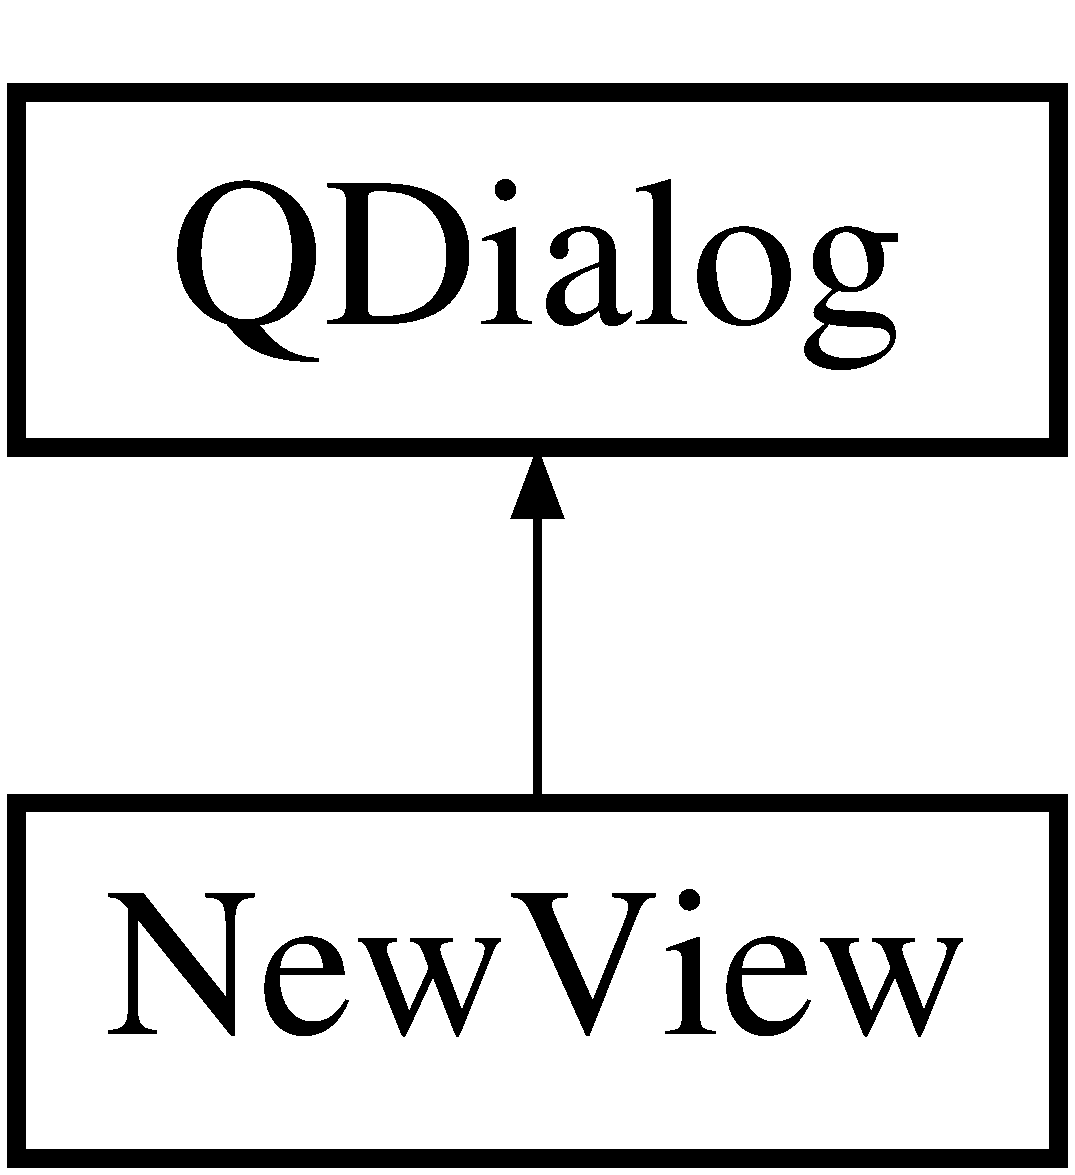
\includegraphics[height=2.000000cm]{classNewView}
\end{center}
\end{figure}
\subsection*{Public Member Functions}
\begin{DoxyCompactItemize}
\item 
\hyperlink{classNewView_adf346776d2dbb084ffd8fae4239d85f3}{New\-View} (Q\-Widget $\ast$parent=0, const Q\-String \&lib\-Name=\char`\"{}\char`\"{}, const Q\-String \&cell\-Name=\char`\"{}\char`\"{})
\begin{DoxyCompactList}\small\item\em Constracts a \hyperlink{classNewView}{New\-View} dialog window to let user select which type of views to create. \end{DoxyCompactList}\item 
\hyperlink{classNewView_ab2bb30c39ce51c8a246dcdeb5c72ef72}{$\sim$\-New\-View} ()
\begin{DoxyCompactList}\small\item\em Destructs \hyperlink{classNewView}{New\-View} obejct and clears up U\-I members. \end{DoxyCompactList}\end{DoxyCompactItemize}
\subsection*{Private Slots}
\begin{DoxyCompactItemize}
\item 
void \hyperlink{classNewView_a1420ad9f114c7a5ff01f55195d7378bd}{on\-\_\-btn\-Cancel\-\_\-clicked} ()
\begin{DoxyCompactList}\small\item\em Closes \hyperlink{classNewView}{New\-View} window. \end{DoxyCompactList}\item 
void \hyperlink{classNewView_a0a34135b4013988f3276bce43782c8ea}{on\-\_\-btn\-Create\-\_\-clicked} ()
\begin{DoxyCompactList}\small\item\em Creates view based on user input and closes the \hyperlink{classNewView}{New\-View} window. \end{DoxyCompactList}\end{DoxyCompactItemize}
\subsection*{Private Member Functions}
\begin{DoxyCompactItemize}
\item 
void \hyperlink{classNewView_aa364531816409ad712b7ea54eba38ee4}{set\-Current\-View\-Type} (const Q\-String \&)
\begin{DoxyCompactList}\small\item\em Sets the provided type name to be the current one in the view type Combo\-Box. \end{DoxyCompactList}\end{DoxyCompactItemize}
\subsection*{Private Attributes}
\begin{DoxyCompactItemize}
\item 
Ui\-::\-New\-View $\ast$ \hyperlink{classNewView_ab8a3d70ca1c0826d69d4411a21f365e0}{m\-\_\-ui}
\item 
\hyperlink{classMainWindow}{Main\-Window} $\ast$ \hyperlink{classNewView_a086dc0337a001800ccd5abaef3f7d815}{m\-\_\-mw}
\end{DoxyCompactItemize}


\subsection{Detailed Description}
The \hyperlink{classNewView}{New\-View} class creates a dialog box where user can select which view to be created. 



 

\subsection{Constructor \& Destructor Documentation}
\hypertarget{classNewView_adf346776d2dbb084ffd8fae4239d85f3}{\index{New\-View@{New\-View}!New\-View@{New\-View}}
\index{New\-View@{New\-View}!NewView@{New\-View}}
\subsubsection[{New\-View}]{\setlength{\rightskip}{0pt plus 5cm}New\-View\-::\-New\-View (
\begin{DoxyParamCaption}
\item[{Q\-Widget $\ast$}]{parent = {\ttfamily 0}, }
\item[{const Q\-String \&}]{lib\-Name = {\ttfamily \char`\"{}\char`\"{}}, }
\item[{const Q\-String \&}]{cell\-Name = {\ttfamily \char`\"{}\char`\"{}}}
\end{DoxyParamCaption}
)\hspace{0.3cm}{\ttfamily [explicit]}}}\label{classNewView_adf346776d2dbb084ffd8fae4239d85f3}


Constracts a \hyperlink{classNewView}{New\-View} dialog window to let user select which type of views to create. 



 
\begin{DoxyParams}{Parameters}
{\em parent} & Parent widget, by default is N\-U\-L\-L. \\
\hline
{\em lib\-Name} & Name of the library. Be default, it is empty. \\
\hline
{\em cell\-Name} & Name of the cell. Be default, it is empty. \\
\hline
\end{DoxyParams}
\hypertarget{classNewView_ab2bb30c39ce51c8a246dcdeb5c72ef72}{\index{New\-View@{New\-View}!$\sim$\-New\-View@{$\sim$\-New\-View}}
\index{$\sim$\-New\-View@{$\sim$\-New\-View}!NewView@{New\-View}}
\subsubsection[{$\sim$\-New\-View}]{\setlength{\rightskip}{0pt plus 5cm}New\-View\-::$\sim$\-New\-View (
\begin{DoxyParamCaption}
{}
\end{DoxyParamCaption}
)}}\label{classNewView_ab2bb30c39ce51c8a246dcdeb5c72ef72}


Destructs \hyperlink{classNewView}{New\-View} obejct and clears up U\-I members. 



 

\subsection{Member Function Documentation}
\hypertarget{classNewView_a1420ad9f114c7a5ff01f55195d7378bd}{\index{New\-View@{New\-View}!on\-\_\-btn\-Cancel\-\_\-clicked@{on\-\_\-btn\-Cancel\-\_\-clicked}}
\index{on\-\_\-btn\-Cancel\-\_\-clicked@{on\-\_\-btn\-Cancel\-\_\-clicked}!NewView@{New\-View}}
\subsubsection[{on\-\_\-btn\-Cancel\-\_\-clicked}]{\setlength{\rightskip}{0pt plus 5cm}void New\-View\-::on\-\_\-btn\-Cancel\-\_\-clicked (
\begin{DoxyParamCaption}
{}
\end{DoxyParamCaption}
)\hspace{0.3cm}{\ttfamily [private]}, {\ttfamily [slot]}}}\label{classNewView_a1420ad9f114c7a5ff01f55195d7378bd}


Closes \hyperlink{classNewView}{New\-View} window. 



 \hypertarget{classNewView_a0a34135b4013988f3276bce43782c8ea}{\index{New\-View@{New\-View}!on\-\_\-btn\-Create\-\_\-clicked@{on\-\_\-btn\-Create\-\_\-clicked}}
\index{on\-\_\-btn\-Create\-\_\-clicked@{on\-\_\-btn\-Create\-\_\-clicked}!NewView@{New\-View}}
\subsubsection[{on\-\_\-btn\-Create\-\_\-clicked}]{\setlength{\rightskip}{0pt plus 5cm}void New\-View\-::on\-\_\-btn\-Create\-\_\-clicked (
\begin{DoxyParamCaption}
{}
\end{DoxyParamCaption}
)\hspace{0.3cm}{\ttfamily [private]}, {\ttfamily [slot]}}}\label{classNewView_a0a34135b4013988f3276bce43782c8ea}


Creates view based on user input and closes the \hyperlink{classNewView}{New\-View} window. 



 \hypertarget{classNewView_aa364531816409ad712b7ea54eba38ee4}{\index{New\-View@{New\-View}!set\-Current\-View\-Type@{set\-Current\-View\-Type}}
\index{set\-Current\-View\-Type@{set\-Current\-View\-Type}!NewView@{New\-View}}
\subsubsection[{set\-Current\-View\-Type}]{\setlength{\rightskip}{0pt plus 5cm}void New\-View\-::set\-Current\-View\-Type (
\begin{DoxyParamCaption}
\item[{const Q\-String \&}]{type}
\end{DoxyParamCaption}
)\hspace{0.3cm}{\ttfamily [private]}}}\label{classNewView_aa364531816409ad712b7ea54eba38ee4}


Sets the provided type name to be the current one in the view type Combo\-Box. 



 
\begin{DoxyParams}{Parameters}
{\em type} & Name of view type (ex., cdl, gds, spice, etc.). \\
\hline
\end{DoxyParams}


\subsection{Member Data Documentation}
\hypertarget{classNewView_a086dc0337a001800ccd5abaef3f7d815}{\index{New\-View@{New\-View}!m\-\_\-mw@{m\-\_\-mw}}
\index{m\-\_\-mw@{m\-\_\-mw}!NewView@{New\-View}}
\subsubsection[{m\-\_\-mw}]{\setlength{\rightskip}{0pt plus 5cm}{\bf Main\-Window}$\ast$ New\-View\-::m\-\_\-mw\hspace{0.3cm}{\ttfamily [private]}}}\label{classNewView_a086dc0337a001800ccd5abaef3f7d815}
A pointer to \hyperlink{classMainWindow}{Main\-Window} object. \hypertarget{classNewView_ab8a3d70ca1c0826d69d4411a21f365e0}{\index{New\-View@{New\-View}!m\-\_\-ui@{m\-\_\-ui}}
\index{m\-\_\-ui@{m\-\_\-ui}!NewView@{New\-View}}
\subsubsection[{m\-\_\-ui}]{\setlength{\rightskip}{0pt plus 5cm}Ui\-::\-New\-View$\ast$ New\-View\-::m\-\_\-ui\hspace{0.3cm}{\ttfamily [private]}}}\label{classNewView_ab8a3d70ca1c0826d69d4411a21f365e0}
A pointer to access \hyperlink{classNewView}{New\-View} graphic items. 

The documentation for this class was generated from the following files\-:\begin{DoxyCompactItemize}
\item 
newview.\-h\item 
newview.\-cpp\end{DoxyCompactItemize}

\hypertarget{classProjectManager}{\section{Project\-Manager Class Reference}
\label{classProjectManager}\index{Project\-Manager@{Project\-Manager}}
}


The \hyperlink{classProjectManager}{Project\-Manager} class creates a dialog window to allow user controlling Lib\-Man projects.  




{\ttfamily \#include $<$projectmanager.\-h$>$}

Inheritance diagram for Project\-Manager\-:\begin{figure}[H]
\begin{center}
\leavevmode
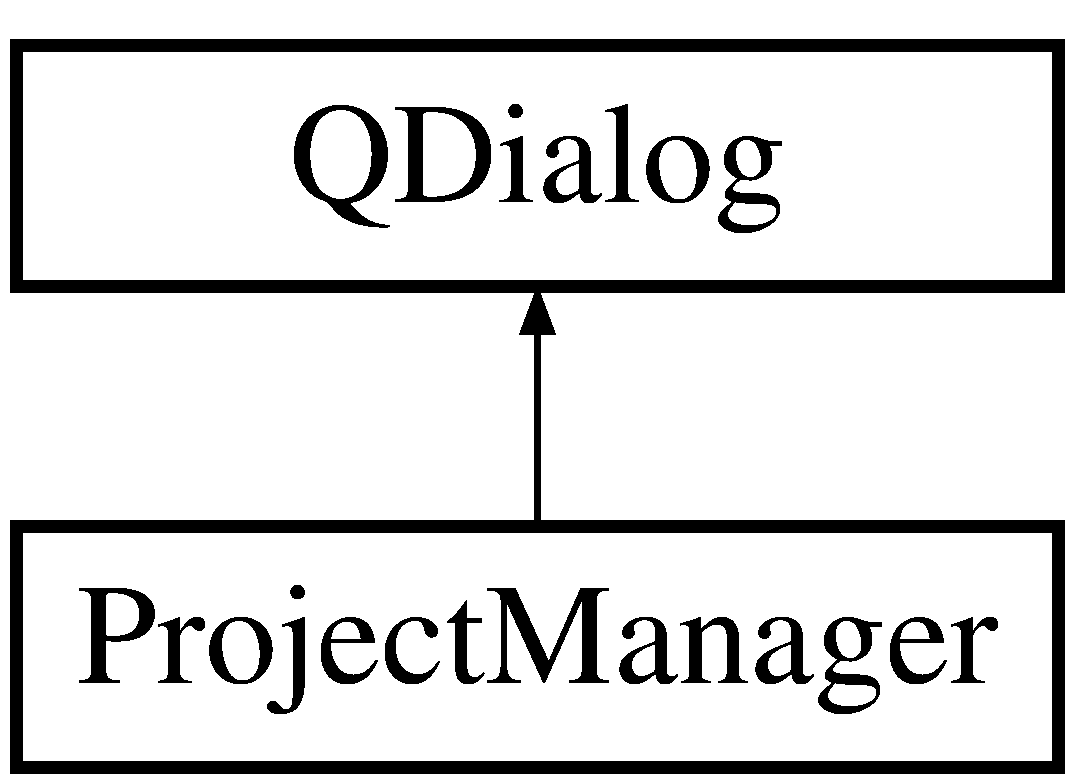
\includegraphics[height=2.000000cm]{classProjectManager}
\end{center}
\end{figure}
\subsection*{Public Member Functions}
\begin{DoxyCompactItemize}
\item 
\hyperlink{classProjectManager_a6a4f1ae5a6cda6ad872aaac00612f9da}{Project\-Manager} (Q\-Widget $\ast$parent, \hyperlink{classProperties}{Properties} $\ast$properties)
\begin{DoxyCompactList}\small\item\em Creates \hyperlink{classToolManager}{Tool\-Manager} object to give user an opportunity to add, rename and remove projects from a dialog window. \end{DoxyCompactList}\item 
\hyperlink{classProjectManager_ac127c8454c7c2caa948ad270930efa86}{$\sim$\-Project\-Manager} ()
\begin{DoxyCompactList}\small\item\em Destructs \hyperlink{classProjectManager}{Project\-Manager} obejct and clears up U\-I members. \end{DoxyCompactList}\end{DoxyCompactItemize}
\subsection*{Private Slots}
\begin{DoxyCompactItemize}
\item 
void \hyperlink{classProjectManager_ad03d75a04852c5f4d85dd5ede30c2a71}{close\-Event} (Q\-Close\-Event $\ast$)
\begin{DoxyCompactList}\small\item\em If state of the \hyperlink{classProjectManager}{Project\-Manager} has been changed the dialog window pops up to ask user for saving of the changes. \end{DoxyCompactList}\item 
void \hyperlink{classProjectManager_ad8697c2b5edaa3aeda168de093139254}{settings\-Changed} (Qt\-Property $\ast$, Q\-Variant)
\begin{DoxyCompactList}\small\item\em The slot is triggered once user changes projects (add, remove, rename). \end{DoxyCompactList}\item 
void \hyperlink{classProjectManager_acbe13c3a4fd77ebbc0437d3c9ecfe78e}{on\-\_\-btn\-Ok\-\_\-clicked} ()
\begin{DoxyCompactList}\small\item\em Saves current tool projects into properties of \hyperlink{classMainWindow}{Main\-Window} object and closes the window. \end{DoxyCompactList}\item 
void \hyperlink{classProjectManager_a808da17a51773b55f6330f7c11cbdbef}{on\-\_\-btn\-Cancel\-\_\-clicked} ()
\begin{DoxyCompactList}\small\item\em closes \hyperlink{classProjectManager}{Project\-Manager} window. \end{DoxyCompactList}\end{DoxyCompactItemize}
\subsection*{Private Member Functions}
\begin{DoxyCompactItemize}
\item 
void \hyperlink{classProjectManager_afdb622867c005d726057a288fcf56d33}{init} ()
\begin{DoxyCompactList}\small\item\em Initializes Qt\-Tree\-Property\-Browser and creates its properties. It's used to manage a list of projects that can be chosen by user for further work. \end{DoxyCompactList}\item 
\hypertarget{classProjectManager_ad397c063f9164728884beaf221ce03b0}{bool {\bfseries is\-State\-Changed} () const }\label{classProjectManager_ad397c063f9164728884beaf221ce03b0}

\item 
void \hyperlink{classProjectManager_a89c55c9616362e13ef4fd81de2a2389b}{set\-State\-Saved} ()
\begin{DoxyCompactList}\small\item\em Set state of \hyperlink{classProjectManager}{Project\-Manager} dialog window saved (unchanged). \end{DoxyCompactList}\item 
void \hyperlink{classProjectManager_ac178fe4a0ff88ce4b860fa92373f6e23}{set\-State\-Changed} ()
\begin{DoxyCompactList}\small\item\em Sets the state chaged if project(s) has(have) been modified. \end{DoxyCompactList}\end{DoxyCompactItemize}
\subsection*{Private Attributes}
\begin{DoxyCompactItemize}
\item 
Ui\-::\-Project\-Manager $\ast$ \hyperlink{classProjectManager_a522b0621f0ca1978d0cef23fc553fd5e}{m\-\_\-ui}
\item 
\hyperlink{classMainWindow}{Main\-Window} $\ast$ \hyperlink{classProjectManager_a854e94a40ac35e0dc3fe45ef12ff855a}{m\-\_\-mw}
\item 
bool \hyperlink{classProjectManager_aa7cad9fe90b6a9bbaa0ae6d727d12e7c}{m\-\_\-is\-State\-Changed}
\item 
\hyperlink{classProperties}{Properties} $\ast$ \hyperlink{classProjectManager_afa1e791a680f491f89aa215a5198f06a}{m\-\_\-properties}
\item 
Qt\-Tree\-Property\-Browser $\ast$ \hyperlink{classProjectManager_a9c23c2284358dd111bc1b29f6ca6f611}{m\-\_\-pb\-Settings}
\item 
Qt\-Variant\-Property\-Manager $\ast$ \hyperlink{classProjectManager_a713a455e7c92cc5875d590c6d4bb0bf0}{m\-\_\-vm\-Settings}
\end{DoxyCompactItemize}


\subsection{Detailed Description}
The \hyperlink{classProjectManager}{Project\-Manager} class creates a dialog window to allow user controlling Lib\-Man projects. 



 

\subsection{Constructor \& Destructor Documentation}
\hypertarget{classProjectManager_a6a4f1ae5a6cda6ad872aaac00612f9da}{\index{Project\-Manager@{Project\-Manager}!Project\-Manager@{Project\-Manager}}
\index{Project\-Manager@{Project\-Manager}!ProjectManager@{Project\-Manager}}
\subsubsection[{Project\-Manager}]{\setlength{\rightskip}{0pt plus 5cm}Project\-Manager\-::\-Project\-Manager (
\begin{DoxyParamCaption}
\item[{Q\-Widget $\ast$}]{parent, }
\item[{{\bf Properties} $\ast$}]{properties}
\end{DoxyParamCaption}
)\hspace{0.3cm}{\ttfamily [explicit]}}}\label{classProjectManager_a6a4f1ae5a6cda6ad872aaac00612f9da}


Creates \hyperlink{classToolManager}{Tool\-Manager} object to give user an opportunity to add, rename and remove projects from a dialog window. 



 
\begin{DoxyParams}{Parameters}
{\em parent} & Parent widget, by default is N\-U\-L\-L. \\
\hline
{\em properties} & Container of Lib\-Man settings. \\
\hline
\end{DoxyParams}
\hypertarget{classProjectManager_ac127c8454c7c2caa948ad270930efa86}{\index{Project\-Manager@{Project\-Manager}!$\sim$\-Project\-Manager@{$\sim$\-Project\-Manager}}
\index{$\sim$\-Project\-Manager@{$\sim$\-Project\-Manager}!ProjectManager@{Project\-Manager}}
\subsubsection[{$\sim$\-Project\-Manager}]{\setlength{\rightskip}{0pt plus 5cm}Project\-Manager\-::$\sim$\-Project\-Manager (
\begin{DoxyParamCaption}
{}
\end{DoxyParamCaption}
)}}\label{classProjectManager_ac127c8454c7c2caa948ad270930efa86}


Destructs \hyperlink{classProjectManager}{Project\-Manager} obejct and clears up U\-I members. 



 

\subsection{Member Function Documentation}
\hypertarget{classProjectManager_ad03d75a04852c5f4d85dd5ede30c2a71}{\index{Project\-Manager@{Project\-Manager}!close\-Event@{close\-Event}}
\index{close\-Event@{close\-Event}!ProjectManager@{Project\-Manager}}
\subsubsection[{close\-Event}]{\setlength{\rightskip}{0pt plus 5cm}void Project\-Manager\-::close\-Event (
\begin{DoxyParamCaption}
\item[{Q\-Close\-Event $\ast$}]{event}
\end{DoxyParamCaption}
)\hspace{0.3cm}{\ttfamily [private]}, {\ttfamily [slot]}}}\label{classProjectManager_ad03d75a04852c5f4d85dd5ede30c2a71}


If state of the \hyperlink{classProjectManager}{Project\-Manager} has been changed the dialog window pops up to ask user for saving of the changes. 



 
\begin{DoxyParams}{Parameters}
{\em event} & Variable is used to either accept to close the window or ignore to prevent closing it. \\
\hline
\end{DoxyParams}
\hypertarget{classProjectManager_afdb622867c005d726057a288fcf56d33}{\index{Project\-Manager@{Project\-Manager}!init@{init}}
\index{init@{init}!ProjectManager@{Project\-Manager}}
\subsubsection[{init}]{\setlength{\rightskip}{0pt plus 5cm}void Project\-Manager\-::init (
\begin{DoxyParamCaption}
{}
\end{DoxyParamCaption}
)\hspace{0.3cm}{\ttfamily [private]}}}\label{classProjectManager_afdb622867c005d726057a288fcf56d33}


Initializes Qt\-Tree\-Property\-Browser and creates its properties. It's used to manage a list of projects that can be chosen by user for further work. 



 \hypertarget{classProjectManager_a808da17a51773b55f6330f7c11cbdbef}{\index{Project\-Manager@{Project\-Manager}!on\-\_\-btn\-Cancel\-\_\-clicked@{on\-\_\-btn\-Cancel\-\_\-clicked}}
\index{on\-\_\-btn\-Cancel\-\_\-clicked@{on\-\_\-btn\-Cancel\-\_\-clicked}!ProjectManager@{Project\-Manager}}
\subsubsection[{on\-\_\-btn\-Cancel\-\_\-clicked}]{\setlength{\rightskip}{0pt plus 5cm}void Project\-Manager\-::on\-\_\-btn\-Cancel\-\_\-clicked (
\begin{DoxyParamCaption}
{}
\end{DoxyParamCaption}
)\hspace{0.3cm}{\ttfamily [private]}, {\ttfamily [slot]}}}\label{classProjectManager_a808da17a51773b55f6330f7c11cbdbef}


closes \hyperlink{classProjectManager}{Project\-Manager} window. 



 \hypertarget{classProjectManager_acbe13c3a4fd77ebbc0437d3c9ecfe78e}{\index{Project\-Manager@{Project\-Manager}!on\-\_\-btn\-Ok\-\_\-clicked@{on\-\_\-btn\-Ok\-\_\-clicked}}
\index{on\-\_\-btn\-Ok\-\_\-clicked@{on\-\_\-btn\-Ok\-\_\-clicked}!ProjectManager@{Project\-Manager}}
\subsubsection[{on\-\_\-btn\-Ok\-\_\-clicked}]{\setlength{\rightskip}{0pt plus 5cm}void Project\-Manager\-::on\-\_\-btn\-Ok\-\_\-clicked (
\begin{DoxyParamCaption}
{}
\end{DoxyParamCaption}
)\hspace{0.3cm}{\ttfamily [private]}, {\ttfamily [slot]}}}\label{classProjectManager_acbe13c3a4fd77ebbc0437d3c9ecfe78e}


Saves current tool projects into properties of \hyperlink{classMainWindow}{Main\-Window} object and closes the window. 



 \hypertarget{classProjectManager_ac178fe4a0ff88ce4b860fa92373f6e23}{\index{Project\-Manager@{Project\-Manager}!set\-State\-Changed@{set\-State\-Changed}}
\index{set\-State\-Changed@{set\-State\-Changed}!ProjectManager@{Project\-Manager}}
\subsubsection[{set\-State\-Changed}]{\setlength{\rightskip}{0pt plus 5cm}void Project\-Manager\-::set\-State\-Changed (
\begin{DoxyParamCaption}
{}
\end{DoxyParamCaption}
)\hspace{0.3cm}{\ttfamily [private]}}}\label{classProjectManager_ac178fe4a0ff88ce4b860fa92373f6e23}


Sets the state chaged if project(s) has(have) been modified. 



 \hypertarget{classProjectManager_a89c55c9616362e13ef4fd81de2a2389b}{\index{Project\-Manager@{Project\-Manager}!set\-State\-Saved@{set\-State\-Saved}}
\index{set\-State\-Saved@{set\-State\-Saved}!ProjectManager@{Project\-Manager}}
\subsubsection[{set\-State\-Saved}]{\setlength{\rightskip}{0pt plus 5cm}void Project\-Manager\-::set\-State\-Saved (
\begin{DoxyParamCaption}
{}
\end{DoxyParamCaption}
)\hspace{0.3cm}{\ttfamily [private]}}}\label{classProjectManager_a89c55c9616362e13ef4fd81de2a2389b}


Set state of \hyperlink{classProjectManager}{Project\-Manager} dialog window saved (unchanged). 



 \hypertarget{classProjectManager_ad8697c2b5edaa3aeda168de093139254}{\index{Project\-Manager@{Project\-Manager}!settings\-Changed@{settings\-Changed}}
\index{settings\-Changed@{settings\-Changed}!ProjectManager@{Project\-Manager}}
\subsubsection[{settings\-Changed}]{\setlength{\rightskip}{0pt plus 5cm}void Project\-Manager\-::settings\-Changed (
\begin{DoxyParamCaption}
\item[{Qt\-Property $\ast$}]{, }
\item[{Q\-Variant}]{}
\end{DoxyParamCaption}
)\hspace{0.3cm}{\ttfamily [private]}, {\ttfamily [slot]}}}\label{classProjectManager_ad8697c2b5edaa3aeda168de093139254}


The slot is triggered once user changes projects (add, remove, rename). 



 

\subsection{Member Data Documentation}
\hypertarget{classProjectManager_aa7cad9fe90b6a9bbaa0ae6d727d12e7c}{\index{Project\-Manager@{Project\-Manager}!m\-\_\-is\-State\-Changed@{m\-\_\-is\-State\-Changed}}
\index{m\-\_\-is\-State\-Changed@{m\-\_\-is\-State\-Changed}!ProjectManager@{Project\-Manager}}
\subsubsection[{m\-\_\-is\-State\-Changed}]{\setlength{\rightskip}{0pt plus 5cm}bool Project\-Manager\-::m\-\_\-is\-State\-Changed\hspace{0.3cm}{\ttfamily [private]}}}\label{classProjectManager_aa7cad9fe90b6a9bbaa0ae6d727d12e7c}
Keeps the state of the \hyperlink{classProjectManager}{Project\-Manager} dialog window session. \hypertarget{classProjectManager_a854e94a40ac35e0dc3fe45ef12ff855a}{\index{Project\-Manager@{Project\-Manager}!m\-\_\-mw@{m\-\_\-mw}}
\index{m\-\_\-mw@{m\-\_\-mw}!ProjectManager@{Project\-Manager}}
\subsubsection[{m\-\_\-mw}]{\setlength{\rightskip}{0pt plus 5cm}{\bf Main\-Window}$\ast$ Project\-Manager\-::m\-\_\-mw\hspace{0.3cm}{\ttfamily [private]}}}\label{classProjectManager_a854e94a40ac35e0dc3fe45ef12ff855a}
A pointer to acess \hyperlink{classMainWindow}{Main\-Window} items as it's a friend class. \hypertarget{classProjectManager_a9c23c2284358dd111bc1b29f6ca6f611}{\index{Project\-Manager@{Project\-Manager}!m\-\_\-pb\-Settings@{m\-\_\-pb\-Settings}}
\index{m\-\_\-pb\-Settings@{m\-\_\-pb\-Settings}!ProjectManager@{Project\-Manager}}
\subsubsection[{m\-\_\-pb\-Settings}]{\setlength{\rightskip}{0pt plus 5cm}Qt\-Tree\-Property\-Browser$\ast$ Project\-Manager\-::m\-\_\-pb\-Settings\hspace{0.3cm}{\ttfamily [private]}}}\label{classProjectManager_a9c23c2284358dd111bc1b29f6ca6f611}
A property browser framework enabling the user to edit a set of properties. \hypertarget{classProjectManager_afa1e791a680f491f89aa215a5198f06a}{\index{Project\-Manager@{Project\-Manager}!m\-\_\-properties@{m\-\_\-properties}}
\index{m\-\_\-properties@{m\-\_\-properties}!ProjectManager@{Project\-Manager}}
\subsubsection[{m\-\_\-properties}]{\setlength{\rightskip}{0pt plus 5cm}{\bf Properties}$\ast$ Project\-Manager\-::m\-\_\-properties\hspace{0.3cm}{\ttfamily [private]}}}\label{classProjectManager_afa1e791a680f491f89aa215a5198f06a}
Container to store Lib\-Man settings. \hypertarget{classProjectManager_a522b0621f0ca1978d0cef23fc553fd5e}{\index{Project\-Manager@{Project\-Manager}!m\-\_\-ui@{m\-\_\-ui}}
\index{m\-\_\-ui@{m\-\_\-ui}!ProjectManager@{Project\-Manager}}
\subsubsection[{m\-\_\-ui}]{\setlength{\rightskip}{0pt plus 5cm}Ui\-::\-Project\-Manager$\ast$ Project\-Manager\-::m\-\_\-ui\hspace{0.3cm}{\ttfamily [private]}}}\label{classProjectManager_a522b0621f0ca1978d0cef23fc553fd5e}
A pointer to acess \hyperlink{classProjectManager}{Project\-Manager} graphic items. \hypertarget{classProjectManager_a713a455e7c92cc5875d590c6d4bb0bf0}{\index{Project\-Manager@{Project\-Manager}!m\-\_\-vm\-Settings@{m\-\_\-vm\-Settings}}
\index{m\-\_\-vm\-Settings@{m\-\_\-vm\-Settings}!ProjectManager@{Project\-Manager}}
\subsubsection[{m\-\_\-vm\-Settings}]{\setlength{\rightskip}{0pt plus 5cm}Qt\-Variant\-Property\-Manager$\ast$ Project\-Manager\-::m\-\_\-vm\-Settings\hspace{0.3cm}{\ttfamily [private]}}}\label{classProjectManager_a713a455e7c92cc5875d590c6d4bb0bf0}
Each property type, the framework provides a property manager associated with editor factory. 

The documentation for this class was generated from the following files\-:\begin{DoxyCompactItemize}
\item 
projectmanager.\-h\item 
projectmanager.\-cpp\end{DoxyCompactItemize}

\hypertarget{classProperties}{\section{Properties Class Reference}
\label{classProperties}\index{Properties@{Properties}}
}


The \hyperlink{classProperties}{Properties} class stores and manipulates all kind of data types. It is used for managing Lib\-Man settings.  




{\ttfamily \#include $<$property.\-h$>$}

\subsection*{Public Member Functions}
\begin{DoxyCompactItemize}
\item 
\hyperlink{classProperties_a7c001f15168b6ec386377dc91e288033}{Properties} ()
\begin{DoxyCompactList}\small\item\em Constructs \hyperlink{classProperties}{Properties} object. \end{DoxyCompactList}\item 
\hyperlink{classProperties_a9a4367c64d90a962fc260128587670dd}{$\sim$\-Properties} ()
\begin{DoxyCompactList}\small\item\em Destructs \hyperlink{classProperties}{Properties} obejct and clears up the property items. \end{DoxyCompactList}\item 
unsigned \hyperlink{classProperties_af65e2e755382f74208fc9d3411eb7d93}{count} () const 
\begin{DoxyCompactList}\small\item\em Returns number of stored properties. \end{DoxyCompactList}\item 
unsigned \hyperlink{classProperties_a02eae31d56c3ce060acf269808c1aae4}{get\-Value\-Count} (const Q\-String \&name) const 
\begin{DoxyCompactList}\small\item\em Removes property item by name. \end{DoxyCompactList}\item 
void \hyperlink{classProperties_a648567d171b2bac9cdfa8de6fe53a865}{remove} (const Q\-String \&name)
\begin{DoxyCompactList}\small\item\em Removes property item by name. \end{DoxyCompactList}\item 
bool \hyperlink{classProperties_affd1124bf0ea0712a110e99204b55ea2}{exists} (const Q\-String \&name) const 
\begin{DoxyCompactList}\small\item\em Checks if property item is part of the collection. \end{DoxyCompactList}\item 
bool \hyperlink{classProperties_a8dec2d75af8e2871a089eb49c24227c6}{is\-Modified} (const Q\-String \&name) const 
\begin{DoxyCompactList}\small\item\em Cehcks if item has been modified. \end{DoxyCompactList}\item 
Q\-Variant \hyperlink{classProperties_ac987644f72837c216e73c67dbe931e2b}{get\-Variant} (const Q\-String \&name) const 
\begin{DoxyCompactList}\small\item\em Returns propery variant's value. \end{DoxyCompactList}\item 
{\footnotesize template$<$class T $>$ }\\T \hyperlink{classProperties_a4821665cdb6ab25eb9ce4a4681ba0f3c}{get} (const Q\-String \&name) const 
\begin{DoxyCompactList}\small\item\em Returns property item by name. \end{DoxyCompactList}\item 
{\footnotesize template$<$class T $>$ }\\Q\-List$<$ T $>$ \hyperlink{classProperties_a6bc91c0049e2b7b5f87220ad34186eaa}{get\-List} (const Q\-String \&name) const 
\begin{DoxyCompactList}\small\item\em Return list of the property items by property name. \end{DoxyCompactList}\item 
{\footnotesize template$<$class T $>$ }\\void \hyperlink{classProperties_add6b87d7b0d66ef5dd0a9b2d419cae7f}{set} (const Q\-String \&name, const T \&value)
\begin{DoxyCompactList}\small\item\em Assigns a new value to property item. \end{DoxyCompactList}\item 
{\footnotesize template$<$class T $>$ }\\void \hyperlink{classProperties_a695bdfbe49a5a8301dd960076a5ab375}{add} (const Q\-String \&name, const T \&value)
\begin{DoxyCompactList}\small\item\em Adds property value to collection. \end{DoxyCompactList}\item 
{\footnotesize template$<$class T $>$ }\\void \hyperlink{classProperties_a59c39bab253ac2c960a63b811736bad2}{set\-Default} (const Q\-String \&name, const T \&value)
\begin{DoxyCompactList}\small\item\em Sets the default value of property item. \end{DoxyCompactList}\item 
const Q\-Map$<$ Q\-String, \\*
\hyperlink{classPropertyItem}{Property\-Item} $\ast$ $>$ \hyperlink{classProperties_aca02c11425e9c2fb0b76b3f2a7b54b30}{get\-Map} () const 
\begin{DoxyCompactList}\small\item\em Returns collection's map of property items. \end{DoxyCompactList}\end{DoxyCompactItemize}
\subsection*{Private Attributes}
\begin{DoxyCompactItemize}
\item 
\hypertarget{classProperties_afe7bbb30e511d652af272b08c78bf8a9}{Q\-Map$<$ Q\-String, \hyperlink{classPropertyItem}{Property\-Item} $\ast$ $>$ {\bfseries m\-\_\-data}}\label{classProperties_afe7bbb30e511d652af272b08c78bf8a9}

\end{DoxyCompactItemize}


\subsection{Detailed Description}
The \hyperlink{classProperties}{Properties} class stores and manipulates all kind of data types. It is used for managing Lib\-Man settings. 



 

\subsection{Constructor \& Destructor Documentation}
\hypertarget{classProperties_a7c001f15168b6ec386377dc91e288033}{\index{Properties@{Properties}!Properties@{Properties}}
\index{Properties@{Properties}!Properties@{Properties}}
\subsubsection[{Properties}]{\setlength{\rightskip}{0pt plus 5cm}Properties\-::\-Properties (
\begin{DoxyParamCaption}
{}
\end{DoxyParamCaption}
)}}\label{classProperties_a7c001f15168b6ec386377dc91e288033}


Constructs \hyperlink{classProperties}{Properties} object. 



 \hypertarget{classProperties_a9a4367c64d90a962fc260128587670dd}{\index{Properties@{Properties}!$\sim$\-Properties@{$\sim$\-Properties}}
\index{$\sim$\-Properties@{$\sim$\-Properties}!Properties@{Properties}}
\subsubsection[{$\sim$\-Properties}]{\setlength{\rightskip}{0pt plus 5cm}Properties\-::$\sim$\-Properties (
\begin{DoxyParamCaption}
{}
\end{DoxyParamCaption}
)}}\label{classProperties_a9a4367c64d90a962fc260128587670dd}


Destructs \hyperlink{classProperties}{Properties} obejct and clears up the property items. 



 

\subsection{Member Function Documentation}
\hypertarget{classProperties_a695bdfbe49a5a8301dd960076a5ab375}{\index{Properties@{Properties}!add@{add}}
\index{add@{add}!Properties@{Properties}}
\subsubsection[{add}]{\setlength{\rightskip}{0pt plus 5cm}template$<$class T $>$ void Properties\-::add (
\begin{DoxyParamCaption}
\item[{const Q\-String \&}]{name, }
\item[{const T \&}]{value}
\end{DoxyParamCaption}
)\hspace{0.3cm}{\ttfamily [inline]}}}\label{classProperties_a695bdfbe49a5a8301dd960076a5ab375}


Adds property value to collection. 



 
\begin{DoxyParams}{Parameters}
{\em name} & Name of the property item. \\
\hline
{\em value} & Value of the property item. Property can be any of allowed type. \\
\hline
\end{DoxyParams}
\hypertarget{classProperties_af65e2e755382f74208fc9d3411eb7d93}{\index{Properties@{Properties}!count@{count}}
\index{count@{count}!Properties@{Properties}}
\subsubsection[{count}]{\setlength{\rightskip}{0pt plus 5cm}unsigned Properties\-::count (
\begin{DoxyParamCaption}
{}
\end{DoxyParamCaption}
) const\hspace{0.3cm}{\ttfamily [inline]}}}\label{classProperties_af65e2e755382f74208fc9d3411eb7d93}


Returns number of stored properties. 



 \hypertarget{classProperties_affd1124bf0ea0712a110e99204b55ea2}{\index{Properties@{Properties}!exists@{exists}}
\index{exists@{exists}!Properties@{Properties}}
\subsubsection[{exists}]{\setlength{\rightskip}{0pt plus 5cm}bool Properties\-::exists (
\begin{DoxyParamCaption}
\item[{const Q\-String \&}]{name}
\end{DoxyParamCaption}
) const}}\label{classProperties_affd1124bf0ea0712a110e99204b55ea2}


Checks if property item is part of the collection. 



 
\begin{DoxyParams}{Parameters}
{\em name} & Name of the property item. \\
\hline
\end{DoxyParams}
\hypertarget{classProperties_a4821665cdb6ab25eb9ce4a4681ba0f3c}{\index{Properties@{Properties}!get@{get}}
\index{get@{get}!Properties@{Properties}}
\subsubsection[{get}]{\setlength{\rightskip}{0pt plus 5cm}template$<$class T $>$ T Properties\-::get (
\begin{DoxyParamCaption}
\item[{const Q\-String \&}]{name}
\end{DoxyParamCaption}
) const\hspace{0.3cm}{\ttfamily [inline]}}}\label{classProperties_a4821665cdb6ab25eb9ce4a4681ba0f3c}


Returns property item by name. 



 
\begin{DoxyParams}{Parameters}
{\em name} & Name of the property item. \\
\hline
\end{DoxyParams}
\hypertarget{classProperties_a6bc91c0049e2b7b5f87220ad34186eaa}{\index{Properties@{Properties}!get\-List@{get\-List}}
\index{get\-List@{get\-List}!Properties@{Properties}}
\subsubsection[{get\-List}]{\setlength{\rightskip}{0pt plus 5cm}template$<$class T $>$ Q\-List$<$ T $>$ Properties\-::get\-List (
\begin{DoxyParamCaption}
\item[{const Q\-String \&}]{name}
\end{DoxyParamCaption}
) const\hspace{0.3cm}{\ttfamily [inline]}}}\label{classProperties_a6bc91c0049e2b7b5f87220ad34186eaa}


Return list of the property items by property name. 



 
\begin{DoxyParams}{Parameters}
{\em name} & Name of the property item. \\
\hline
\end{DoxyParams}
\hypertarget{classProperties_aca02c11425e9c2fb0b76b3f2a7b54b30}{\index{Properties@{Properties}!get\-Map@{get\-Map}}
\index{get\-Map@{get\-Map}!Properties@{Properties}}
\subsubsection[{get\-Map}]{\setlength{\rightskip}{0pt plus 5cm}const Q\-Map$<$ Q\-String, {\bf Property\-Item} $\ast$ $>$ Properties\-::get\-Map (
\begin{DoxyParamCaption}
{}
\end{DoxyParamCaption}
) const\hspace{0.3cm}{\ttfamily [inline]}}}\label{classProperties_aca02c11425e9c2fb0b76b3f2a7b54b30}


Returns collection's map of property items. 



 \hypertarget{classProperties_a02eae31d56c3ce060acf269808c1aae4}{\index{Properties@{Properties}!get\-Value\-Count@{get\-Value\-Count}}
\index{get\-Value\-Count@{get\-Value\-Count}!Properties@{Properties}}
\subsubsection[{get\-Value\-Count}]{\setlength{\rightskip}{0pt plus 5cm}unsigned Properties\-::get\-Value\-Count (
\begin{DoxyParamCaption}
\item[{const Q\-String \&}]{name}
\end{DoxyParamCaption}
) const\hspace{0.3cm}{\ttfamily [inline]}}}\label{classProperties_a02eae31d56c3ce060acf269808c1aae4}


Removes property item by name. 



 
\begin{DoxyParams}{Parameters}
{\em name} & Name of the property item to be removed. \\
\hline
\end{DoxyParams}
\hypertarget{classProperties_ac987644f72837c216e73c67dbe931e2b}{\index{Properties@{Properties}!get\-Variant@{get\-Variant}}
\index{get\-Variant@{get\-Variant}!Properties@{Properties}}
\subsubsection[{get\-Variant}]{\setlength{\rightskip}{0pt plus 5cm}Q\-Variant Properties\-::get\-Variant (
\begin{DoxyParamCaption}
\item[{const Q\-String \&}]{name}
\end{DoxyParamCaption}
) const}}\label{classProperties_ac987644f72837c216e73c67dbe931e2b}


Returns propery variant's value. 



 
\begin{DoxyParams}{Parameters}
{\em name} & Name of the property item. \\
\hline
\end{DoxyParams}
\hypertarget{classProperties_a8dec2d75af8e2871a089eb49c24227c6}{\index{Properties@{Properties}!is\-Modified@{is\-Modified}}
\index{is\-Modified@{is\-Modified}!Properties@{Properties}}
\subsubsection[{is\-Modified}]{\setlength{\rightskip}{0pt plus 5cm}bool Properties\-::is\-Modified (
\begin{DoxyParamCaption}
\item[{const Q\-String \&}]{name}
\end{DoxyParamCaption}
) const}}\label{classProperties_a8dec2d75af8e2871a089eb49c24227c6}


Cehcks if item has been modified. 



 
\begin{DoxyParams}{Parameters}
{\em name} & Name of the property item. \\
\hline
\end{DoxyParams}
\hypertarget{classProperties_a648567d171b2bac9cdfa8de6fe53a865}{\index{Properties@{Properties}!remove@{remove}}
\index{remove@{remove}!Properties@{Properties}}
\subsubsection[{remove}]{\setlength{\rightskip}{0pt plus 5cm}void Properties\-::remove (
\begin{DoxyParamCaption}
\item[{const Q\-String \&}]{name}
\end{DoxyParamCaption}
)\hspace{0.3cm}{\ttfamily [inline]}}}\label{classProperties_a648567d171b2bac9cdfa8de6fe53a865}


Removes property item by name. 



 
\begin{DoxyParams}{Parameters}
{\em name} & Name of the property to be removed. \\
\hline
\end{DoxyParams}
\hypertarget{classProperties_add6b87d7b0d66ef5dd0a9b2d419cae7f}{\index{Properties@{Properties}!set@{set}}
\index{set@{set}!Properties@{Properties}}
\subsubsection[{set}]{\setlength{\rightskip}{0pt plus 5cm}template$<$class T $>$ void Properties\-::set (
\begin{DoxyParamCaption}
\item[{const Q\-String \&}]{name, }
\item[{const T \&}]{value}
\end{DoxyParamCaption}
)\hspace{0.3cm}{\ttfamily [inline]}}}\label{classProperties_add6b87d7b0d66ef5dd0a9b2d419cae7f}


Assigns a new value to property item. 



 
\begin{DoxyParams}{Parameters}
{\em name} & Name of the property item. \\
\hline
{\em name} & Value of the property item. Property can be any of allowed type. \\
\hline
\end{DoxyParams}
\hypertarget{classProperties_a59c39bab253ac2c960a63b811736bad2}{\index{Properties@{Properties}!set\-Default@{set\-Default}}
\index{set\-Default@{set\-Default}!Properties@{Properties}}
\subsubsection[{set\-Default}]{\setlength{\rightskip}{0pt plus 5cm}template$<$class T $>$ void Properties\-::set\-Default (
\begin{DoxyParamCaption}
\item[{const Q\-String \&}]{name, }
\item[{const T \&}]{value}
\end{DoxyParamCaption}
)\hspace{0.3cm}{\ttfamily [inline]}}}\label{classProperties_a59c39bab253ac2c960a63b811736bad2}


Sets the default value of property item. 



 
\begin{DoxyParams}{Parameters}
{\em name} & Name of the property item. \\
\hline
{\em value} & Value of the property item. Property can be any of allowed type. \\
\hline
\end{DoxyParams}


The documentation for this class was generated from the following files\-:\begin{DoxyCompactItemize}
\item 
property.\-h\item 
property.\-cpp\end{DoxyCompactItemize}

\hypertarget{classPropertyItem}{\section{Property\-Item Class Reference}
\label{classPropertyItem}\index{Property\-Item@{Property\-Item}}
}


The \hyperlink{classPropertyItem}{Property\-Item} class creates a single object of any type used by the \hyperlink{classProperties}{Properties} class.  




{\ttfamily \#include $<$property.\-h$>$}

\subsection*{Public Member Functions}
\begin{DoxyCompactItemize}
\item 
\hyperlink{classPropertyItem_aba8c67d9932b6cebec39d46853e9c5e0}{Property\-Item} (const Q\-Variant, bool modyfied=false)
\begin{DoxyCompactList}\small\item\em Constructs \hyperlink{classPropertyItem}{Property\-Item} object. \end{DoxyCompactList}\item 
\hyperlink{classPropertyItem_a0359155d78184d85b2e0360490b2ffe0}{$\sim$\-Property\-Item} ()
\begin{DoxyCompactList}\small\item\em Destructs \hyperlink{classPropertyItem}{Property\-Item} obejct and clears up the property items values. \end{DoxyCompactList}\item 
Q\-List$<$ Q\-Variant $>$ \hyperlink{classPropertyItem_a02d785cac9092258b7899f9a3a6f1bdd}{get\-Value} () const 
\begin{DoxyCompactList}\small\item\em Returns item's property value. \end{DoxyCompactList}\item 
bool \hyperlink{classPropertyItem_aac35d432deca70783d3e45ab26d06e33}{is\-Modified} () const 
\begin{DoxyCompactList}\small\item\em Returns the state if property has been modified or not. \end{DoxyCompactList}\item 
void \hyperlink{classPropertyItem_aaf7e9ff216f4136ed04be644f6755a82}{add\-Value} (const Q\-Variant)
\begin{DoxyCompactList}\small\item\em \hyperlink{classPropertyItem_aaf7e9ff216f4136ed04be644f6755a82}{Property\-Item\-::add\-Value}. \end{DoxyCompactList}\end{DoxyCompactItemize}
\subsection*{Private Attributes}
\begin{DoxyCompactItemize}
\item 
Q\-List$<$ Q\-Variant $>$ \hyperlink{classPropertyItem_aa9c03a1e9828de471e73df1d30e4abdb}{m\-\_\-value}
\item 
bool \hyperlink{classPropertyItem_a464bcb9ada09b86548daa191c9225ead}{m\-\_\-status}
\end{DoxyCompactItemize}


\subsection{Detailed Description}
The \hyperlink{classPropertyItem}{Property\-Item} class creates a single object of any type used by the \hyperlink{classProperties}{Properties} class. 



 

\subsection{Constructor \& Destructor Documentation}
\hypertarget{classPropertyItem_aba8c67d9932b6cebec39d46853e9c5e0}{\index{Property\-Item@{Property\-Item}!Property\-Item@{Property\-Item}}
\index{Property\-Item@{Property\-Item}!PropertyItem@{Property\-Item}}
\subsubsection[{Property\-Item}]{\setlength{\rightskip}{0pt plus 5cm}Property\-Item\-::\-Property\-Item (
\begin{DoxyParamCaption}
\item[{const Q\-Variant}]{value, }
\item[{bool}]{modyfied = {\ttfamily false}}
\end{DoxyParamCaption}
)}}\label{classPropertyItem_aba8c67d9932b6cebec39d46853e9c5e0}


Constructs \hyperlink{classPropertyItem}{Property\-Item} object. 



 
\begin{DoxyParams}{Parameters}
{\em value} & Name of the property item. \\
\hline
{\em modyfied} & Flag value if item has been modified. Allows setting it to false by adding new value. \\
\hline
\end{DoxyParams}
\hypertarget{classPropertyItem_a0359155d78184d85b2e0360490b2ffe0}{\index{Property\-Item@{Property\-Item}!$\sim$\-Property\-Item@{$\sim$\-Property\-Item}}
\index{$\sim$\-Property\-Item@{$\sim$\-Property\-Item}!PropertyItem@{Property\-Item}}
\subsubsection[{$\sim$\-Property\-Item}]{\setlength{\rightskip}{0pt plus 5cm}Property\-Item\-::$\sim$\-Property\-Item (
\begin{DoxyParamCaption}
{}
\end{DoxyParamCaption}
)}}\label{classPropertyItem_a0359155d78184d85b2e0360490b2ffe0}


Destructs \hyperlink{classPropertyItem}{Property\-Item} obejct and clears up the property items values. 



 

\subsection{Member Function Documentation}
\hypertarget{classPropertyItem_aaf7e9ff216f4136ed04be644f6755a82}{\index{Property\-Item@{Property\-Item}!add\-Value@{add\-Value}}
\index{add\-Value@{add\-Value}!PropertyItem@{Property\-Item}}
\subsubsection[{add\-Value}]{\setlength{\rightskip}{0pt plus 5cm}void Property\-Item\-::add\-Value (
\begin{DoxyParamCaption}
\item[{const Q\-Variant}]{value}
\end{DoxyParamCaption}
)\hspace{0.3cm}{\ttfamily [inline]}}}\label{classPropertyItem_aaf7e9ff216f4136ed04be644f6755a82}


\hyperlink{classPropertyItem_aaf7e9ff216f4136ed04be644f6755a82}{Property\-Item\-::add\-Value}. 



 
\begin{DoxyParams}{Parameters}
{\em value} & \\
\hline
\end{DoxyParams}
\hypertarget{classPropertyItem_a02d785cac9092258b7899f9a3a6f1bdd}{\index{Property\-Item@{Property\-Item}!get\-Value@{get\-Value}}
\index{get\-Value@{get\-Value}!PropertyItem@{Property\-Item}}
\subsubsection[{get\-Value}]{\setlength{\rightskip}{0pt plus 5cm}Q\-List$<$ Q\-Variant $>$ Property\-Item\-::get\-Value (
\begin{DoxyParamCaption}
{}
\end{DoxyParamCaption}
) const\hspace{0.3cm}{\ttfamily [inline]}}}\label{classPropertyItem_a02d785cac9092258b7899f9a3a6f1bdd}


Returns item's property value. 



 \hypertarget{classPropertyItem_aac35d432deca70783d3e45ab26d06e33}{\index{Property\-Item@{Property\-Item}!is\-Modified@{is\-Modified}}
\index{is\-Modified@{is\-Modified}!PropertyItem@{Property\-Item}}
\subsubsection[{is\-Modified}]{\setlength{\rightskip}{0pt plus 5cm}bool Property\-Item\-::is\-Modified (
\begin{DoxyParamCaption}
{}
\end{DoxyParamCaption}
) const\hspace{0.3cm}{\ttfamily [inline]}}}\label{classPropertyItem_aac35d432deca70783d3e45ab26d06e33}


Returns the state if property has been modified or not. 



 

\subsection{Member Data Documentation}
\hypertarget{classPropertyItem_a464bcb9ada09b86548daa191c9225ead}{\index{Property\-Item@{Property\-Item}!m\-\_\-status@{m\-\_\-status}}
\index{m\-\_\-status@{m\-\_\-status}!PropertyItem@{Property\-Item}}
\subsubsection[{m\-\_\-status}]{\setlength{\rightskip}{0pt plus 5cm}bool Property\-Item\-::m\-\_\-status\hspace{0.3cm}{\ttfamily [private]}}}\label{classPropertyItem_a464bcb9ada09b86548daa191c9225ead}
State if item has been modified or not. \hypertarget{classPropertyItem_aa9c03a1e9828de471e73df1d30e4abdb}{\index{Property\-Item@{Property\-Item}!m\-\_\-value@{m\-\_\-value}}
\index{m\-\_\-value@{m\-\_\-value}!PropertyItem@{Property\-Item}}
\subsubsection[{m\-\_\-value}]{\setlength{\rightskip}{0pt plus 5cm}Q\-List$<$Q\-Variant$>$ Property\-Item\-::m\-\_\-value\hspace{0.3cm}{\ttfamily [private]}}}\label{classPropertyItem_aa9c03a1e9828de471e73df1d30e4abdb}
List of property values to store. 

The documentation for this class was generated from the following files\-:\begin{DoxyCompactItemize}
\item 
property.\-h\item 
property.\-cpp\end{DoxyCompactItemize}

\hypertarget{classToolManager}{\section{Tool\-Manager Class Reference}
\label{classToolManager}\index{Tool\-Manager@{Tool\-Manager}}
}


The \hyperlink{classToolManager}{Tool\-Manager} class creates a dialog window to allow user controlling 3-\/d party tools executed by Lib\-Man.  




{\ttfamily \#include $<$toolmanager.\-h$>$}

Inheritance diagram for Tool\-Manager\-:\begin{figure}[H]
\begin{center}
\leavevmode
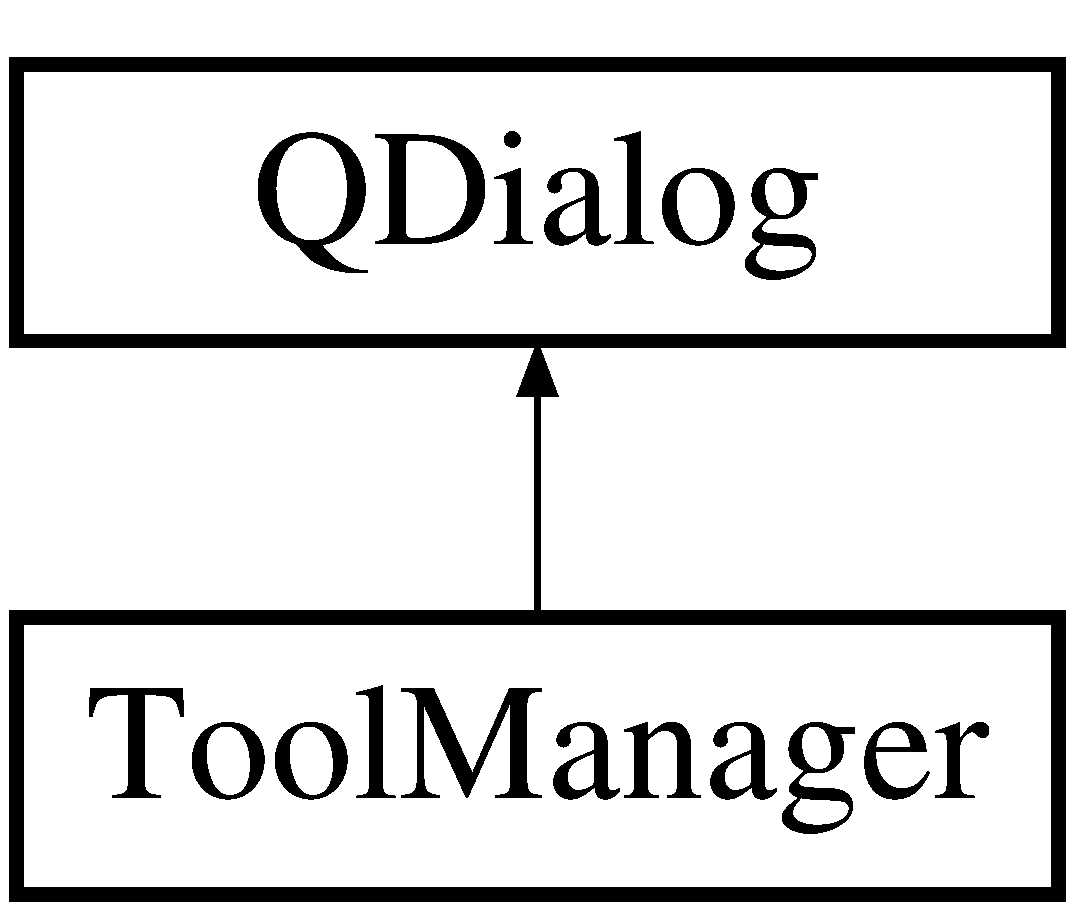
\includegraphics[height=2.000000cm]{classToolManager}
\end{center}
\end{figure}
\subsection*{Public Member Functions}
\begin{DoxyCompactItemize}
\item 
\hyperlink{classToolManager_ac69e222494ba128594c73d6545e50688}{Tool\-Manager} (Q\-Widget $\ast$parent, \hyperlink{classProperties}{Properties} $\ast$properties)
\begin{DoxyCompactList}\small\item\em Creates \hyperlink{classToolManager}{Tool\-Manager} object to give user an opportunity to choose tools for working with different view types. \end{DoxyCompactList}\item 
\hyperlink{classToolManager_a242d9f322f17b81946a921764ea6c5dd}{$\sim$\-Tool\-Manager} ()
\begin{DoxyCompactList}\small\item\em Destructs \hyperlink{classToolManager}{Tool\-Manager} obejct and clears up U\-I members. \end{DoxyCompactList}\end{DoxyCompactItemize}
\subsection*{Private Slots}
\begin{DoxyCompactItemize}
\item 
void \hyperlink{classToolManager_ad46d597d99731298489b34f4c25a6f00}{settings\-Changed} (Qt\-Property $\ast$, Q\-Variant)
\begin{DoxyCompactList}\small\item\em The slot is triggered once user changes tool settings. \end{DoxyCompactList}\item 
void \hyperlink{classToolManager_a2877a5eebdbf32bd984f58ba60087dfd}{on\-\_\-btn\-Ok\-\_\-clicked} ()
\begin{DoxyCompactList}\small\item\em Saves current tool settings into properties of \hyperlink{classMainWindow}{Main\-Window} object and closes the window. \end{DoxyCompactList}\item 
void \hyperlink{classToolManager_a5251e65adb28c3c8355ea2c16bfb2c2d}{on\-\_\-btn\-Cancel\-\_\-clicked} ()
\begin{DoxyCompactList}\small\item\em closes \hyperlink{classToolManager}{Tool\-Manager} window. \end{DoxyCompactList}\end{DoxyCompactItemize}
\subsection*{Private Member Functions}
\begin{DoxyCompactItemize}
\item 
void \hyperlink{classToolManager_a0ebfb9302faf76d53d4eafc48aad559a}{init} ()
\begin{DoxyCompactList}\small\item\em Initializes Qt\-Tree\-Property\-Browser and creates its properties. It's used to provide a list of tools that can be chosen by user to work with different view, documentation etc. \end{DoxyCompactList}\end{DoxyCompactItemize}
\subsection*{Private Attributes}
\begin{DoxyCompactItemize}
\item 
Ui\-::\-Tool\-Manager $\ast$ \hyperlink{classToolManager_a8cfa8377de1438e8eaa63d549cdeec44}{m\-\_\-ui}
\item 
\hyperlink{classMainWindow}{Main\-Window} $\ast$ \hyperlink{classToolManager_aaf5b5ff482e6fe661c5ba774c5fde50e}{m\-\_\-mw}
\item 
\hyperlink{classProperties}{Properties} $\ast$ \hyperlink{classToolManager_af7ce412063a8651c31441376504deda4}{m\-\_\-properties}
\item 
Qt\-Tree\-Property\-Browser $\ast$ \hyperlink{classToolManager_a6b9d5df12862696e13c561277f134e0d}{m\-\_\-pb\-Settings}
\item 
Qt\-Variant\-Property\-Manager $\ast$ \hyperlink{classToolManager_ac363f07b4d5b4d6b85f653d2590a730b}{m\-\_\-vm\-Settings}
\end{DoxyCompactItemize}


\subsection{Detailed Description}
The \hyperlink{classToolManager}{Tool\-Manager} class creates a dialog window to allow user controlling 3-\/d party tools executed by Lib\-Man. 



 

\subsection{Constructor \& Destructor Documentation}
\hypertarget{classToolManager_ac69e222494ba128594c73d6545e50688}{\index{Tool\-Manager@{Tool\-Manager}!Tool\-Manager@{Tool\-Manager}}
\index{Tool\-Manager@{Tool\-Manager}!ToolManager@{Tool\-Manager}}
\subsubsection[{Tool\-Manager}]{\setlength{\rightskip}{0pt plus 5cm}Tool\-Manager\-::\-Tool\-Manager (
\begin{DoxyParamCaption}
\item[{Q\-Widget $\ast$}]{parent, }
\item[{{\bf Properties} $\ast$}]{properties}
\end{DoxyParamCaption}
)\hspace{0.3cm}{\ttfamily [explicit]}}}\label{classToolManager_ac69e222494ba128594c73d6545e50688}


Creates \hyperlink{classToolManager}{Tool\-Manager} object to give user an opportunity to choose tools for working with different view types. 



 
\begin{DoxyParams}{Parameters}
{\em parent} & Parent widget, by default is N\-U\-L\-L. \\
\hline
{\em properties} & Container of Lib\-Man settings. \\
\hline
\end{DoxyParams}
\hypertarget{classToolManager_a242d9f322f17b81946a921764ea6c5dd}{\index{Tool\-Manager@{Tool\-Manager}!$\sim$\-Tool\-Manager@{$\sim$\-Tool\-Manager}}
\index{$\sim$\-Tool\-Manager@{$\sim$\-Tool\-Manager}!ToolManager@{Tool\-Manager}}
\subsubsection[{$\sim$\-Tool\-Manager}]{\setlength{\rightskip}{0pt plus 5cm}Tool\-Manager\-::$\sim$\-Tool\-Manager (
\begin{DoxyParamCaption}
{}
\end{DoxyParamCaption}
)}}\label{classToolManager_a242d9f322f17b81946a921764ea6c5dd}


Destructs \hyperlink{classToolManager}{Tool\-Manager} obejct and clears up U\-I members. 



 

\subsection{Member Function Documentation}
\hypertarget{classToolManager_a0ebfb9302faf76d53d4eafc48aad559a}{\index{Tool\-Manager@{Tool\-Manager}!init@{init}}
\index{init@{init}!ToolManager@{Tool\-Manager}}
\subsubsection[{init}]{\setlength{\rightskip}{0pt plus 5cm}void Tool\-Manager\-::init (
\begin{DoxyParamCaption}
{}
\end{DoxyParamCaption}
)\hspace{0.3cm}{\ttfamily [private]}}}\label{classToolManager_a0ebfb9302faf76d53d4eafc48aad559a}


Initializes Qt\-Tree\-Property\-Browser and creates its properties. It's used to provide a list of tools that can be chosen by user to work with different view, documentation etc. 



 \hypertarget{classToolManager_a5251e65adb28c3c8355ea2c16bfb2c2d}{\index{Tool\-Manager@{Tool\-Manager}!on\-\_\-btn\-Cancel\-\_\-clicked@{on\-\_\-btn\-Cancel\-\_\-clicked}}
\index{on\-\_\-btn\-Cancel\-\_\-clicked@{on\-\_\-btn\-Cancel\-\_\-clicked}!ToolManager@{Tool\-Manager}}
\subsubsection[{on\-\_\-btn\-Cancel\-\_\-clicked}]{\setlength{\rightskip}{0pt plus 5cm}void Tool\-Manager\-::on\-\_\-btn\-Cancel\-\_\-clicked (
\begin{DoxyParamCaption}
{}
\end{DoxyParamCaption}
)\hspace{0.3cm}{\ttfamily [private]}, {\ttfamily [slot]}}}\label{classToolManager_a5251e65adb28c3c8355ea2c16bfb2c2d}


closes \hyperlink{classToolManager}{Tool\-Manager} window. 



 \hypertarget{classToolManager_a2877a5eebdbf32bd984f58ba60087dfd}{\index{Tool\-Manager@{Tool\-Manager}!on\-\_\-btn\-Ok\-\_\-clicked@{on\-\_\-btn\-Ok\-\_\-clicked}}
\index{on\-\_\-btn\-Ok\-\_\-clicked@{on\-\_\-btn\-Ok\-\_\-clicked}!ToolManager@{Tool\-Manager}}
\subsubsection[{on\-\_\-btn\-Ok\-\_\-clicked}]{\setlength{\rightskip}{0pt plus 5cm}void Tool\-Manager\-::on\-\_\-btn\-Ok\-\_\-clicked (
\begin{DoxyParamCaption}
{}
\end{DoxyParamCaption}
)\hspace{0.3cm}{\ttfamily [private]}, {\ttfamily [slot]}}}\label{classToolManager_a2877a5eebdbf32bd984f58ba60087dfd}


Saves current tool settings into properties of \hyperlink{classMainWindow}{Main\-Window} object and closes the window. 



 \hypertarget{classToolManager_ad46d597d99731298489b34f4c25a6f00}{\index{Tool\-Manager@{Tool\-Manager}!settings\-Changed@{settings\-Changed}}
\index{settings\-Changed@{settings\-Changed}!ToolManager@{Tool\-Manager}}
\subsubsection[{settings\-Changed}]{\setlength{\rightskip}{0pt plus 5cm}void Tool\-Manager\-::settings\-Changed (
\begin{DoxyParamCaption}
\item[{Qt\-Property $\ast$}]{, }
\item[{Q\-Variant}]{}
\end{DoxyParamCaption}
)\hspace{0.3cm}{\ttfamily [private]}, {\ttfamily [slot]}}}\label{classToolManager_ad46d597d99731298489b34f4c25a6f00}


The slot is triggered once user changes tool settings. 



 

\subsection{Member Data Documentation}
\hypertarget{classToolManager_aaf5b5ff482e6fe661c5ba774c5fde50e}{\index{Tool\-Manager@{Tool\-Manager}!m\-\_\-mw@{m\-\_\-mw}}
\index{m\-\_\-mw@{m\-\_\-mw}!ToolManager@{Tool\-Manager}}
\subsubsection[{m\-\_\-mw}]{\setlength{\rightskip}{0pt plus 5cm}{\bf Main\-Window}$\ast$ Tool\-Manager\-::m\-\_\-mw\hspace{0.3cm}{\ttfamily [private]}}}\label{classToolManager_aaf5b5ff482e6fe661c5ba774c5fde50e}
A pointer to acess \hyperlink{classMainWindow}{Main\-Window} items as it's a friend class. \hypertarget{classToolManager_a6b9d5df12862696e13c561277f134e0d}{\index{Tool\-Manager@{Tool\-Manager}!m\-\_\-pb\-Settings@{m\-\_\-pb\-Settings}}
\index{m\-\_\-pb\-Settings@{m\-\_\-pb\-Settings}!ToolManager@{Tool\-Manager}}
\subsubsection[{m\-\_\-pb\-Settings}]{\setlength{\rightskip}{0pt plus 5cm}Qt\-Tree\-Property\-Browser$\ast$ Tool\-Manager\-::m\-\_\-pb\-Settings\hspace{0.3cm}{\ttfamily [private]}}}\label{classToolManager_a6b9d5df12862696e13c561277f134e0d}
A property browser framework enabling the user to edit a set of properties. \hypertarget{classToolManager_af7ce412063a8651c31441376504deda4}{\index{Tool\-Manager@{Tool\-Manager}!m\-\_\-properties@{m\-\_\-properties}}
\index{m\-\_\-properties@{m\-\_\-properties}!ToolManager@{Tool\-Manager}}
\subsubsection[{m\-\_\-properties}]{\setlength{\rightskip}{0pt plus 5cm}{\bf Properties}$\ast$ Tool\-Manager\-::m\-\_\-properties\hspace{0.3cm}{\ttfamily [private]}}}\label{classToolManager_af7ce412063a8651c31441376504deda4}
Container to store Lib\-Man settings. \hypertarget{classToolManager_a8cfa8377de1438e8eaa63d549cdeec44}{\index{Tool\-Manager@{Tool\-Manager}!m\-\_\-ui@{m\-\_\-ui}}
\index{m\-\_\-ui@{m\-\_\-ui}!ToolManager@{Tool\-Manager}}
\subsubsection[{m\-\_\-ui}]{\setlength{\rightskip}{0pt plus 5cm}Ui\-::\-Tool\-Manager$\ast$ Tool\-Manager\-::m\-\_\-ui\hspace{0.3cm}{\ttfamily [private]}}}\label{classToolManager_a8cfa8377de1438e8eaa63d549cdeec44}
A pointer to acess \hyperlink{classToolManager}{Tool\-Manager} graphic items. \hypertarget{classToolManager_ac363f07b4d5b4d6b85f653d2590a730b}{\index{Tool\-Manager@{Tool\-Manager}!m\-\_\-vm\-Settings@{m\-\_\-vm\-Settings}}
\index{m\-\_\-vm\-Settings@{m\-\_\-vm\-Settings}!ToolManager@{Tool\-Manager}}
\subsubsection[{m\-\_\-vm\-Settings}]{\setlength{\rightskip}{0pt plus 5cm}Qt\-Variant\-Property\-Manager$\ast$ Tool\-Manager\-::m\-\_\-vm\-Settings\hspace{0.3cm}{\ttfamily [private]}}}\label{classToolManager_ac363f07b4d5b4d6b85f653d2590a730b}
Each property type, the framework provides a property manager associated with editor factory. 

The documentation for this class was generated from the following files\-:\begin{DoxyCompactItemize}
\item 
toolmanager.\-h\item 
toolmanager.\-cpp\end{DoxyCompactItemize}

%--- End generated contents ---

% Index
\newpage
\phantomsection
\addcontentsline{toc}{part}{Index}
\printindex

\end{document}
